\documentclass[letterpaper]{article}
\usepackage[english]{babel}
\usepackage[utf8]{inputenc}
\usepackage{fullpage}
\usepackage{amsmath}
\usepackage{graphicx}
\usepackage[colorinlistoftodos]{todonotes}
\usepackage{hyperref}
\usepackage{amssymb}
\usepackage[T1]{fontenc}
\usepackage{mathtools}
\usepackage{amssymb}
\usepackage{mathrsfs}
\usepackage[noend]{algpseudocode}
\usepackage{fullpage}
\usepackage{times}
\usepackage{float}
\usepackage{fancyhdr,graphicx,amsmath,amssymb}
\usepackage[ruled,vlined]{algorithm2e}
\include{pythonlisting}
\usepackage{subcaption}
\setlength\parindent{0pt}
\usepackage[round]{natbib}
%\usepackage{titling}
%\setlength{\droptitle}{-7em}
\newcommand{\bz}{\mathbf{z}}
\newcommand{\bx}{\mathbf{x}}
\newcommand{\bmu}{\boldsymbol{\mu}}
\newcommand{\calN}{\mathcal{N}}
\newcommand{\bT}{\mathrm{T}}
\newcommand{\bc}{\mathbf{c}}
\newcommand{\bm}{\mathbf{m}}
\newcommand{\bs}{\mathbf{s}}
\newcommand{\bZ}{\mathbf{Z}}
\newcommand{\bpi}{\boldsymbol{\pi}}
\newcommand{\bX}{\mathbf{X}}
\newcommand{\bLambda}{\boldsymbol{\Lambda}}
\newcommand{\calW}{\mathcal{W}}
\newcommand{\balpha}{\boldsymbol{\alpha}}
\newcommand{\prodn}{\prod_{n=1}^N}
\newcommand{\prodk}{\prod_{k=1}^K}
\newcommand{\sumn}{\sum_{n=1}^N}
\newcommand{\sumk}{\sum_{k=1}^K}
\newcommand{\bW}{\mathbf{W}}
\newcommand{\bS}{\mathbf{S}}

%\usepackage{natbib}   % omit 'round' option if you prefer square brackets


\title{Variational Inference: A Review for Statisticians}
\author{Xiang Cui, Yutong Dai, Shuhui Guo}
\date{\today}
\begin{document}
\maketitle
\section{Introduction}
In the application generative probabilistic models, often introducing latent variables help govern the distribution of the data. In Bayesian statistics, one central task is to make inferences on the latent variables. Consider a joint density of latent variables $\bz=z_{1:m}$ and observations $\bx=x_{1:n}$,
\begin{alignat}{1}\label{eq:1}
p(\bz,\bx) = p(\bz)p(\bx | \bz)
\end{alignat}
where $p(\bz)$ is the prior density and $p(\bx|\bz)$ is the likelihood. In Bayesian inference, one is interested to find the posterior $p(\bz|\bx)$. However, in serious applications, this posterior is often hard to calculate. Markov chain Monte Carlo (MCMC) sampling is a traditional strategy, which can generate asymptotically exact samples from the target distribution \citep{robert2013monte}. However, it scales poorly to large datasets and complex models.

Variational inference (VI) has been proposed as an altervative method to approximate Bayesian inference which could scale to large dataset. Rather than use sampling in MCMC, variational inference uses the following optimization to do approximation. \begin{alignat}{2}\label{eq:2}
q^{\ast} (\bz) = \underset{q(\bz)\in \mathscr{Q}}{\operatorname{argmin}} \mathrm{KL} (q(\bz) || p(\bz|\bx))
\end{alignat}
where $\mathscr{Q}$ is a family of approximate densities, which is both flexible enough to capture the information in $p(\bz|\bx)$ and computationally tractable. And the Kullback-Leibler (KL) divergence measures the divergence of the approximate density $q(\bz)$ from the true posterior $p(\bz|\bx)$. Since VI solves an optimization problem, it is faster than MCMC. Therefore, variational inference is more appropriate for large-scale problems, such as document analysis, computational neuroscience, and computer vision. However, one has to point out that Variational inference might find local optimal and the approximated density often underestimated the variance of the true posterior density.

In this report, we will apply variational inference on the mixture of Gaussians and the numerical experiments can provide insights on its mechanism.

\section{Variational Inference}
\subsection{Approximate Inference}

Let $\bx=x_{1:n}$ be a set of observations and $\bz=z_{1:m}$ be a set of latent variables, with joint density $p(\bz,\bx)$. The inference problem is to compute the conditional density of the latent variables given the observation. The posterior $p(\bz|\bx)$ is calculated by
\begin{alignat}{3}\label{eq:3}
p(\bz|\bx) = \frac{p(\bz, \bx)}{p(\bx)}
\end{alignat}
%The denominator $p(\bx)$ is the marginal density of the observations, also called the evidence. It is calculated by
%\begin{alignat}{4}\label{eq:4}
%p(\bx) = \int p(\bz, \bx)d\bz
%\end{alignat}
%For many models, this evidence integral is unavailable in closed form or requires exponential time to compute, hence intractable.

The goal of variational inference is to find a $q(\bz)$ in a family of approximate densities $\mathscr{Q}$, satisfying the optimization
\begin{alignat}{5}\label{eq:5}
q^{\ast} (\bz) = \underset{q(\bz)\in \mathscr{Q}}{\operatorname{argmin}} \mathrm{KL} (q(\bz) || p(\bz|\bx))
\end{alignat}
where the $\mathrm{KL}$ divergence is calculated as
\begin{alignat}{6}\label{eq:6}
\mathrm{KL} (q(\bz) || p(\bz|\bx)) = \mathbb{E}[\mathrm{log}q(\bz)] - \mathbb{E}[\mathrm{log}p(\bz|\bx)]
\end{alignat}
where all expectations are taken with respect to $q(\bz)$. Expand the conditional,
\begin{alignat}{7}\label{eq:7}
\mathrm{KL} (q(\bz) || p(\bz|\bx)) = \mathbb{E}[\mathrm{log}q(\bz)] - \mathbb{E}[\mathrm{log}p(\bz, \bx)] + \mathrm{log}p(\bx)
\end{alignat}
Based on the above equation, the optimization problem is not computable because the evidence $\mathrm{log}p(\bx)$ is required to compute. Therefore, an alternative optimization objective is proposed as
\begin{alignat}{8}\label{eq:8}
\mathrm{ELBO}(q) = \mathbb{E}[\mathrm{log}p(\bz, \bx)] - \mathbb{E}[\mathrm{log}q(\bz)]
\end{alignat}
This function is called the evidence lower bound (ELBO). It lower-bounds the (log) evidence because
\begin{alignat}{9}\label{eq:9}
\mathrm{log}p(\bx) = \mathrm{KL} (q(\bz) || p(\bz|\bx)) + \mathrm{ELBO}(q)
\end{alignat}
The bound then follows from the fact that $\mathrm{KL} (\cdot) \geq 0$ \citep{kullback1951information}. Maximizing the ELBO equals to minimizing the KL divergence.

\subsection{The Mean-Field Variational Family}

We focus on the mean-field variational family to complete the specification of the optimization problem\eqref{eq:5}. The mean-field variational family refers to the family where the latent variables are mutually independent and each governed by a distinct factor in the variational density. A generic member of the mean-field variational family is
\begin{alignat}{10}\label{eq:10}
q(\bz) = \prod_{j=1}^m q_j(z_j)
\end{alignat}
Each latent variable $z_j$ is governed by its own variational factor, the density $q_j(z_j)$. In optimization, these variational factors are chosen to maximize the ELBO.

\subsection{Coordinate Ascent Mean-Field Variational Inference}

In solving this approximation optimization problem, coordinate ascent variational inference (CAVI) (Bishop, 2006) is one of the most commonly used algorithms. CAVI can iteratively optimize each factor of the mean-field variational density with the others fixed and find a local optimum for ELBO.

To derive the algorithm, we first need one result. Consider the $j$th latent variable $z_j$. The complete conditional of $z_j$ is its conditional density given all of the other latent variables in the model and observations, $p(z_j | \bz_{-j}, \bx)$. Fix the other variational factors $q_l (z_l), l\neq j$. The optimal $q_j(z_j)$ is
\begin{alignat}{11}\label{eq:11}
q^{\ast}_j (z_j) \propto \mathrm{exp}\{\mathbb{E}_{-j} [\mathrm{log}p(z_j | \bz_{-j}, \bx)]\}
\end{alignat}
The expectation in equation \eqref{eq:11} is with respect to the variational density over $\bz_{-j}$, that is, $\prod_{l\neq j} q_l (z_l)$. Equivalently, equation \eqref{eq:11} is proportional to the exponentiated log of the joint,

\begin{alignat}{12}\label{eq:12}
q^{\ast}_j (z_j) \propto \mathrm{exp}\{\mathbb{E}_{-j} [\mathrm{log}p(z_j , \bz_{-j}, \bx)]\}
\end{alignat}

Because all the latent variables are independent in the mean-field family, the expectations on the right hand side of \eqref{eq:12} do not involve the $j$th variational factor. Thus this is a valid coordinate update. This equation underlie the CAVI algorithm, presented in \textbf{Algorithm 1}. Through the iterations, the ELBO of equation \eqref{eq:8} will go uphill, eventually finding a local optimum.

\begin{algorithm}[H]
 \KwIn{A model $p(\bx,\bz)$, a data set $\bx$}
 \KwOut{A variational density $q(\bz) = \prod_{j=1}^m q_j(z_j)$}
 \textbf{Initialization} Variational factors $q_j(z_j)$ \\
 \While{the \text{ELBO} has not converged}{
     \textbf{for } $j \in \{1, \ldots, m\}$:  \\
     \textit{  Set } $q_j(z_j) \propto \text{exp}[\mathbb{E}_{-j}[\text{log }p(z_j|\textbf{z}_{-j},\textbf{x})]]$\\
     \textbf{end}\\
     Compute ELBO(q)
 }
 \textbf{end}\\
 \textbf{return} $q(z)$
  \caption{Coordinate ascent variational inference (CAVI)}
\end{algorithm}

Algorithm 1 CAVI is closely related to Gibbs sampling. The Gibbs sampler works in a way that iteratively samples the latent variables conditionally. And for CAVI, it uses the same complete conditional in equation \eqref{eq:11}.

\section{Bayesian Mixture of Gaussians}

\subsection{Unit-Variance Univariate Gaussian}

We will use multivariate Mixture of Gaussians with general model setup in our application. The paper\citep{blei2017variational} gives a variational inference method of Bayesian mixture of unit-variance univariate Gaussian. Hence, we only give a brief summary here.

For a Bayesian mixture of unit-variance univariate Gaussians, there are $K$ mixture components, corresponding to $K$ Gaussian distributions with means $\bmu = \{\mu_1,\dots, \mu_K \}$. The mean parameters are drawn independently from a common prior $p(\mu_k)$, which is assumed to be a Gaussian $\calN(0, \sigma^2)$, where the prior variance $\sigma^2$ is a parameter. To generate an observation $x_i$ from the model, a cluster assignment $c_i$ is first chosen. It indicates which latent cluster $x_i$ comes from and is drawn from a categorical distribution over $\{1,\dots,K \}$. $c_i$ is encoded as an indicator K-vector, all zeros except for a one in the position corresponding to $x_i$'s cluster. Then $x_i$ is drawn from the corresponding Gaussian $\calN(c^{\bT}_i \bmu, 1)$.

The full hierarchical model is
\begin{alignat}{13}
\mu_k &\sim \calN(0, \sigma^2) \quad k=1,\dots,K; \quad c_i \sim Categorical(1/K, \dots, 1/K) \quad i=1,\dots,n \\
x_i | c_i, \bmu &\sim \calN(c^{\bT}_i \bmu, 1) \quad i=1,\dots,n; \quad p(\bmu, \bc, \bx) = p(\bmu) \prod_{i=1}^n p(c_i)p(x_i | c_i, \bmu)
\end{alignat}
The latent variables are $\bz = \{ \bmu, \bc \}$, the $K$ class means and $n$ class assignments.

For estimation, the mean-field variational family contains approximate posterior densities of the form
\begin{alignat}{17}
q(\bmu, \bc) = \prod_{k=1}^K q(\mu_k;m_k, s_k^2) \prod_{i=1}^n q(c_i;\varphi_i) \label{eq:17}
\end{alignat}
In this equation, the factor $q(\mu_k;m_k, s_k^2)$ is a Gaussian distribution on the kth mixture component's mean parameter with mean $m_k$ and variance $s_k^2$. The factor $q(c_i;\varphi_i)$ is a distribution on the ith observation's mixture assignment with probabilities $\varphi_i$.

There are two types of variational parameters: categorical parameters $\varphi_i$ for approximating the posterior cluster assignment of the $i$th data point and the Gaussian parameters $m_k$ and $s_k^2$. 

%As a function of the variational parameters, the ELBO for the mixture of Gaussians are given by:

%\begin{alignat}{18}\label{eq:18}
%\begin{split}
%\mathrm{ELBO}(\bm, \bs^2, \mathrm{\varphi}) =& \sum_{k=1}^K \mathbb{E}[\mathrm{log}p(\mu_k);m_k, s_k^2] + \sum_{i=1}^n (\mathbb{E}[\mathrm{log}p(c_i);\varphi_i] + \mathbb{E}[\mathrm{log}p(x_i | c_i, \bmu);\varphi_i, \bm, \bs^2])\\
%&-\sum_{i=1}^n \mathbb{E}[\mathrm{log}q(c_i;\varphi_i)] - \sum_{k=1}^K \mathbb{E}[\mathrm{log}q(\mu_k);m_k, s_k^2]
%\end{split}
%\end{alignat}
%The CAVI algorithm updates each variational parameters in turn. 
%We then describe the update for each parameters.
%For the cluster assignment $c_i$, using equation $\eqref{eq:12}$, we could get:
%\begin{alignat}{19}\label{eq:19}
%q^{\ast} (c_i ;\varphi_i) \propto \mathrm{exp} \{\mathrm{log}p(c_i) + \mathbb{E}[\mathrm{log}p(x_i | c_i, \bmu); \bm, \bs^2] \}
%\end{alignat}
%The first term Equation $\eqref{eq:19}$ is $-logK$, the same for all possible values. For the second term, recall $p(x_i | c_i, \bmu) = \prod_{k=1}^K p(x_i | \mu_k)^{c_{ik}}$, we could get:
%\begin{alignat}{20}\label{eq:20}
%\mathbb{E}[\mathrm{log}p(x_i | c_i, \bmu)] &= \sum_k c_{ik} \mathbb{E}[\mathrm{log}p(x_i | \mu_k);m_k, s_k^2]
%\propto \sum_k c_{ik} (\mathbb{E}[\mu_k;m_k, s_k^2]x_i - \mathbb{E}[\mu_k^2;m_k, s_k^2]/2)
%\end{alignat}
%Therefore the update for the $i$th cluster assignment is:
%\begin{alignat}{21}\label{eq:21}
%\varphi_{ik} \propto \mathrm{exp} \{ \mathbb{E}[\mu_k;m_k, s_k^2]x_i - \mathbb{E}[\mu_k^2;m_k, s_k^2]/2 \}
%\end{alignat}

%Then we derive the variational density $q(\mu_k;m_k, s_k^2)$ of the $k$th mixture component. By $\eqref{eq:12}$,
%\begin{alignat}{22}\label{eq:22}
%q(\mu_k) \propto \mathrm{exp} \{ \mathrm{log}p(\mu_k) + \sum_{i=1}^n \mathbb{E}[\mathrm{log}p(x_i | c_i, \bmu);\varphi_i, \bm_{-k}, \bs_{-k}^2 ] \}
%\end{alignat}

%Recalling $\varphi_{ik}$ is the probability that the $i$th observation comes from the $k$th cluster, we can write $\varphi_{ik} = \mathbb{E}[c_{ik};\varphi_i]$. The unnormalized log of the coordinate-optimal $q(\mu_k)$ can be calculated as

%\begin{alignat}{23}
%\mathrm{log}q(\mu_k) &\propto \mathrm{log}p(\mu_k) + \sum_i \mathbb{E}[\mathrm{log}p(x_i | c_i, \bmu);\varphi_i, \bm_{-k}, \bs_{-k}^2] 
%\propto \mathrm{log}p(\mu_k) + \sum_i \mathbb{E}[c_{ik} \mathrm{log}p(x_i |\mu_k);\varphi_i] \\
%&\propto -\mu_k^2 /2\sigma^2 + \sum_i \mathbb{E}[c_{ik};\varphi_i] \mathrm{log}p(x_i |\mu_k) + \mathrm{const}
%\propto (\sum_i \varphi_{ik} x_i) \mu_k - (1/2 \sigma^2 + \sum_i \varphi_{ik} /2)\mu_k^2
%\end{alignat}
%This shows optimal variational density of $\mu_k$ is exponential family with sufficient statistics $\{\mu_k, \mu_k^2 \}$ and natural parameters $\{\sum_i \varphi_{ik} x_i, -\frac{1}{2}(1/\sigma^2 + \sum_i \varphi_{ik})\}$, expressed in terms of the variational mean and variance, the updates for $q(\mu_k)$ are
%\begin{alignat}{25}
%m_k = \frac{\sum_i \varphi_{ik} x_i}{1/\sigma^2 + \sum_i \varphi_{ik}}, \qquad s_k^2 = \frac{1}{1/\sigma^2 + \sum_i \varphi_{ik}}
%\end{alignat}
\textbf{Algorithm 2} presents the CAVI for the Bayesian mixture of Gaussians.

\begin{algorithm}[H]
 \KwIn{Data $x_{1:n}$, number of components $K$, prior variance of component means $\sigma^2$}
 \KwOut{Variational densities $q(\mu_k;m_k, s_k^2)$(Gaussian) and $q(c_i;\varphi_i)$(K-categorical)}
 \textbf{Initialization} Variational parameters $\bm=m_{1:K}, \bs^2=s_{1:K}^2$, and $\mathrm{\varphi}=\varphi_{1:n}$ \\
 \While{the ELBO has not converged}{
     \textbf{for } $j \in \{1,\dots, n\}$ \\ set $\varphi_{ik} \propto \mathrm{exp} \{ \mathbb{E}[\mu_k;m_k, s_k^2]x_i - \mathbb{E}[\mu_k^2;m_k, s_k^2]/2 \}$\\
     \textbf{end}\\
     \textbf{for } $k \in \{1,\dots, K\}$\\
     set $m_k \leftarrow \frac{\sum_i \varphi_{ik} x_i}{1/\sigma^2 + \sum_i \varphi_{ik}}$ and $s_k^2 \leftarrow \frac{1}{1/\sigma^2 + \sum_i \varphi_{ik}}$    \\
      \textbf{end}\\
     Compute $\mathrm{ELBO}(\bm, \bs^2, \mathrm{\varphi})$
 }
 \textbf{end}\\
 \textbf{return} $q(\bf{m, s^2, \varphi})$
  \caption{CAVI for Gaussian mixture model}
\end{algorithm}

Once the variational density is fitted, it can be used as the posterior. For example, we can obtain a posterior decomposition of the data. We assign points to their most likely mixture assignment $\hat{c}_i = \mathrm{argmax}_k \varphi_{ik}$ and estimate cluster means with their variational means $m_k$.

\subsection{Multivariate Gaussian Mixture Model}

For the model and CAVI algorithm presented in the paper \citep{blei2017variational}, it could only deal with unit-variance univariate Gaussian, but the dataset we deal with is multivariate mixture gaussians, we need a more general CAVI algorithm. Hence, we consider a CAVI algorithm for the multivariate mixture gaussian in the Book \citep{nasrabadi2007pattern}. 

The observed dataset is denoted by $\textbf{X} = \{x_1, \dots, x_n\}$. For each observation $x_n$, we have a corresponding latent variable $z_n$ comprising a 1-of-K binary vector with elements $z_{nk}$ for $k = 1,\ldots,K$. We denote the latent variables by $\textbf{Z} = \{z_1, \ldots, z_N\}$. The mixing coefficient is given by $\bpi = \{\pi_1,\ldots, \pi_K\}$,  where $p(z_{nk} = 1) = \pi_k$ and $\sum_{k = 1}^K\pi_k = 1$. Given the mixing coefficient, the conditional distribution of $\textbf{Z}$ could be written in the form;
\begin{alignat}{26}
p(\bZ | \bpi) = \prodn \prodk \pi_k^{z_{nk}}
\end{alignat}
And given the latent variables and component parameters, the conditional distribution of the observed data vectors could be given by:
\begin{alignat}{27}
p(\bX | \bZ, \bmu, \bLambda) = \prodn \prodk \calN (\bx_n | \bmu_k, \bLambda_k^{-1})^{z_{nk}}
\end{alignat}
where $\bmu_k$ and $\bLambda_k$ represent the mean vector and the precision matrix for the $k$-th mixture component. Then the joint distribution of all the random variables could be written as:
\begin{alignat}{28}
p(\bX, \bZ, \bpi, \bmu, \bLambda) = p(\bX | \bZ, \bmu, \bLambda) p(\bZ | \bpi) p(\bpi) p(\bmu | \bLambda) p(\bLambda)
\end{alignat}
where $\textbf{X} = \{x_1, \dots, x_n\}$ is the observed data. The prior over the mixing coefficient $\bpi$ is a Dirichlet distribution:
\begin{alignat}{29}\label{eq:29}
p(\bpi) = \mathrm{Dir}(\bpi | \balpha_0) = C(\balpha_0) \prodk \pi_k^{\alpha_0 -1}
\end{alignat} 
And for the mean and precision of each Gaussian component, we use the independent Gaussian-Wishart prior:
\begin{alignat}{30}
p(\bmu, \bLambda) &= p(\bmu | \bLambda)p(\bLambda) \label{eq:30}\\
& = \prodk \calN (\bmu_k | \mathbf{m}_0, (\beta_0 \bLambda_k)^{-1}) \calW (\bLambda_k | \mathbf{W}_0, v_0) \label{eq:31}
\end{alignat}
since this represents the conjugate prior distribution when both the mean and precision are unknown.

To estimate the posterior $p(\bZ, \bpi, \bmu, \bLambda |\bX) $, we consider a variational distribution which factorizes between the latent variables and the parameters, so that:
\begin{alignat}{32}
q(\bZ, \bpi, \bmu, \bLambda) = q(\bZ) q(\bpi, \bmu, \bLambda)
\end{alignat}
This is the only assumption that we need to make in order to obtain a tractable practical solution to the Bayesian Gaussian mixture model. The functional form of the factor $q(\bZ)$ and $q(\bpi, \bmu, \bLambda)$ will be determined automatically by optimizing the variation distribution, using the general result $\eqref{eq:12}$.

Then we derive the optimal sequential update equations for these factors: For the factor $q(\bZ)$, using the general result $\eqref{eq:12}$, the log of the optimized factor is given by:

\begin{alignat}{33}
\mathrm{ln} q^{\star}(\bZ) = \mathbb{E}_{\bpi, \bmu, \bLambda} [\mathrm{ln} p(\bX, \bZ, \bpi, \bmu, \bLambda)] +  \mathrm{const}
= \mathbb{E}_{\bpi} [\mathrm{ln} p(\bZ | \bpi)] + \mathbb{E}_{\bpi, \bLambda} [\mathrm{ln} p(\bX | \bZ, \bmu, \bLambda)] + \mathrm{const}
\end{alignat}
Substituting the two conditional distribution and absorbing the terms independent of $\bZ$, they get:
\begin{alignat}{34}\label{eq:34}
\mathrm{ln} q^{\star}(\bZ) = \sumn \sumk z_{nk} \mathrm{ln}\rho_{nk} + \mathrm{const}
\end{alignat}
where:
\begin{alignat}{35}
&\mathrm{ln}\rho_{nk} = \mathbb{E}[\mathrm{ln}\pi_k] + \frac{1}{2} \mathbb{E}[\mathrm{ln} |\bLambda_k|] - \frac{D}{2}\mathrm{ln} (2\pi) - \frac{1}{2}\mathbb{E}_{\bmu_k, \bLambda_k}[(\bx_n - \bmu_k)^{\bT} \bLambda_k (\bx_n - \bmu_k)] \label{eq:35} \\
&\mathbb{E}_{\bmu_k, \bLambda_k}[(\bx_n - \bmu_k)^{\bT} \bLambda_k (\bx_n - \bmu_k)] = D \beta_k^{-1} + v_k (\bx_n - \bm_k)^{\bT} \bW_k (\bx_n - \bm_k) \label{eq:36} \\
&\mathrm{ln}\widetilde{\Lambda}_k \equiv \mathbb{E}[\mathrm{ln}|\bLambda_k|] = \sum_{i=1}^D \psi (\frac{v_k +1-i}{2}) + D \mathrm{ln}2 + \mathrm{ln}|\bW_k|\label{eq:37} \\ 
&\mathrm{ln}\widetilde{\pi}_k \equiv \mathbb{E}[\mathrm{ln}\pi_k] = \psi(\alpha_k) - \psi(\hat{\alpha})\label{eq:38}
\end{alignat}

Taking the exponential of both sides of $\eqref{eq:34}$ and normalize this distribution, we could get the optimal solution for the factor $q(\bZ)$:
\begin{alignat}{39}\label{eq:39}
q^{\star}(\bZ) = \prodn \prodk r_{nk}^{z_{nk}} \quad \text{where} \quad r_{nk} = \frac{\rho_{nk}}{\sum_{j=1}^K \rho_{nj}}
\end{alignat}
At this point, it would be convenient for us to first define the following statsitcs:
\begin{alignat}{40}
N_k &= \sumn r_{nk}, \quad \bar{\bx}_k = \frac{1}{N_k} \sumn r_{nk} \bx_n \label{eq:40}\\
\bS_k &= \frac{1}{N_k} \sumn r_{nk} (\bx_n - \bar{\bx}_k)(\bx_n - \bar{\bx}_k)^{\bT} \label{eq:41}
\end{alignat}
Then we could consider the factor $q(\bpi, \bf{u}, \bLambda)$, again using the general result $\eqref{eq:12}$ we have:
\begin{alignat}{42}\label{eq:42}
\mathrm{ln} q^{\star}(\bpi, \bmu, \bLambda) = \mathrm{ln} p(\bpi) + \sumk \mathrm{ln} p(\bmu_k, \bLambda_k) + \mathbb{E}_{\bZ} [\mathrm{ln} p(\bZ | \bpi)] + \sumk \sumn \mathbb{E}[z_{nk}] \mathrm{ln} \calN (\bx_n | \bmu_k, \bLambda_k^{-1}) + \mathrm{const}
\end{alignat}
where we could see that the right-hand side of this expression could decompose into a sum of terms involving $\pi$ only and another sum of terms involving $\bmu$ and $\bLambda$, which imply the variational posterior $q(\bpi, \bmu, \bLambda)$ could factorize to give $q(\bpi)q(\bf{\mu},\bLambda)$, hence we could get:
\begin{alignat}{43}\label{eq:43}
q(\bpi, \bmu, \bLambda) = q(\bpi) \prodk q(\bmu_k, \bLambda_k)
\end{alignat}
Identifying the terms on the right hand of \eqref{eq:42}, we could get:
\begin{alignat}{44}\label{eq:44}
\mathrm{ln} q^{\star}(\bpi) = (\alpha_0 - 1) \sumk \mathrm{ln} \pi_k + \sumk \sumn r_{nk} \mathrm{ln} \pi_k + \mathrm{const}
\end{alignat}
Take the exponential on both sides, we could identify:
\begin{alignat}{45}\label{eq:45}
q^{\star}(\bpi) = \mathrm{Dir}(\bpi | \balpha) \quad \alpha_k = \alpha_0 + N_k
\end{alignat}
Also by identifying the terms on the right hand of \eqref{eq:42}, we could get:
\begin{alignat}{46}\label{eq:46}
q^{\star}(\bmu_k, \bLambda_k) = \calN(\bmu_k | \bm_k, (\beta_k \bLambda_k)^{-1}) \calW(\bLambda_k | \bW_k, v_k)
\end{alignat}
where 
\begin{alignat}{47}
\beta_k &= \beta_0 + N_k, \quad \bm_k = \frac{1}{\beta_k} (\beta_0 \bm_0 + N_k \bar{\bx}_k) \label{eq:47}\\
\bW_k^{-1} &= \bW_0^{-1} + N_k \bS_k + \frac{\beta_0 N_k}{\beta_0 + N_k} (\bar{\bx}_k - \bm_0)(\bar{\bx}_k - \bm_0)^{\bT}, \quad v_k = v_0 + N_k \label{eq:48}
\end{alignat}
In order to test for convergence, we also use the ELBO in equation \eqref{eq:7}.

In general, the optimization of the variational distribution involves two stages: the first stage is using the current model parameters to evaluate the moments in \eqref{eq:36}, \eqref{eq:37}, \eqref{eq:38}; the second stage is to keep these moment as constant and recompute the different model parameters through \eqref{eq:35}, \eqref{eq:39}, \eqref{eq:45}, \eqref{eq:46},\eqref{eq:47},\eqref{eq:48}. Cycling the above two stages until the ELBO value converges could give us the optimal solution for the variational distribution.

\begin{algorithm}[H]
 \KwIn{Data $X = x_{1:N}$, number of components $K$, prior for $\bpi$ in \eqref{eq:29}, independent Gaussian-Wishart prior for $\bmu,\bLambda$ in  \eqref{eq:31}} 
 \KwOut{Variational densities for latent variables $q(\bZ)$ and for parameter $q(\bpi)$ and  $q(\bmu_k, \bLambda_k)$}
 \textbf{Initialization} Variational parameters in $q(\bZ)$, $q(\bpi)$ and  $q(\bmu_k, \bLambda_k)$\\
 \While{the ELBO has not converged}{
    Evaluate the moment $\mathbb{E}_{\bmu_k, \bLambda_k}[(\bx_n - \bmu_k)^{\bT} \bLambda_k (\bx_n - \bmu_k)] , \mathbb{E}[\mathrm{ln}|\bLambda_k|]$ and $\mathbb{E}[\mathrm{ln}\pi_k]$ as in \eqref{eq:36}, \eqref{eq:37}, \eqref{eq:38}\\
Update the optimal density for $q^*(Z)$ as in \eqref{eq:35}, \eqref{eq:39}\\
Update the statistics in \eqref{eq:40}, \eqref{eq:41}\\
Update the optimal density for $q^*(\bpi)$ as in \eqref{eq:45}\\
Update the optimal density for $q^*(\bmu_k,\bLambda_k)$ as in \eqref{eq:46},\eqref{eq:47},\eqref{eq:48}\\
Compute $\mathrm{ELBO}$ as in \eqref{eq:8}
 }
 \textbf{end}\\
 \textbf{return} $q(\bZ)$, $q(\bpi)$, $q(\bmu, \bLambda)$
  \caption{CAVI for Multivariate Gaussian mixture model}
  \label{alg:3}
\end{algorithm}
\section{Experiment}
\subsection{Simulation}
\begin{figure}[H]
  \centering
  \begin{subfigure}[b]{0.25\linewidth}
    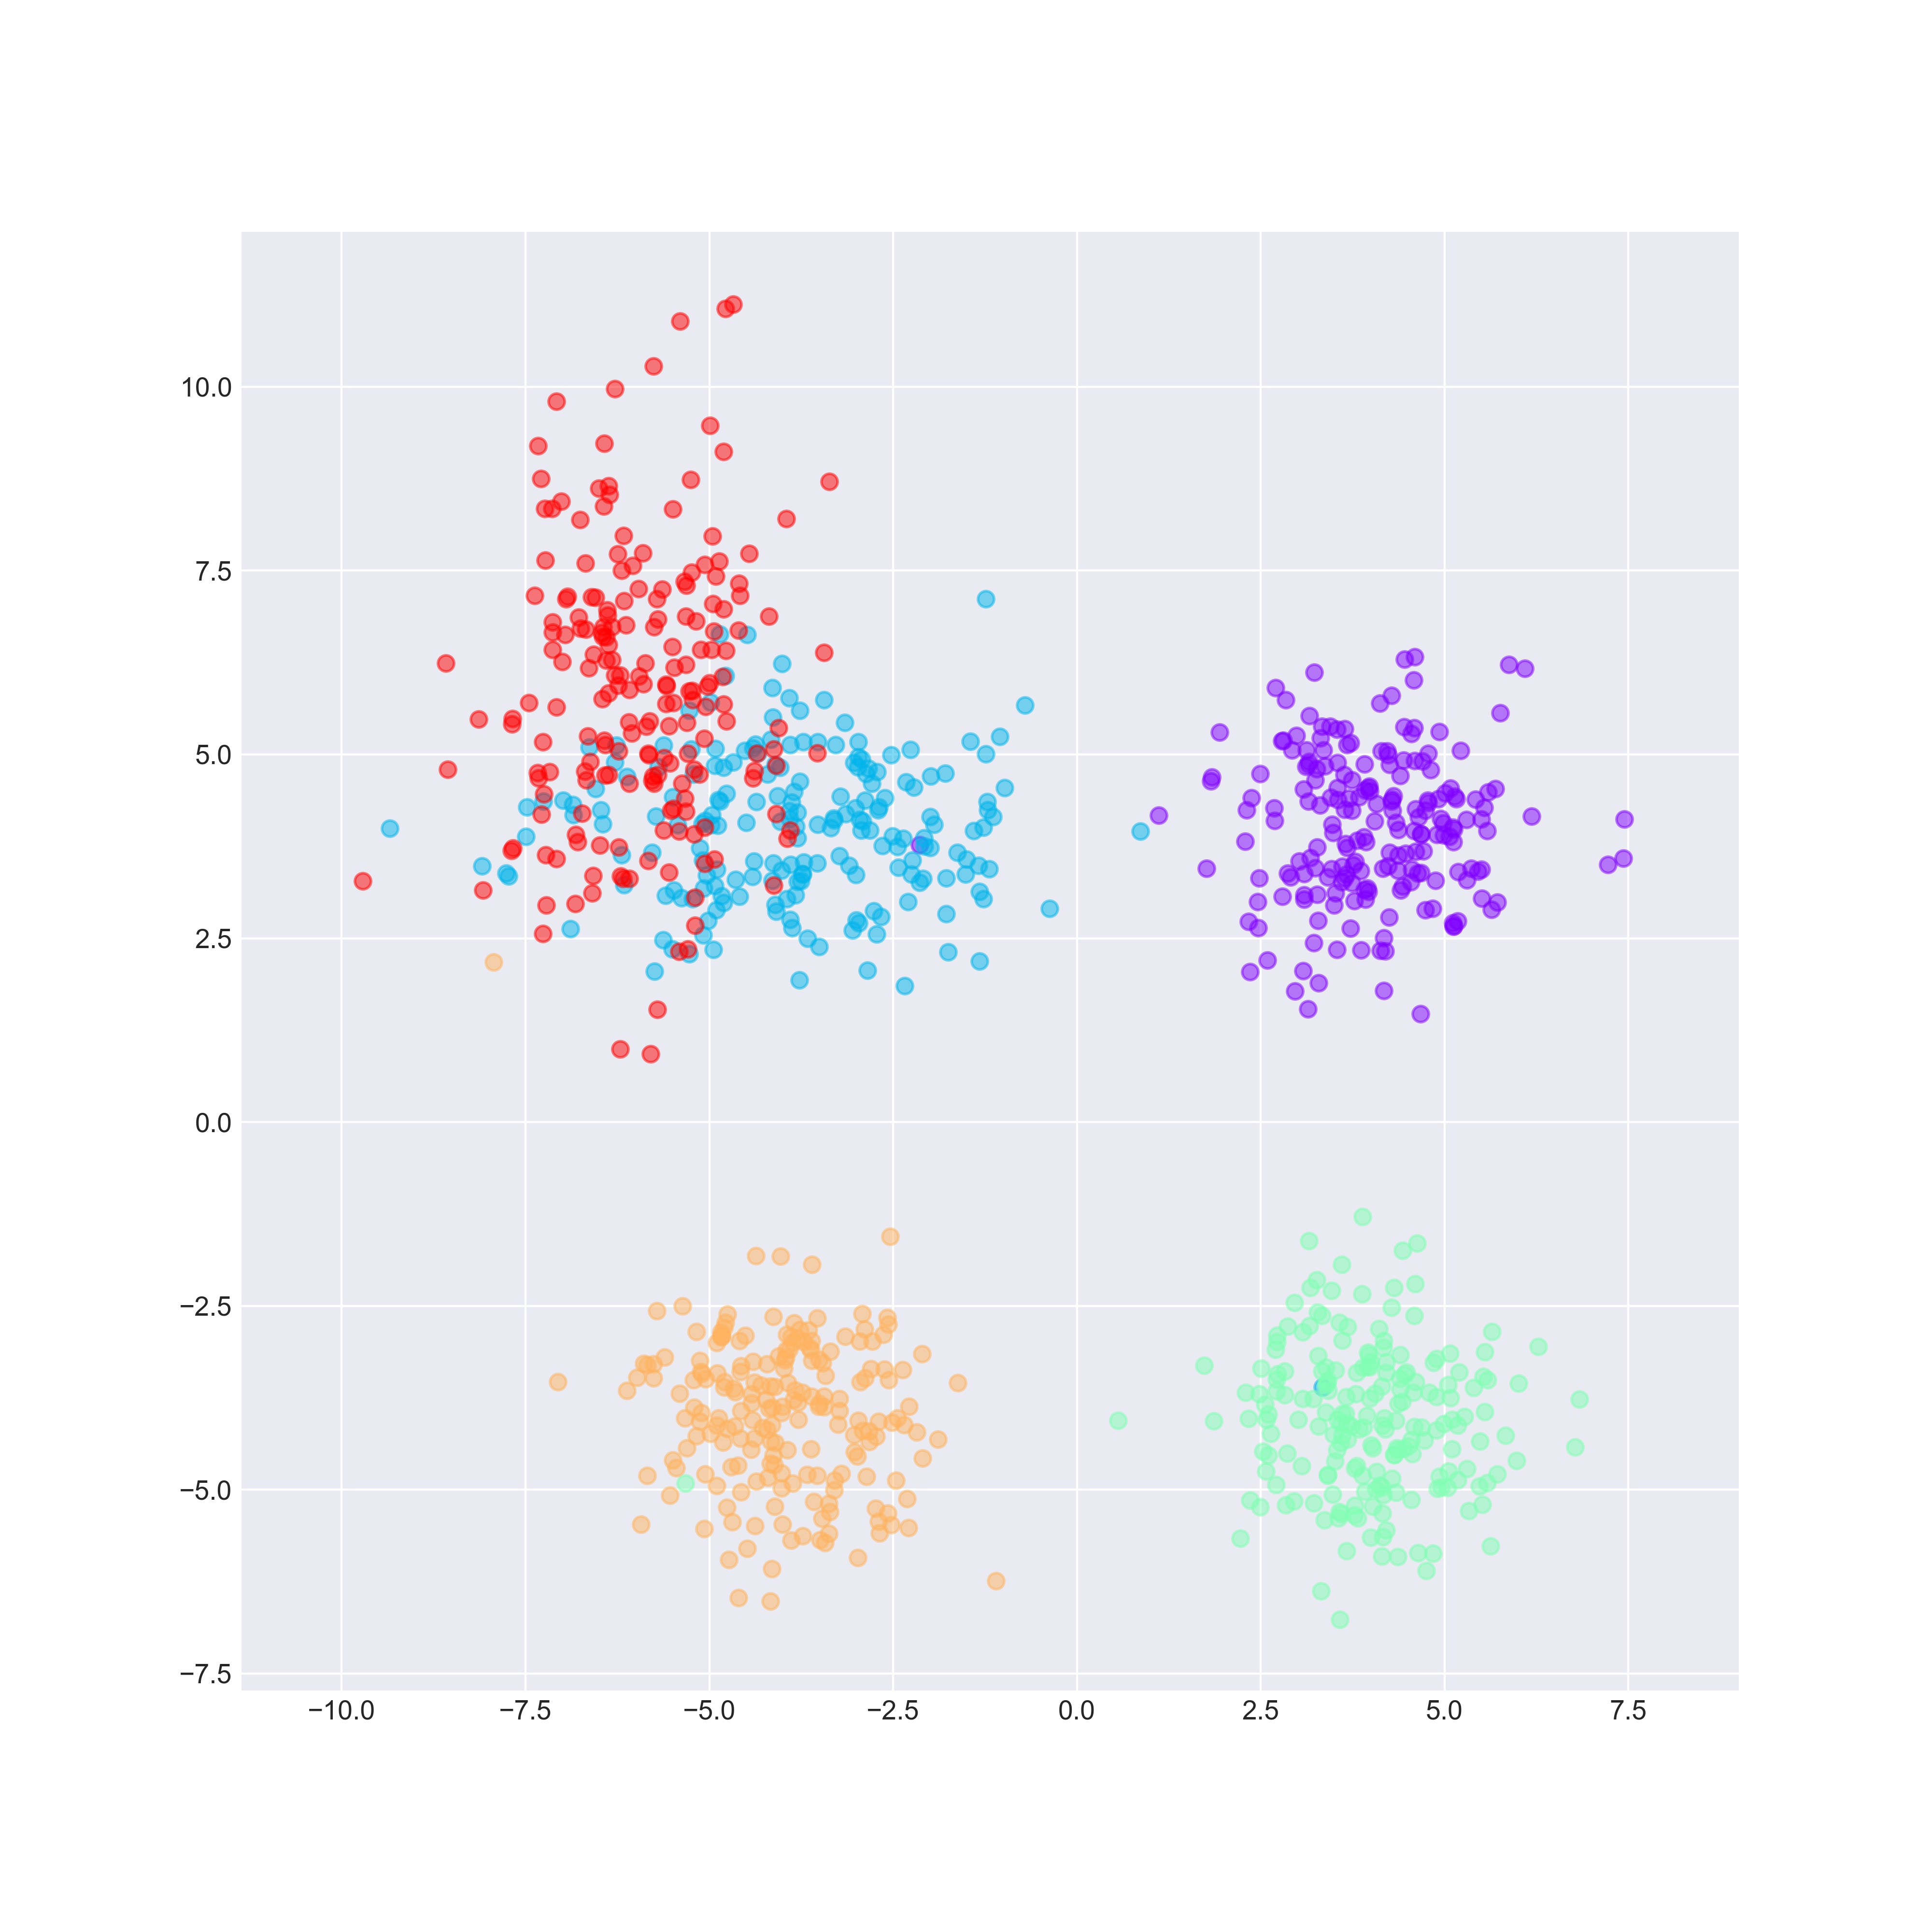
\includegraphics[width=\linewidth]{outputs/report_figs/simulation_original.jpeg}
     \caption{Simulated data}
  \end{subfigure}
  \begin{subfigure}[b]{0.25\linewidth}
    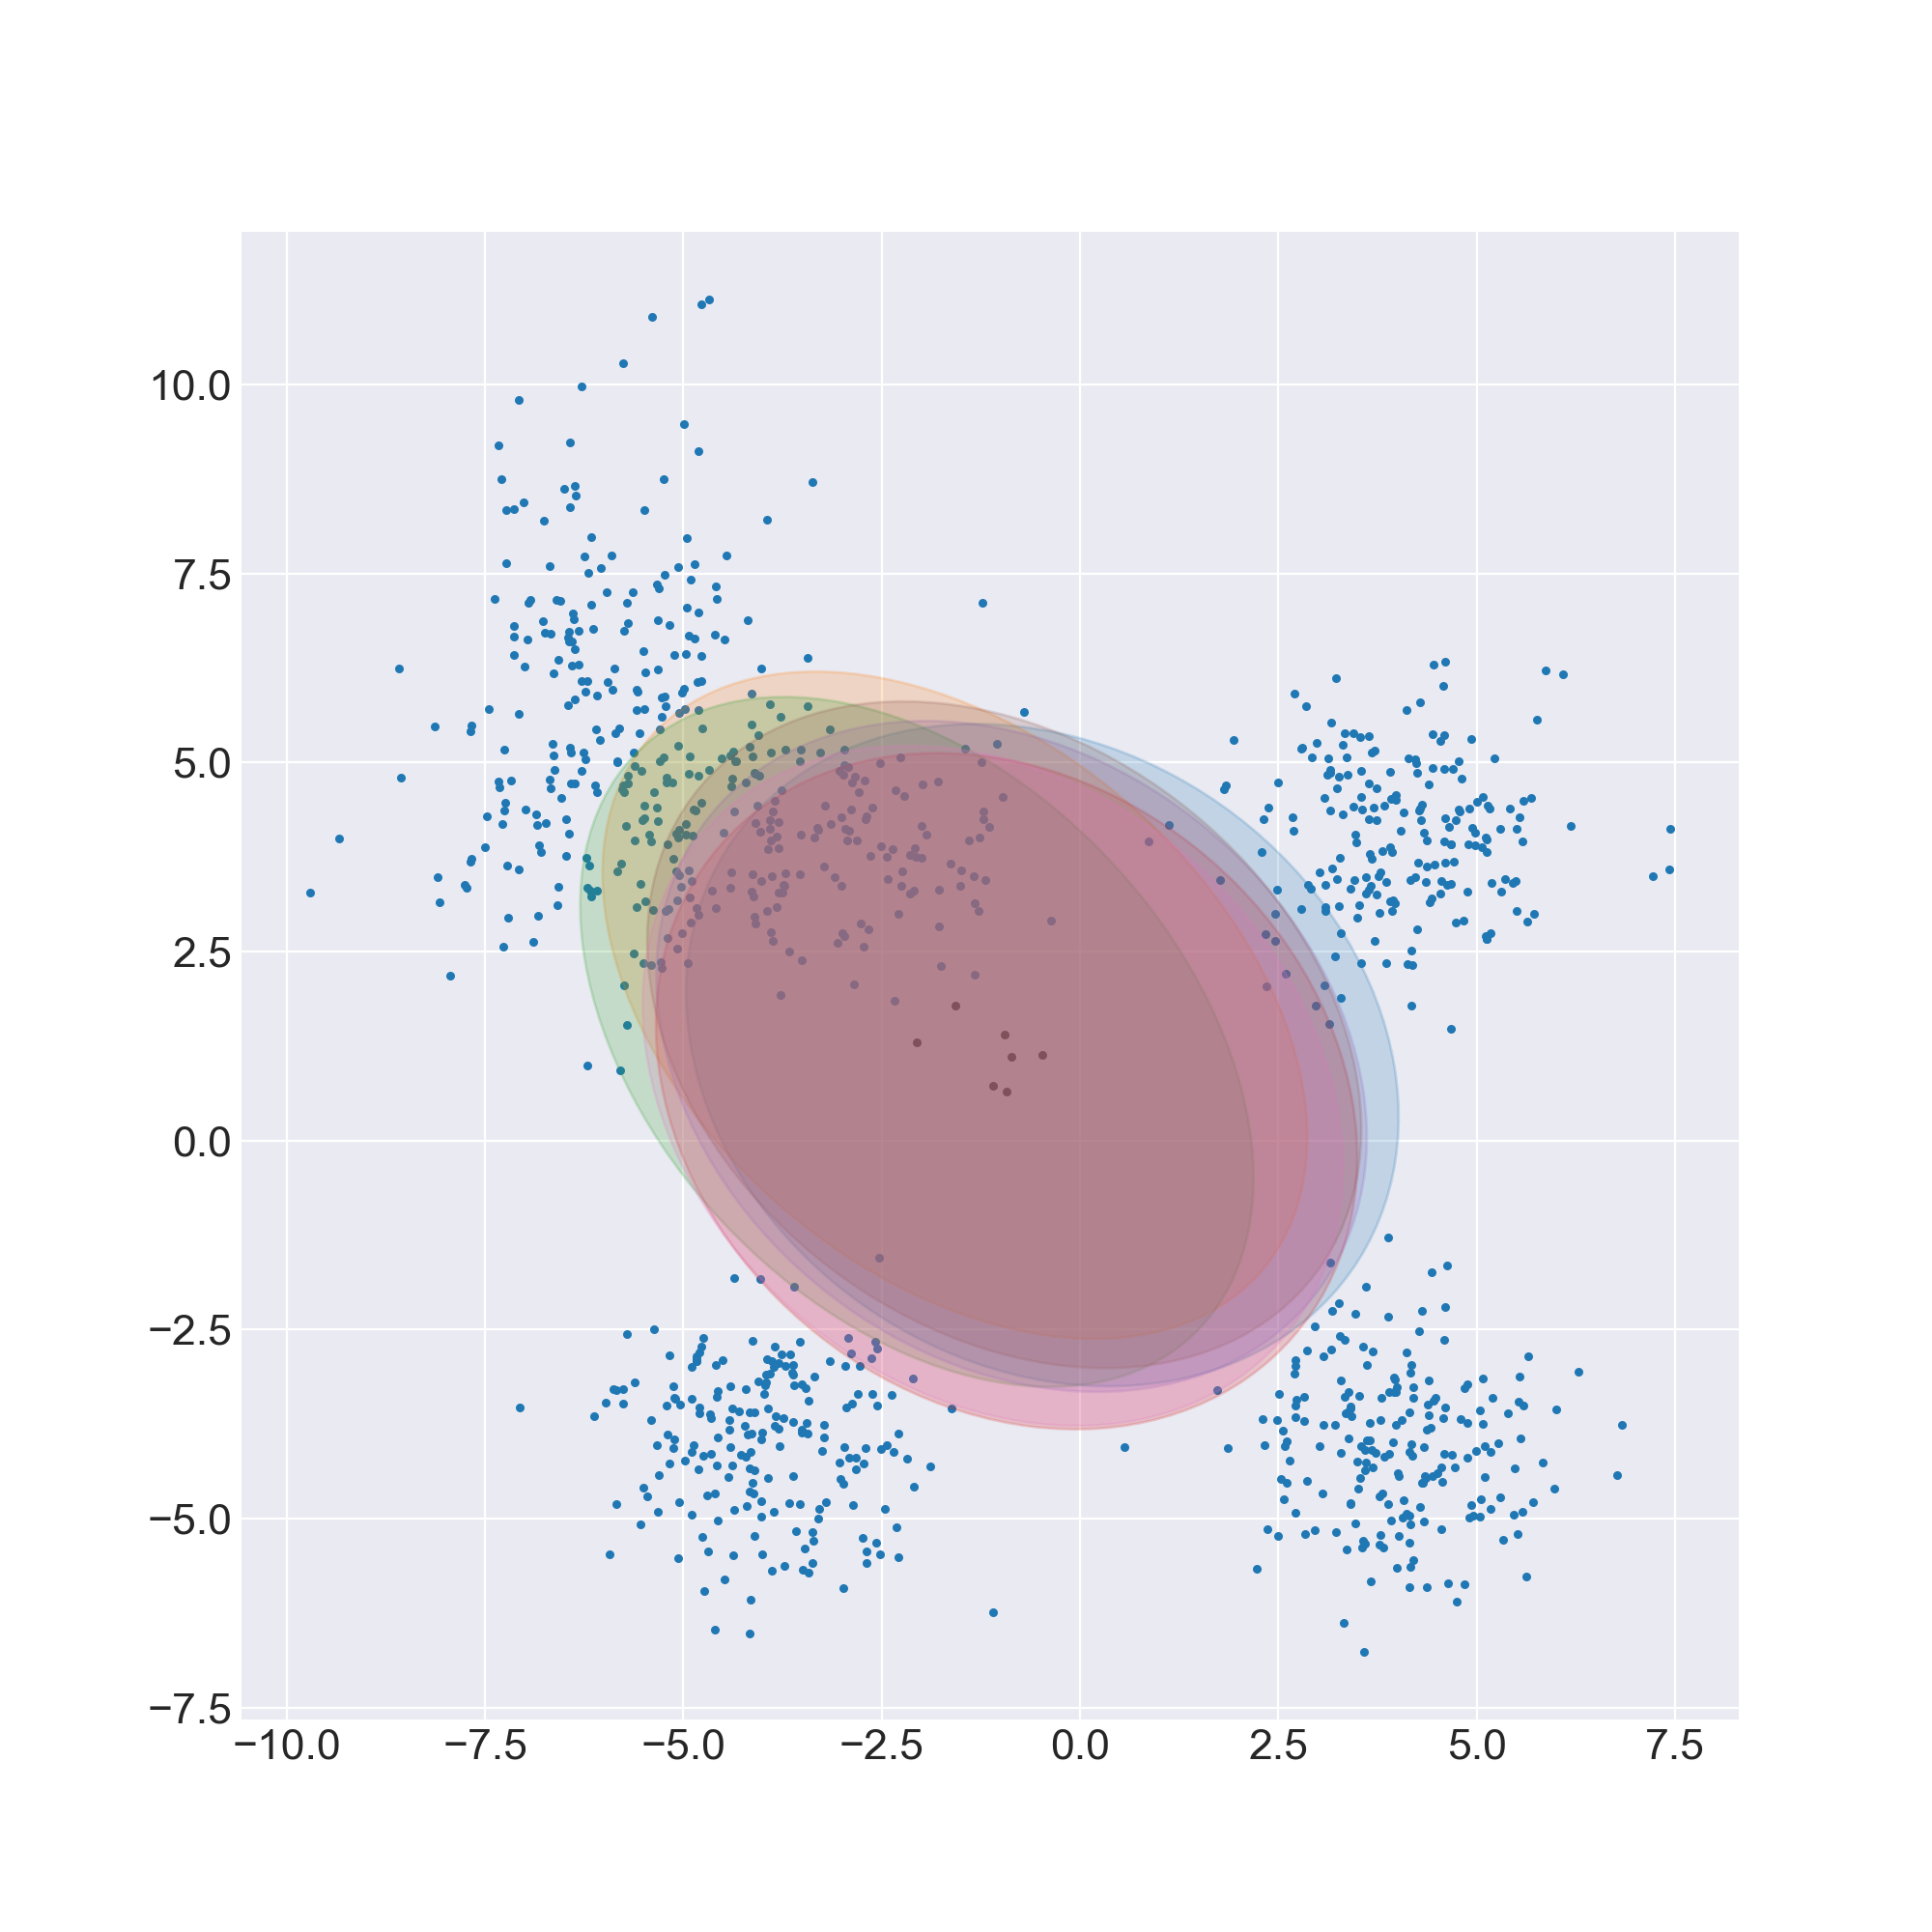
\includegraphics[width=\linewidth]{outputs/simulation/iter_10.png}
    \caption{Iteration 10}
  \end{subfigure}
 \begin{subfigure}[b]{0.25\linewidth}
   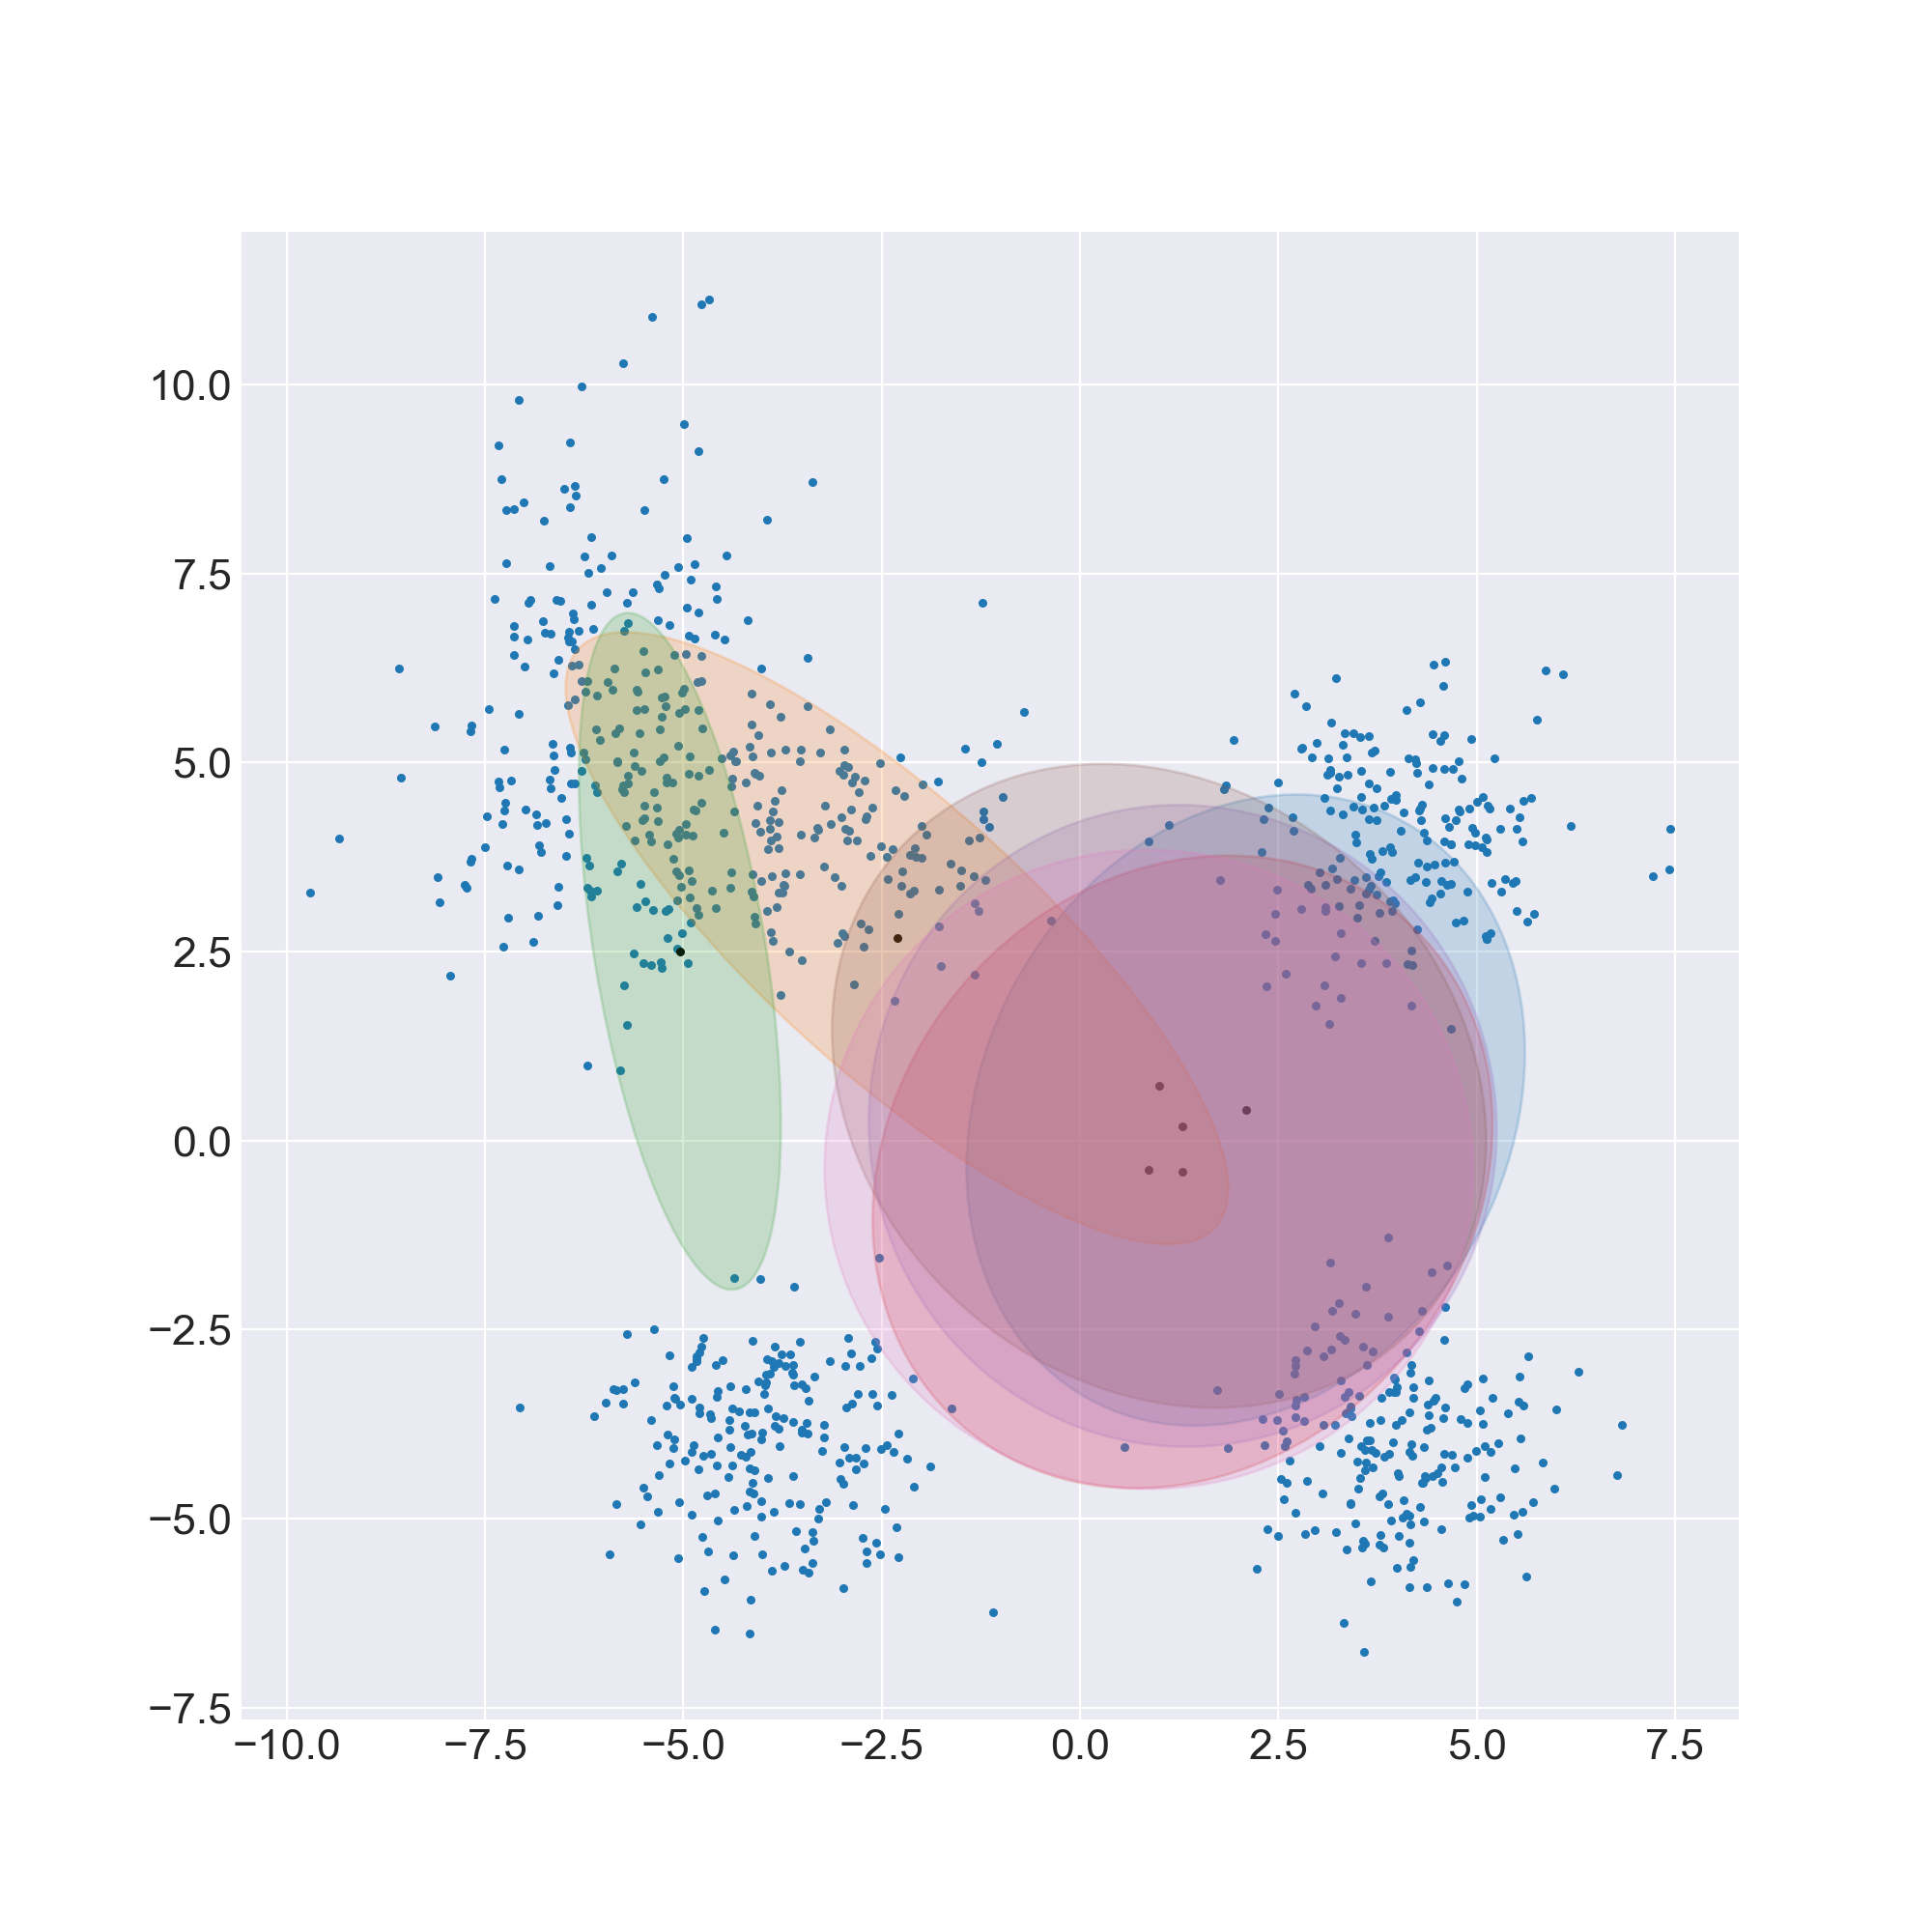
\includegraphics[width=\linewidth]{outputs/simulation/iter_20.png}
    \caption{Iteration 20}
  \end{subfigure}
  \begin{subfigure}[b]{0.25\linewidth}
    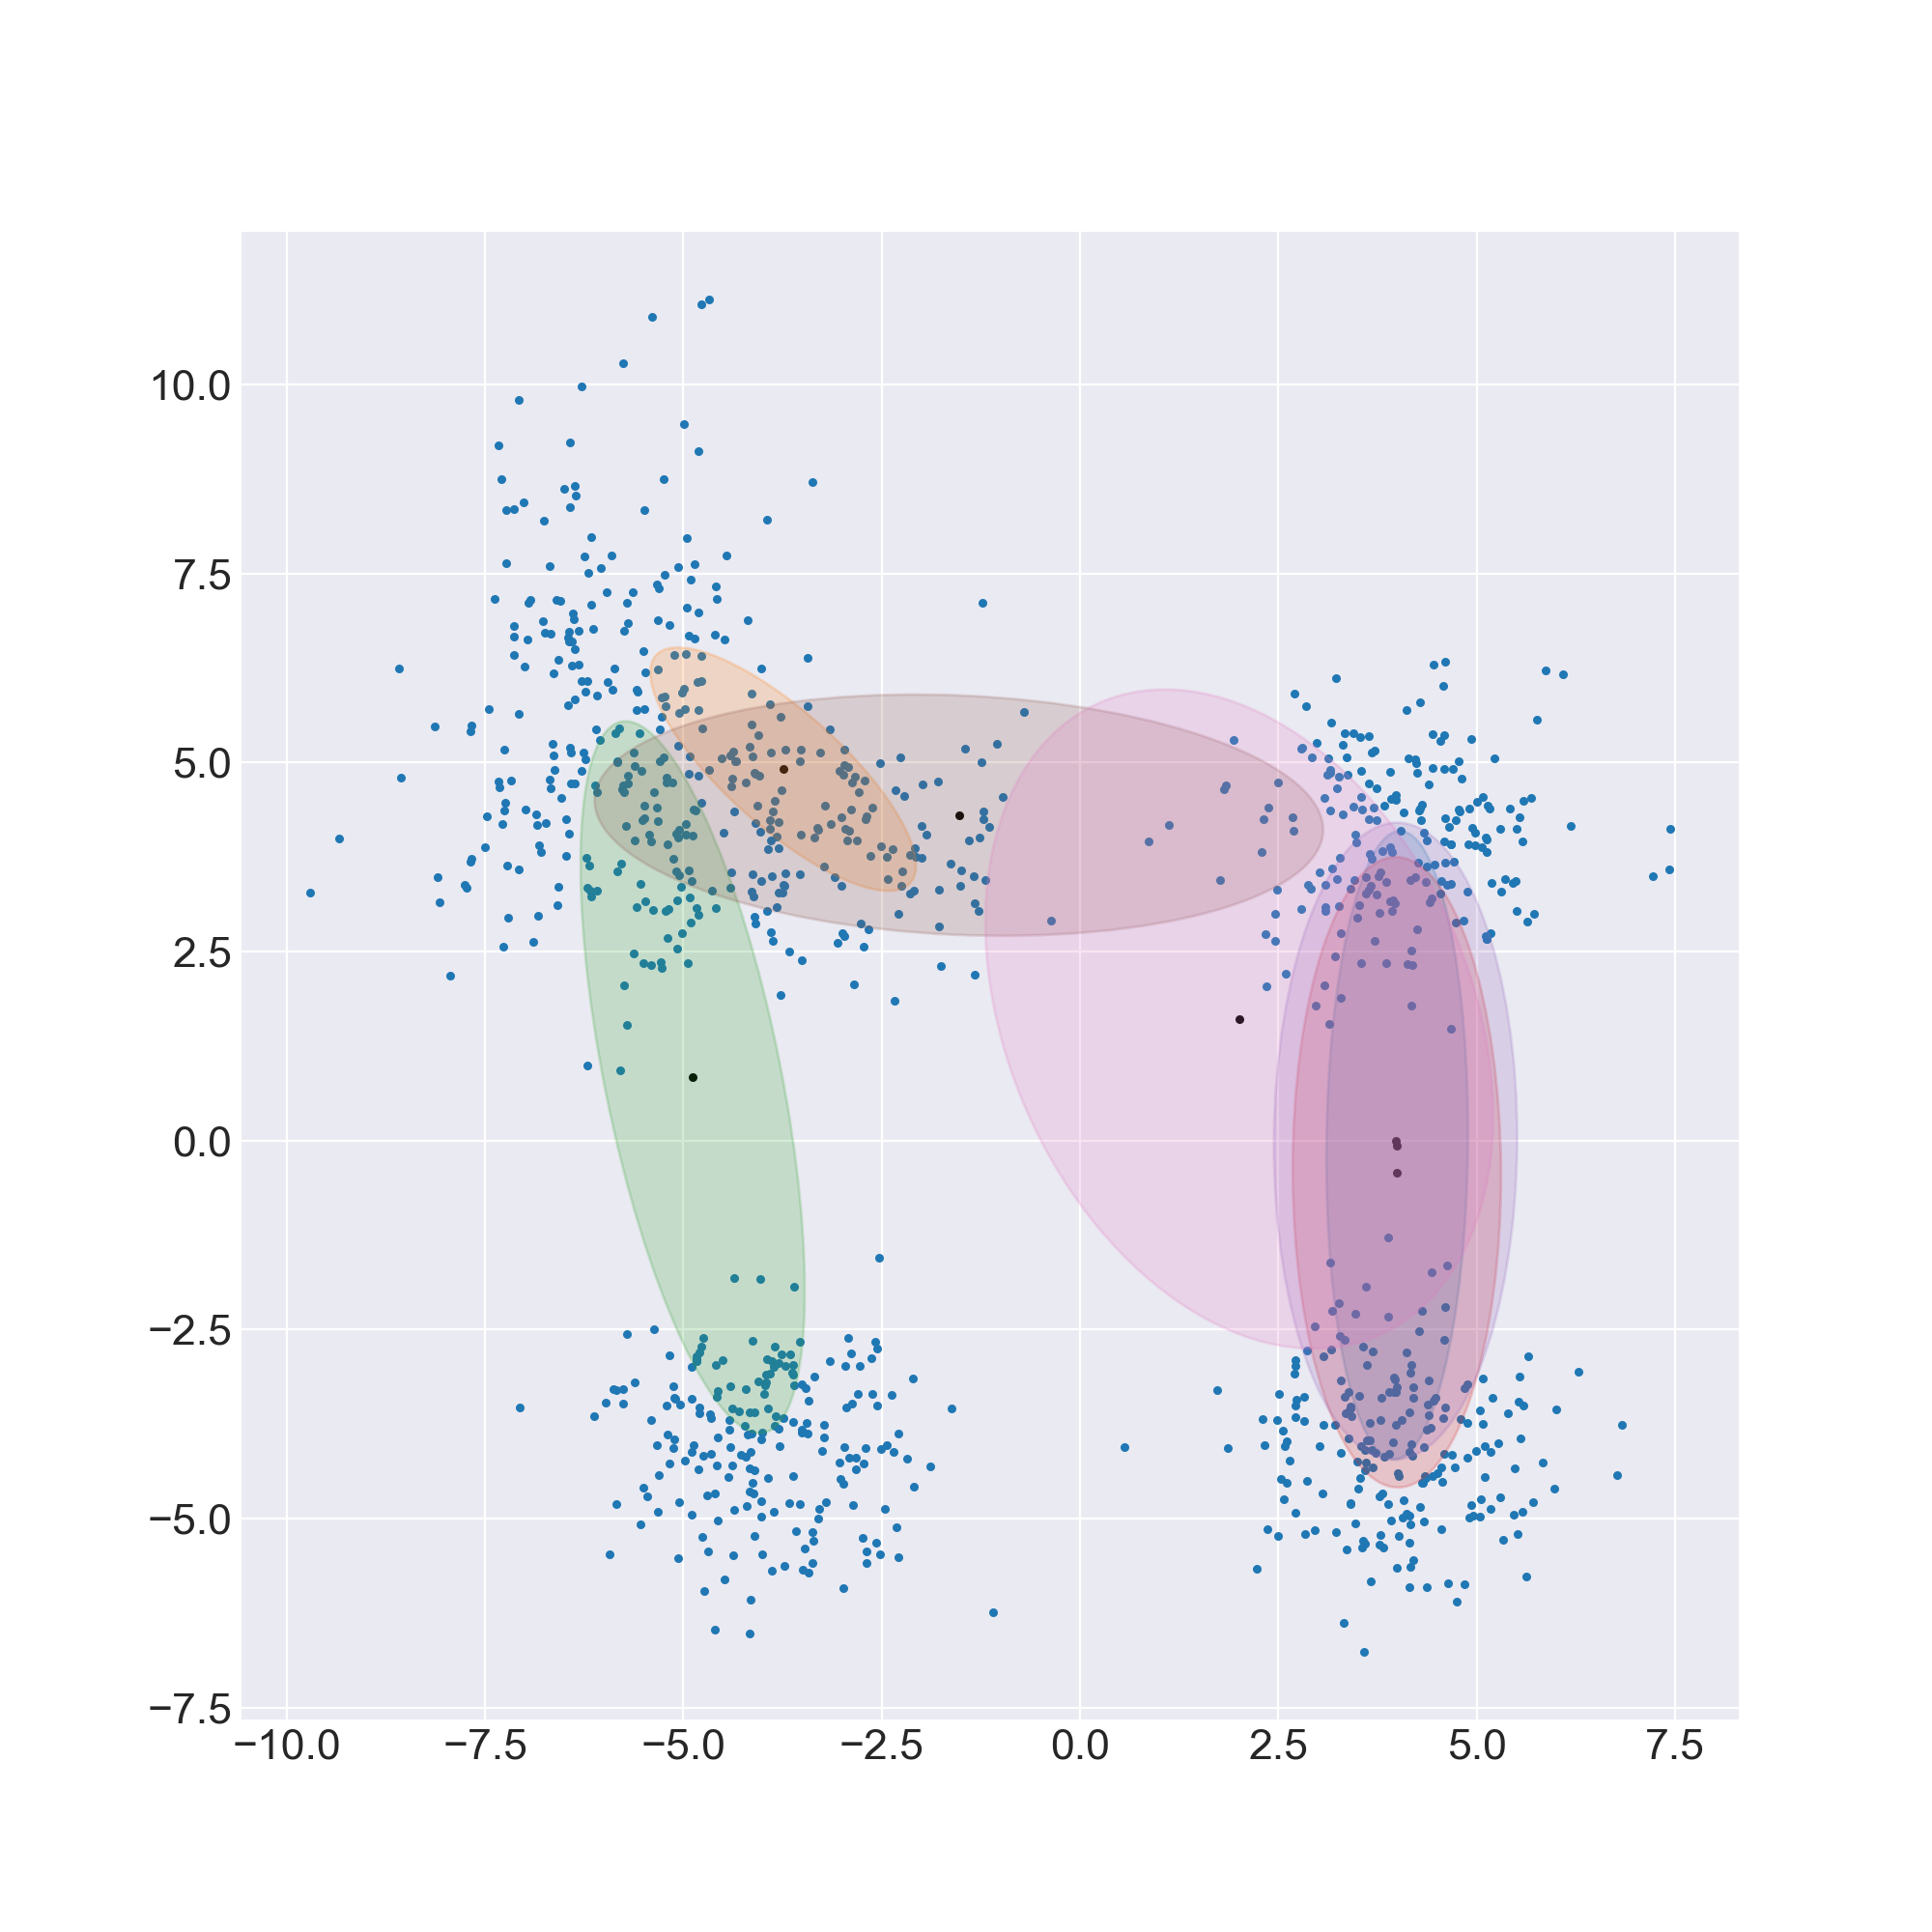
\includegraphics[width=\linewidth]{outputs/simulation/iter_30.png}
     \caption{Iteration 30}
  \end{subfigure}
  \begin{subfigure}[b]{0.25\linewidth}
    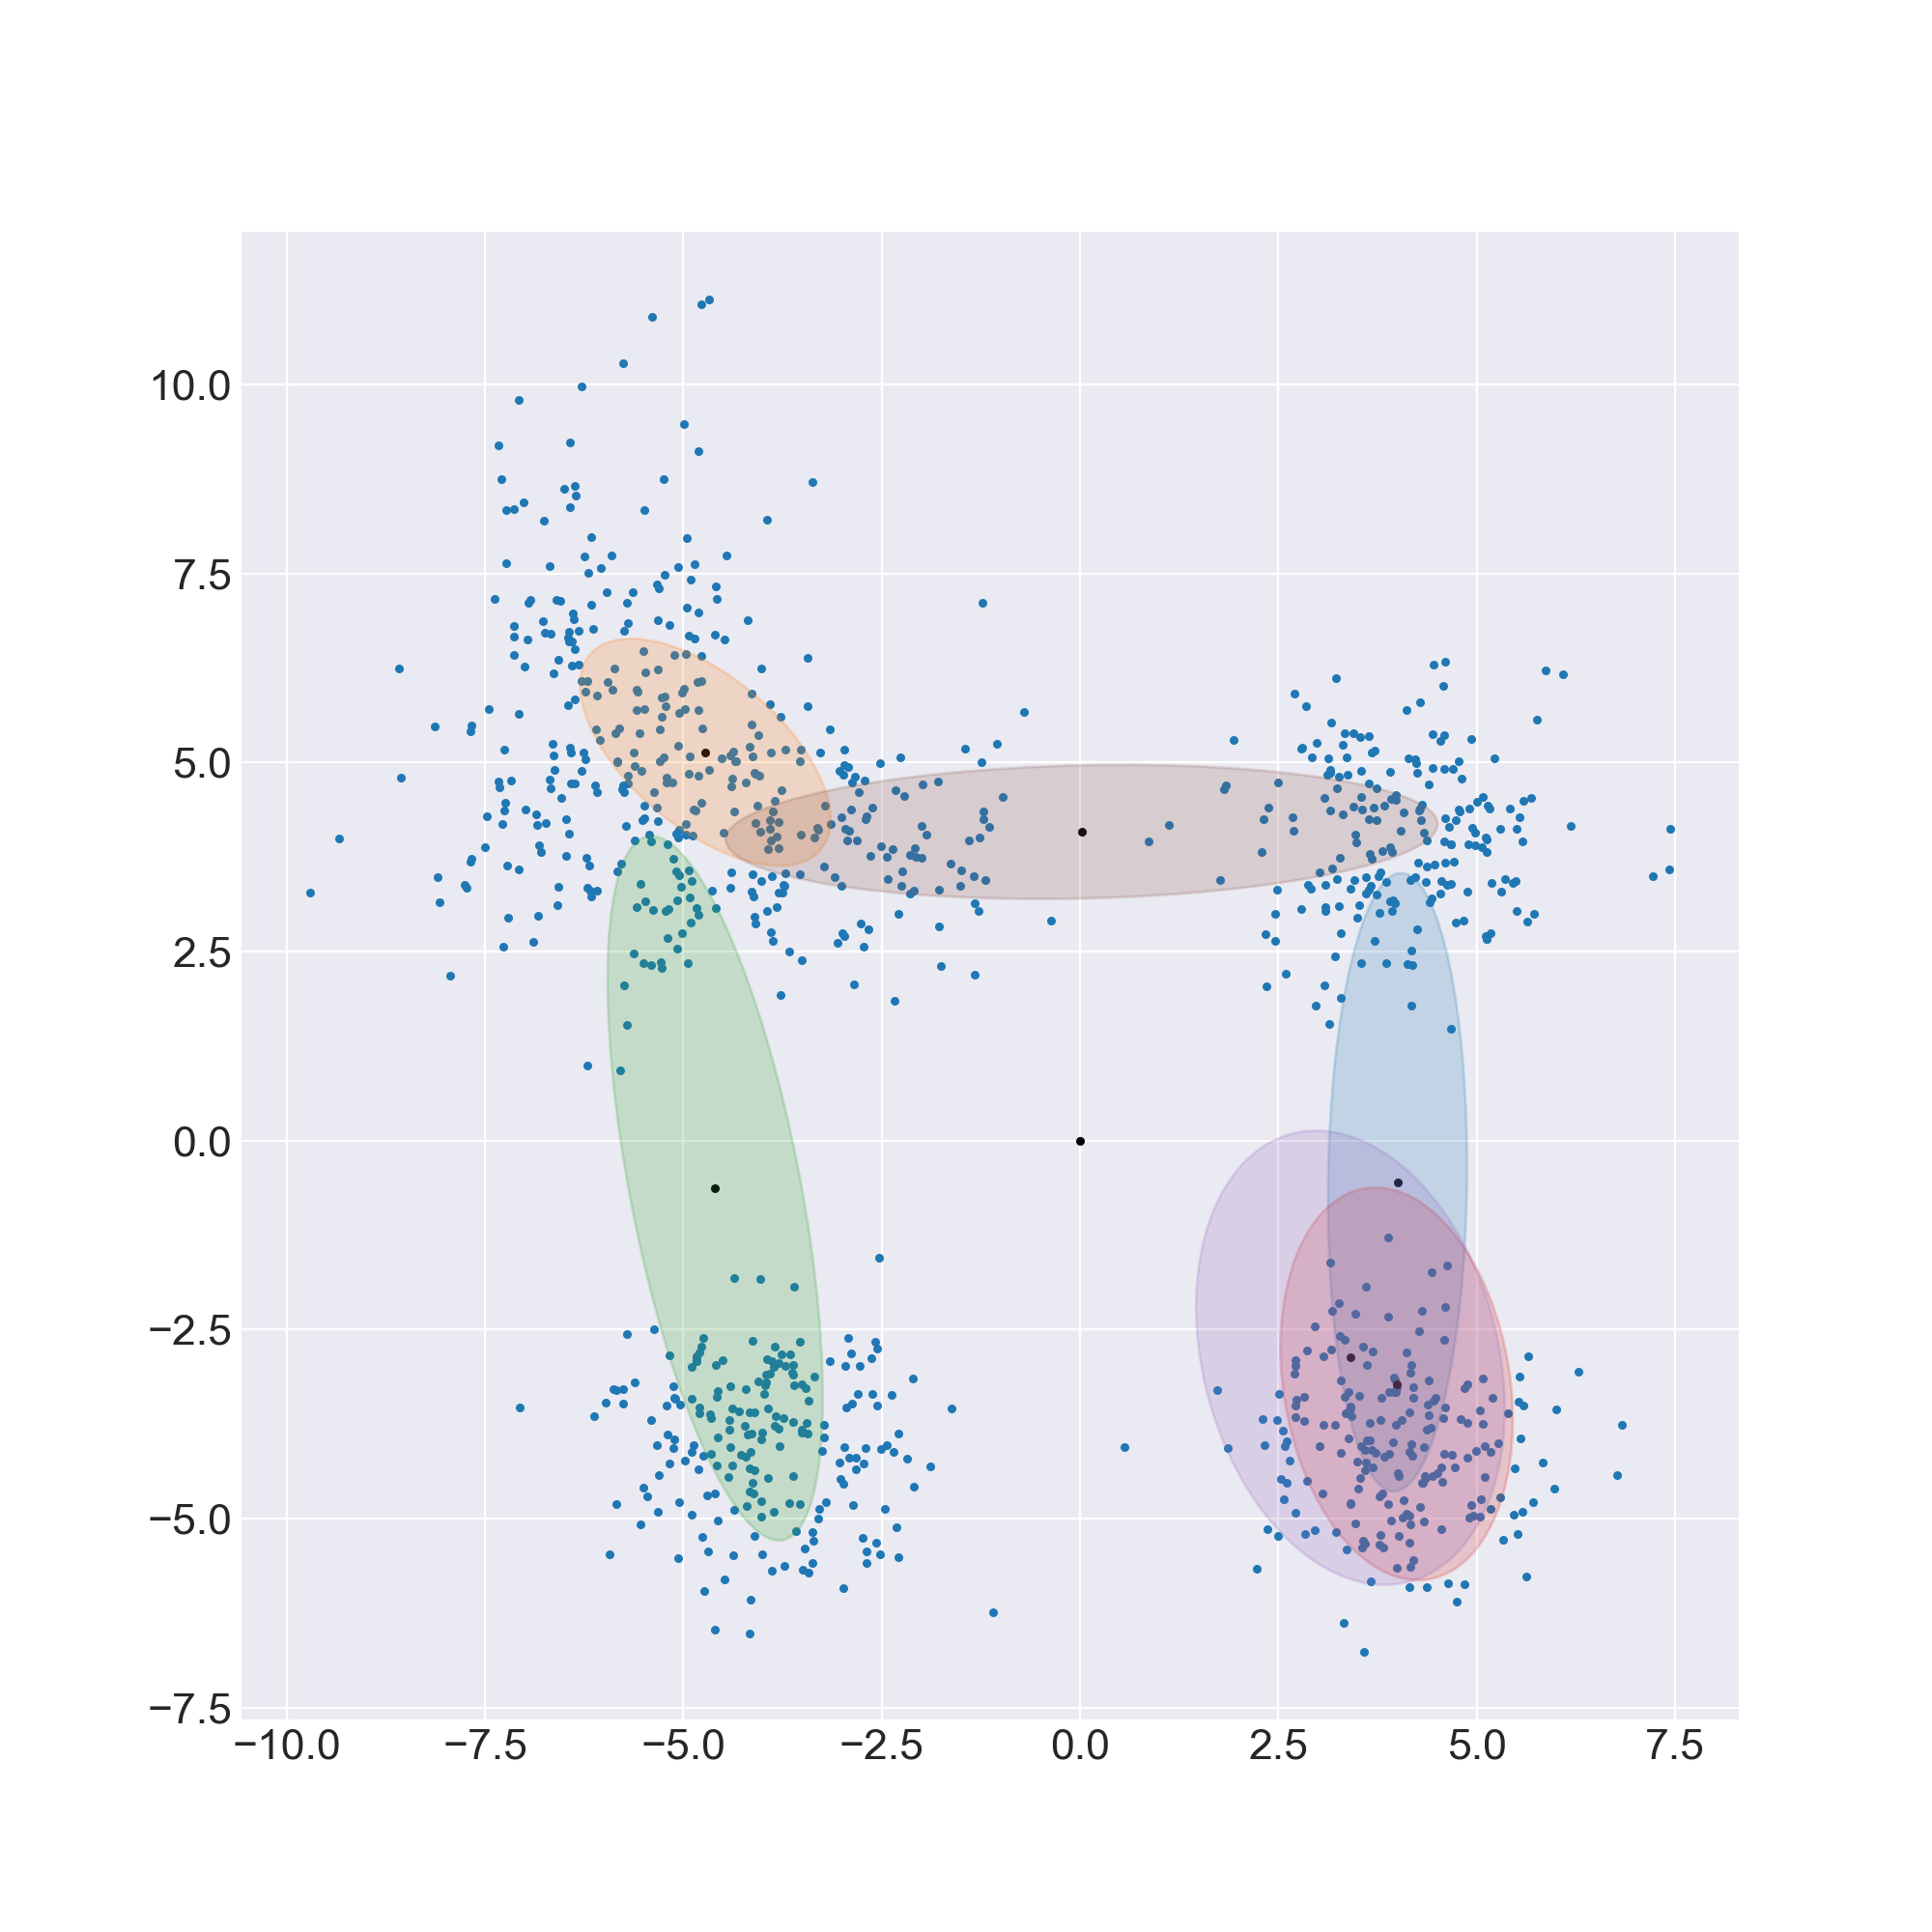
\includegraphics[width=\linewidth]{outputs/simulation/iter_40.png}
    \caption{Iteration 40}
  \end{subfigure}
  \begin{subfigure}[b]{0.22\linewidth}
    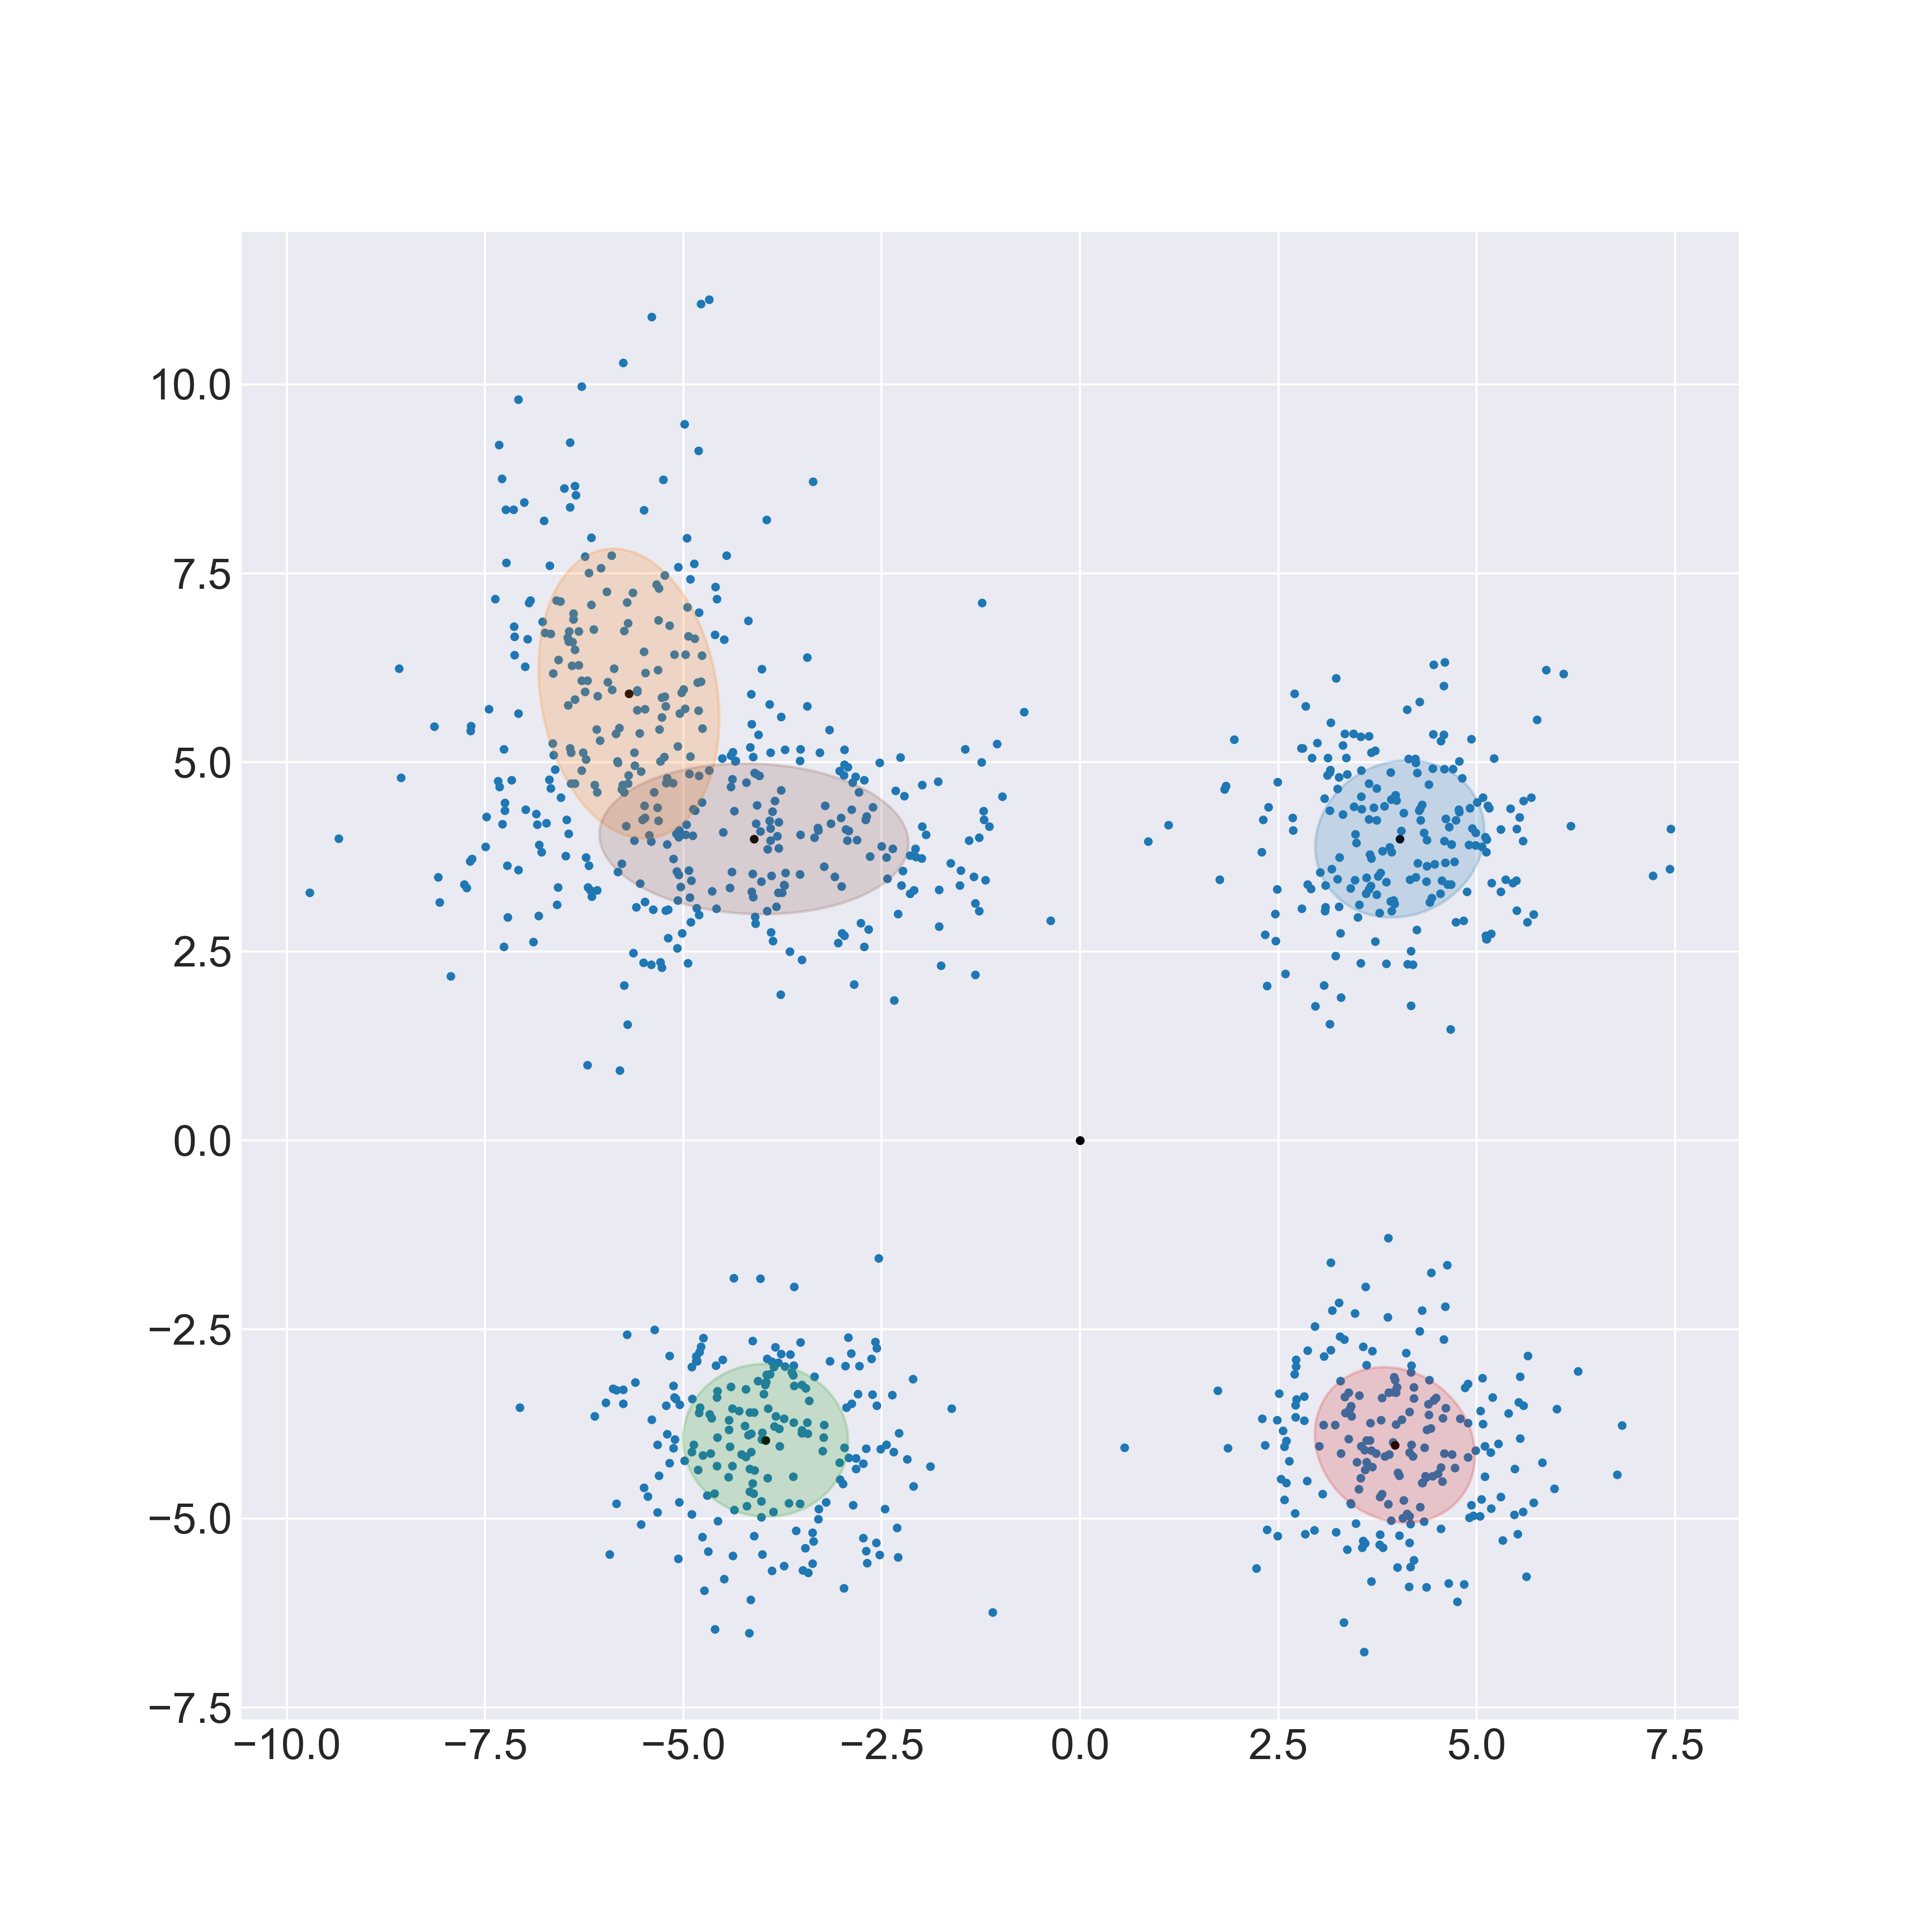
\includegraphics[width=\linewidth]{outputs/simulation/final.png}
    \caption{Converged}
  \end{subfigure}
  \caption{Apply CAVI on a simulated two dimensional mixture of Gaussians training. The figure (a) shows the original data, where we created 5 Gaussians with different mean vectors and covariance matrices. The ellipses are 1$\sigma$ contours of estimated covariance matrices.}
%  \label{fig:coffee3}
\end{figure}
\begin{figure}[H]
  \centering
  \begin{subfigure}[b]{0.45\linewidth}
    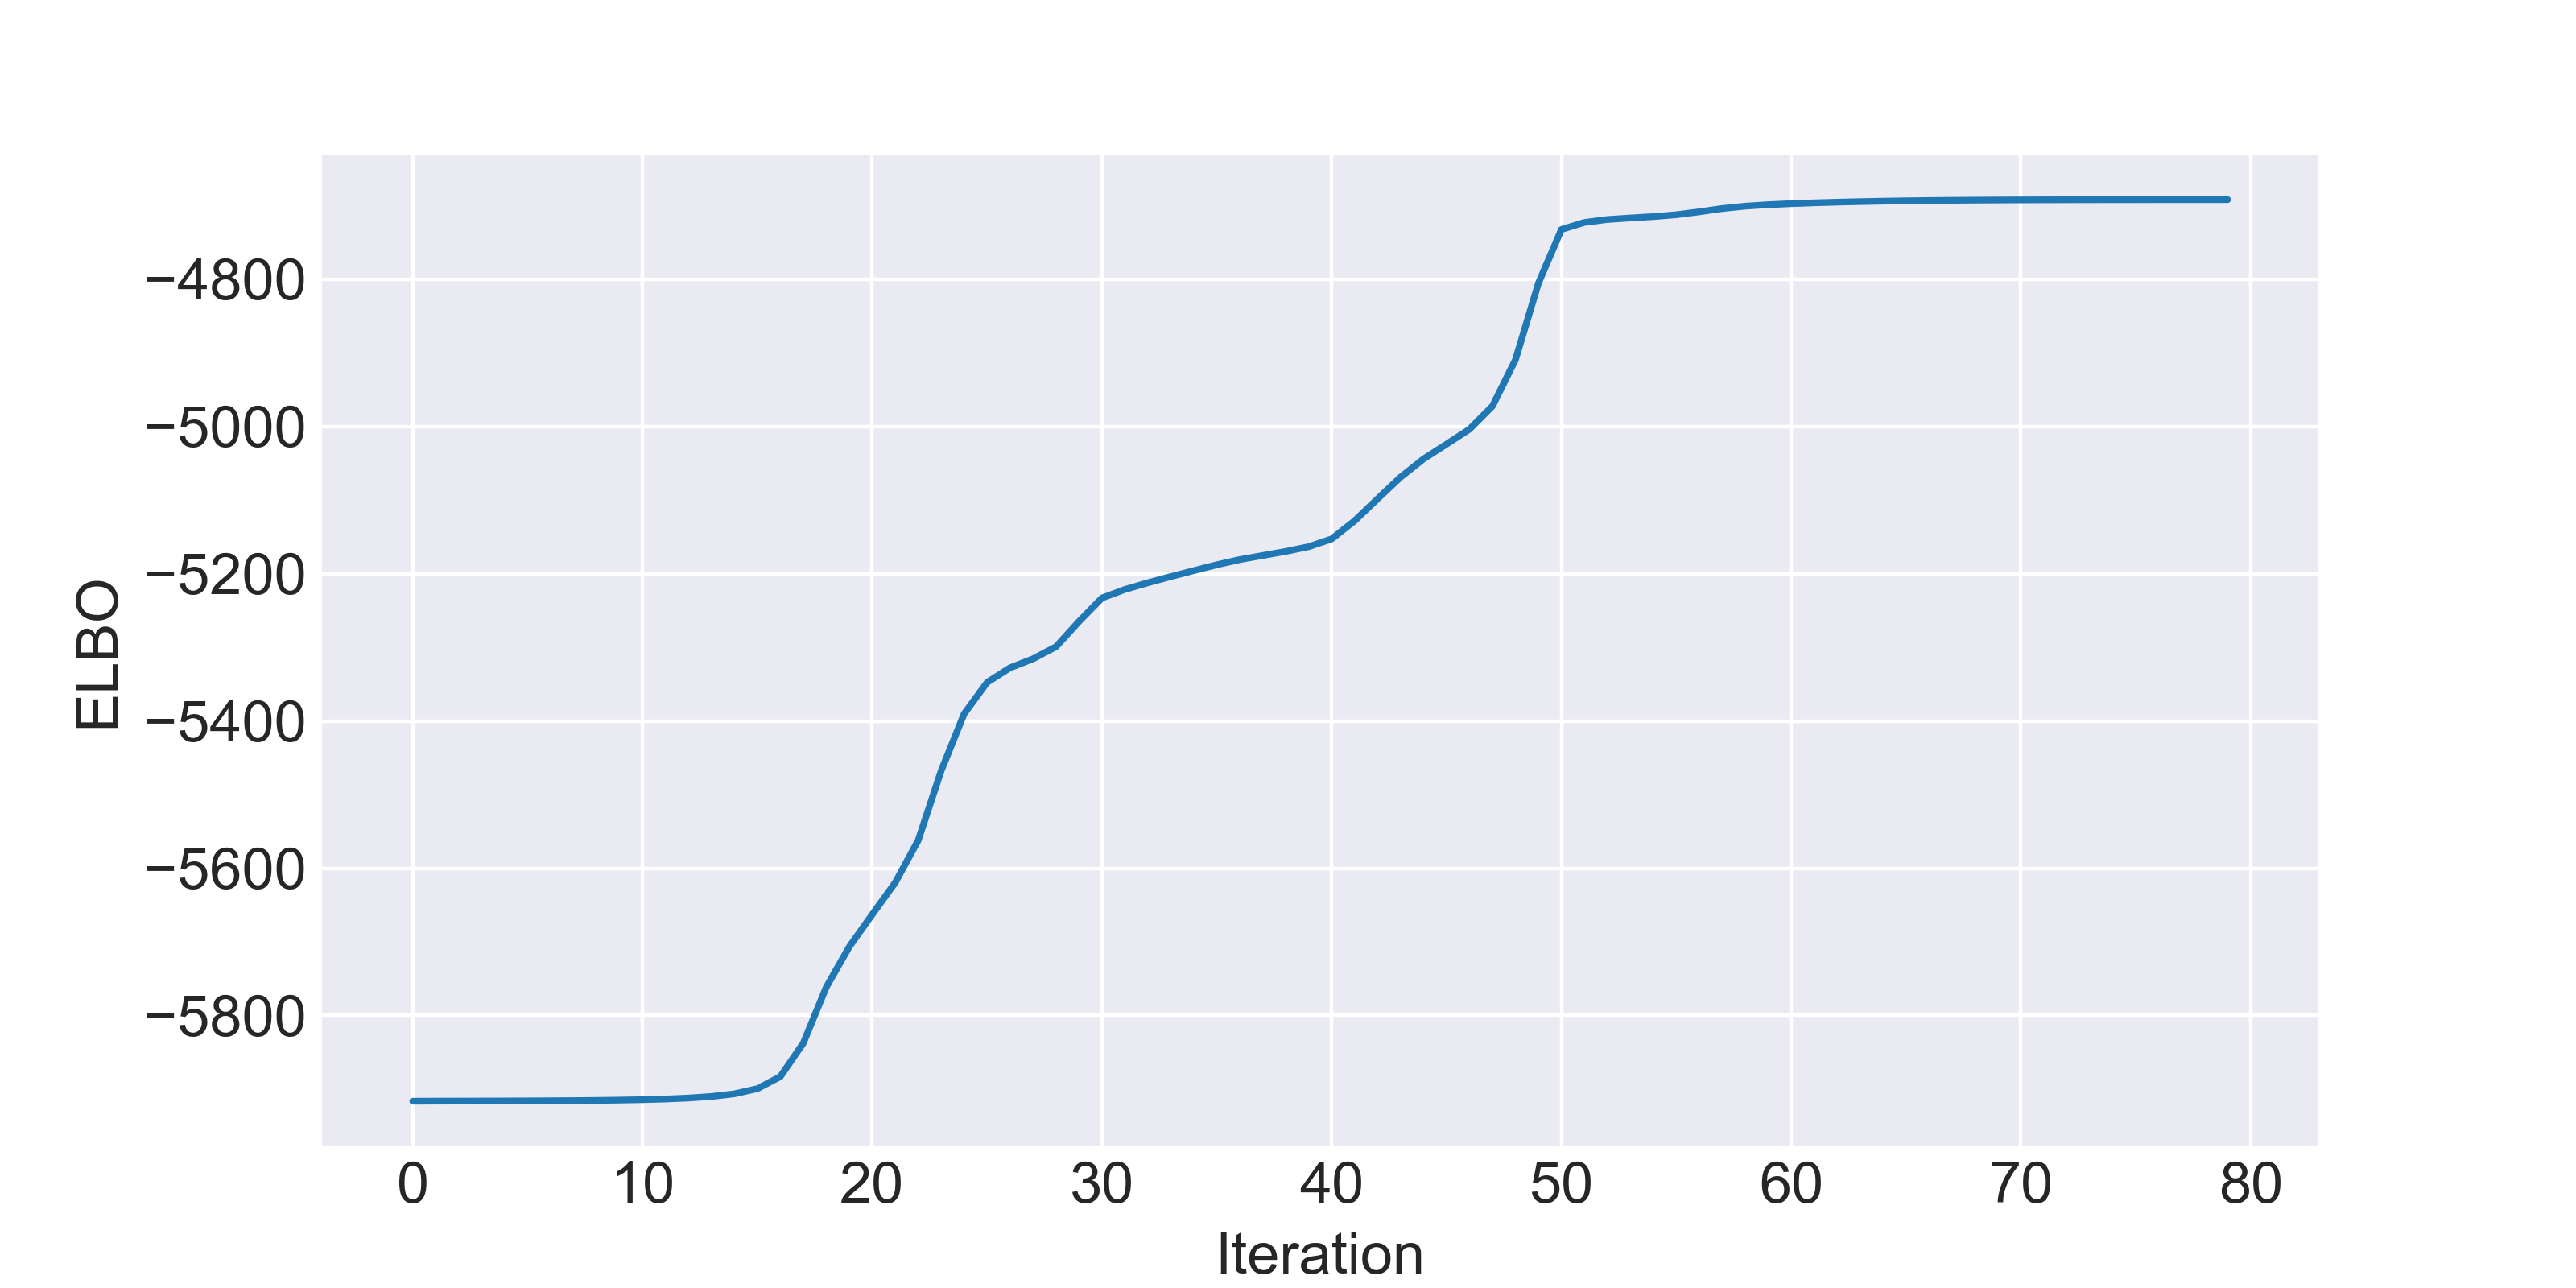
\includegraphics[width=\linewidth]{outputs/simulation/elbo.png}
     \caption{ELBO}
  \end{subfigure}
  \begin{subfigure}[b]{0.45\linewidth}
    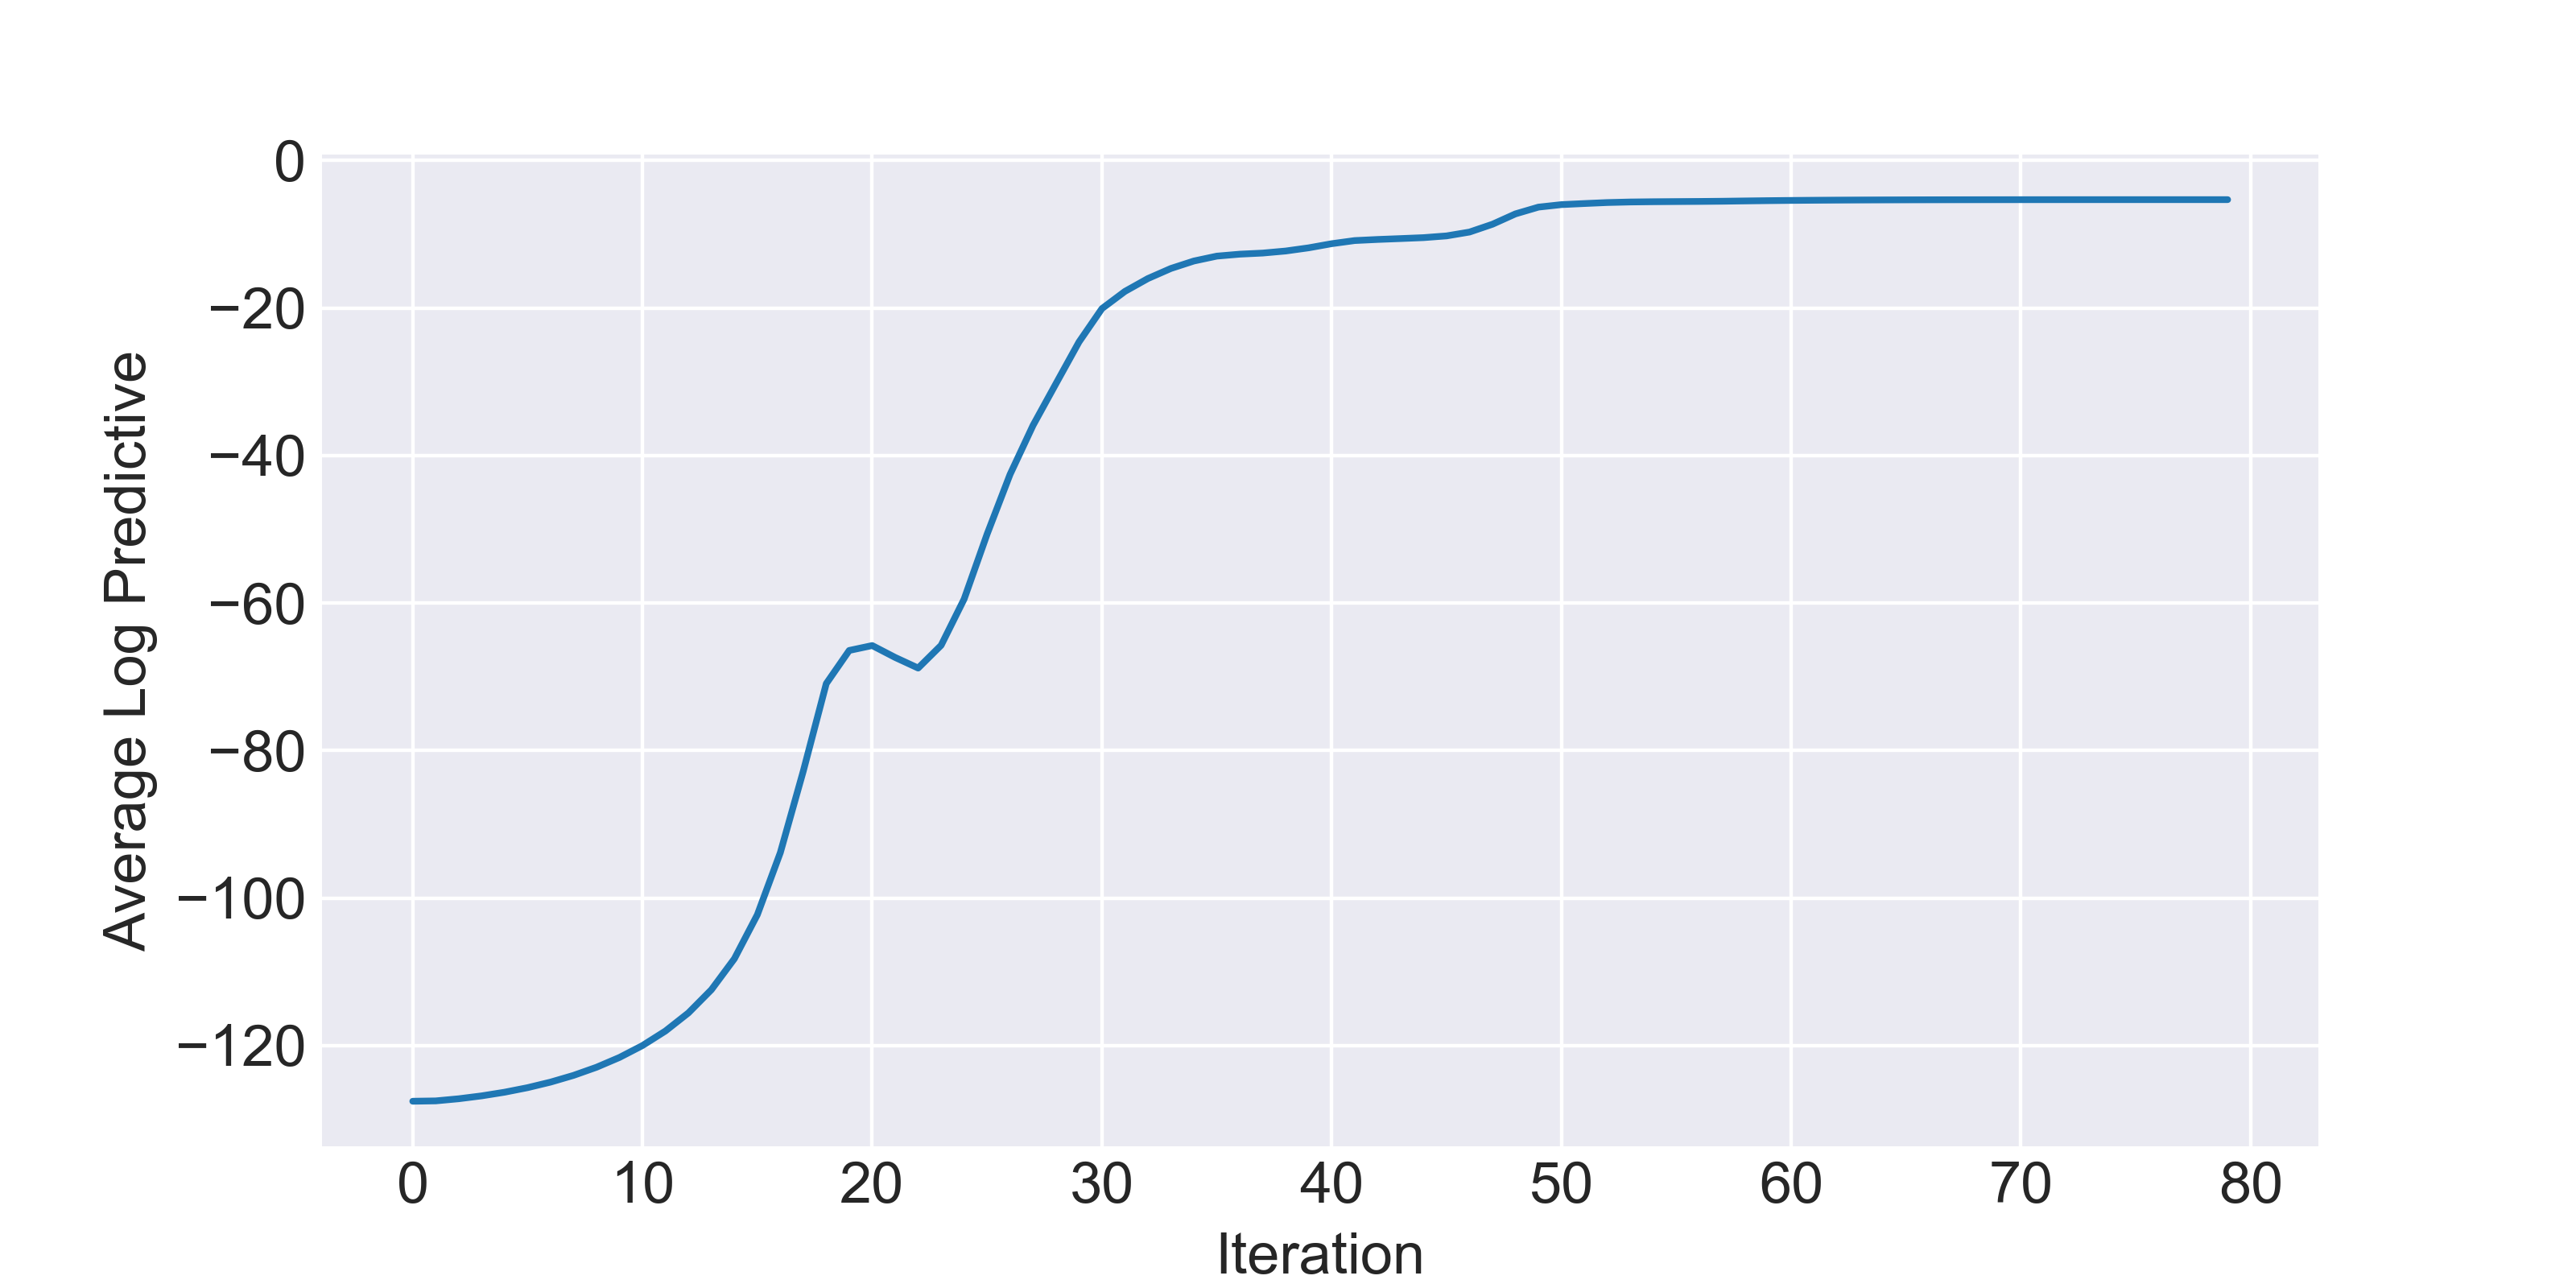
\includegraphics[width=\linewidth]{outputs/simulation/pred_density.png}
    \caption{Average Log Predictive}
  \end{subfigure}
  \caption{The figure (a) shows successive improvement on the evidence lower bound while the figure (b) shows the average of the log predictive calculated on the simulated testing dataset.}
%  \label{fig:coffee3}
\end{figure}

\subsection{Old Faithful dataset}

The Old Faithful dataset describes the waiting time between eruptions and the duration of the eruption for the Old Faithful geyser in Yellowstone National Park. It's a data frame with 272 observations on 2 variables, one is eruption time in mins and one is waiting time to next eruption. The data is plotted in Figure \ref{fig:old1}.

We apply the CAVI algorithm \ref{alg:3} to fit a Gaussian mixture models with 6 clusters to the Old Faithful dataset. Figure \ref{fig:old1} shows the variational density of the components as the CAVI algorithm processes. We could see after convergence, only two components whose expected mixing coefficient are numerically distinguishable form zero.

\begin{figure}[H]
  \centering
  \begin{subfigure}[b]{0.25\linewidth}
    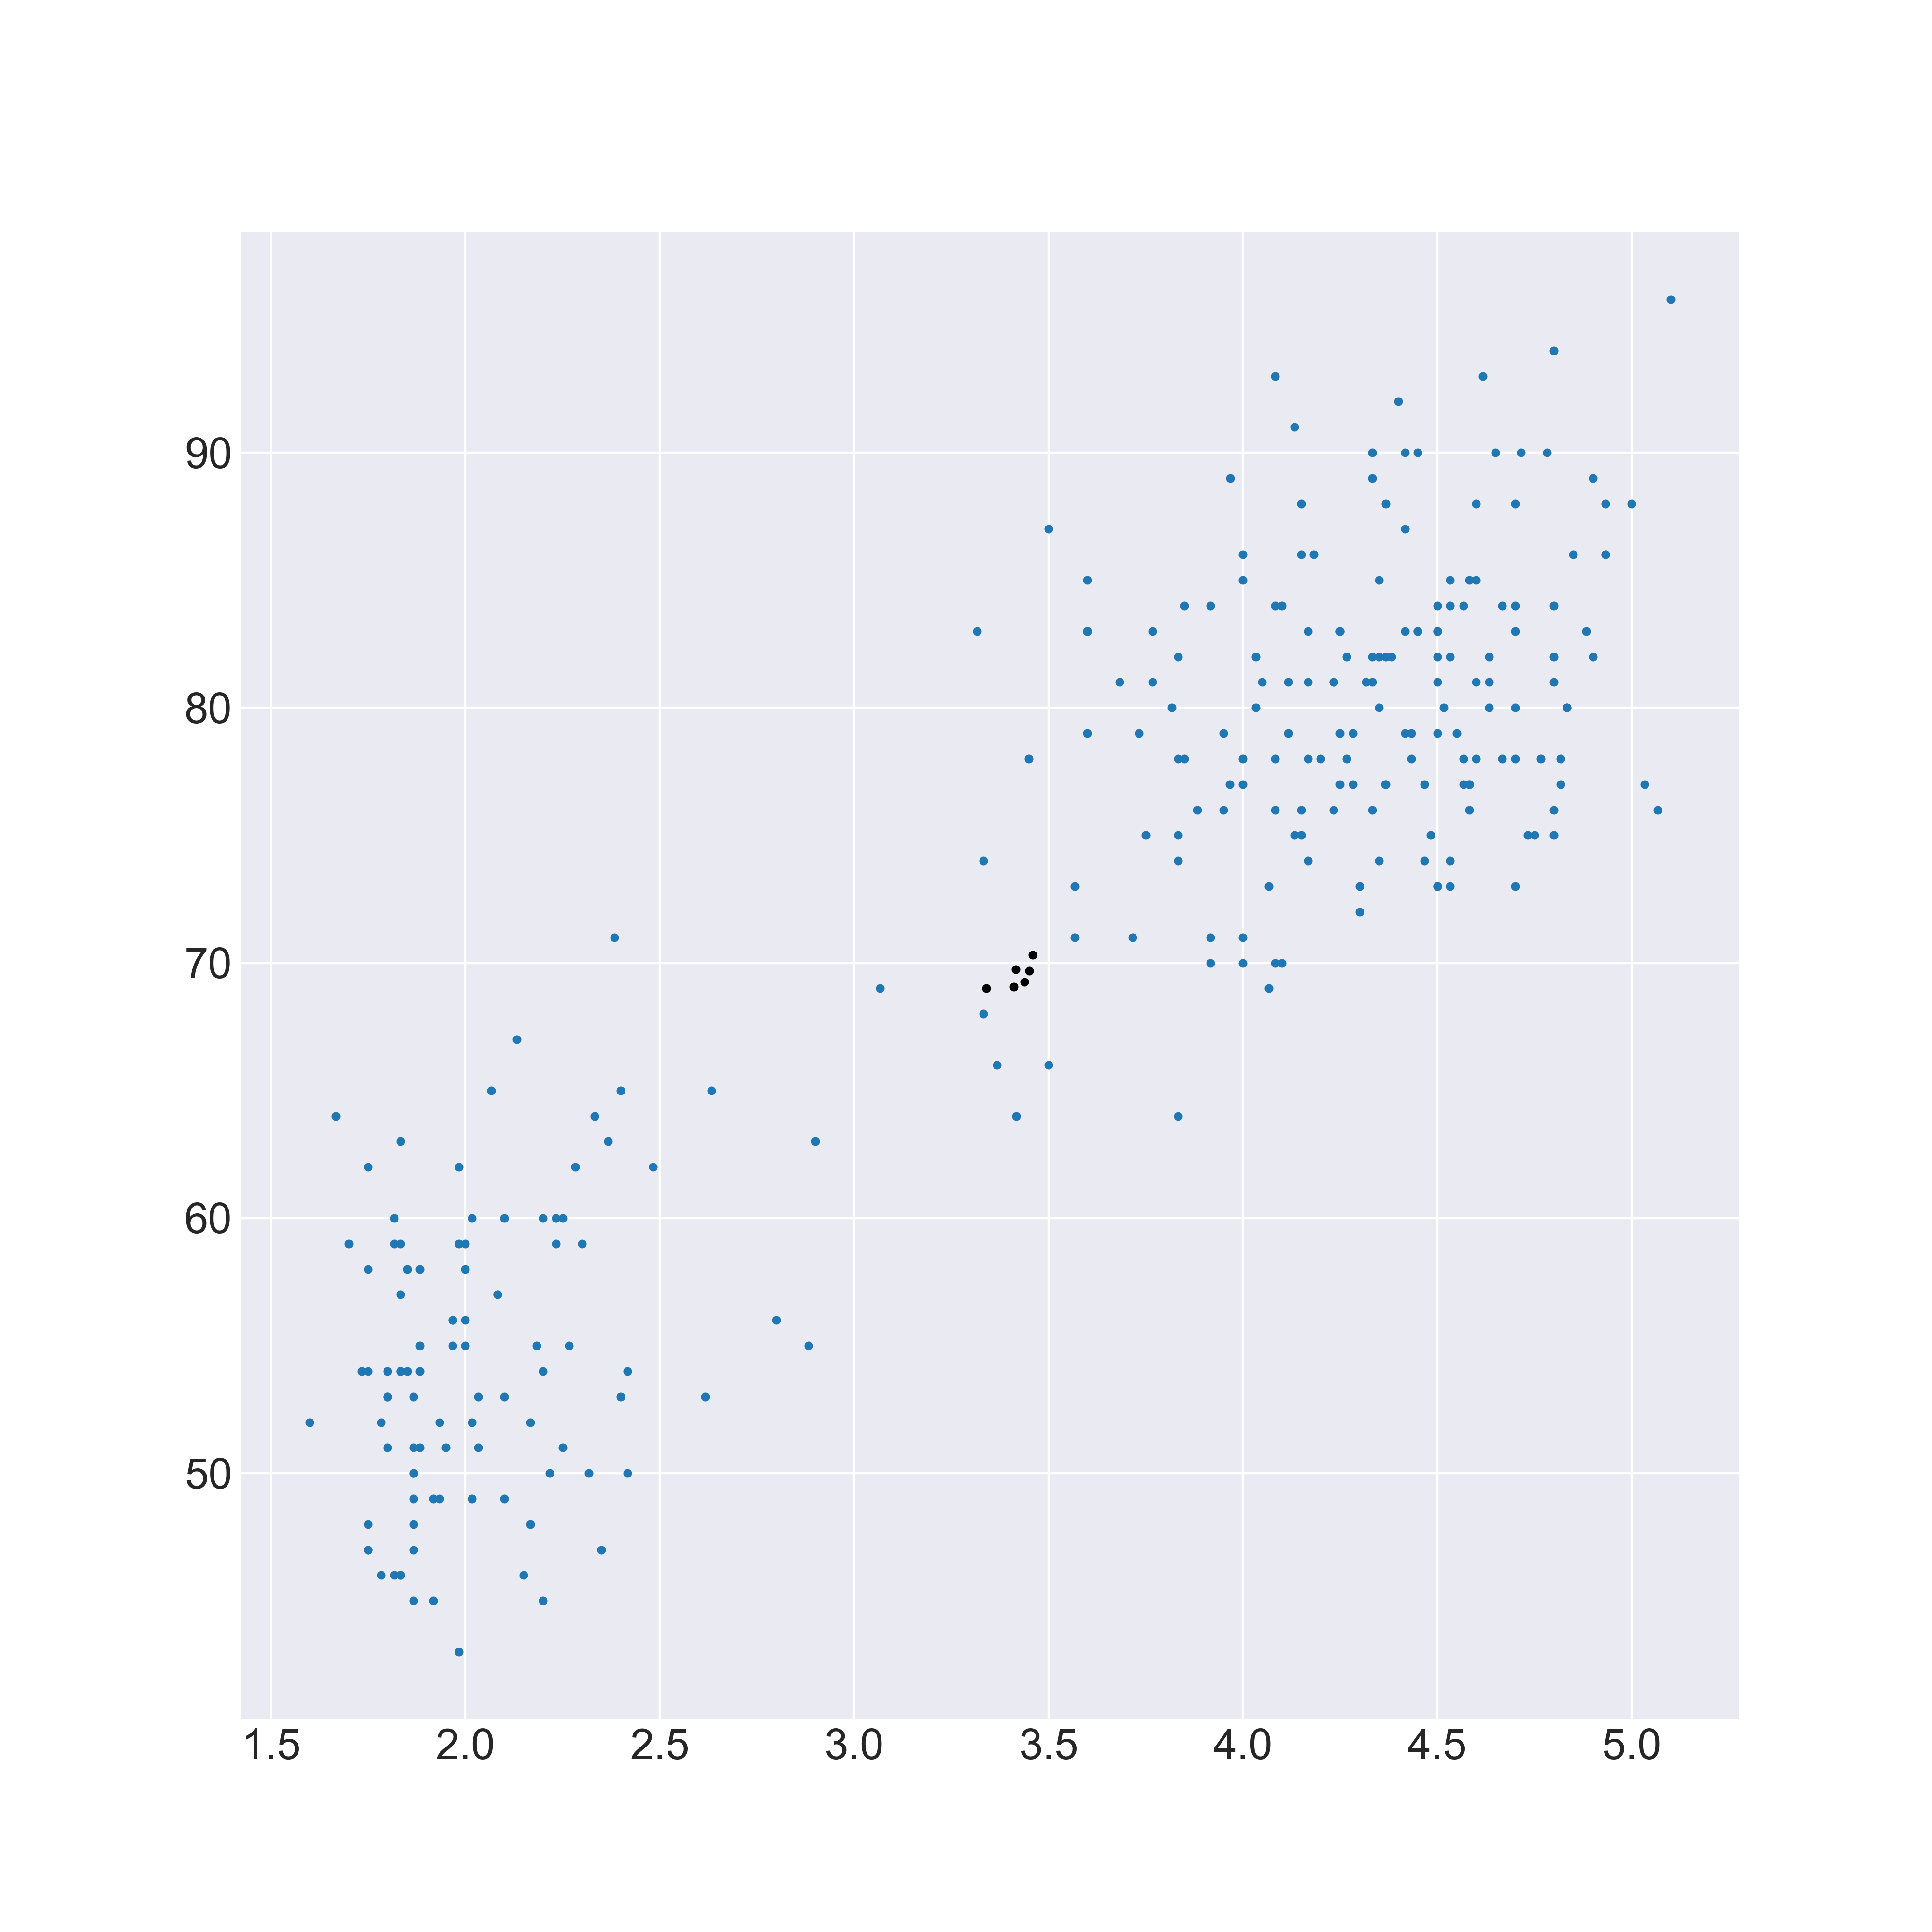
\includegraphics[width=\linewidth]{outputs/old_faithful/iter_0.png}
     \caption{Iteration 0}
  \end{subfigure}
  \begin{subfigure}[b]{0.25\linewidth}
    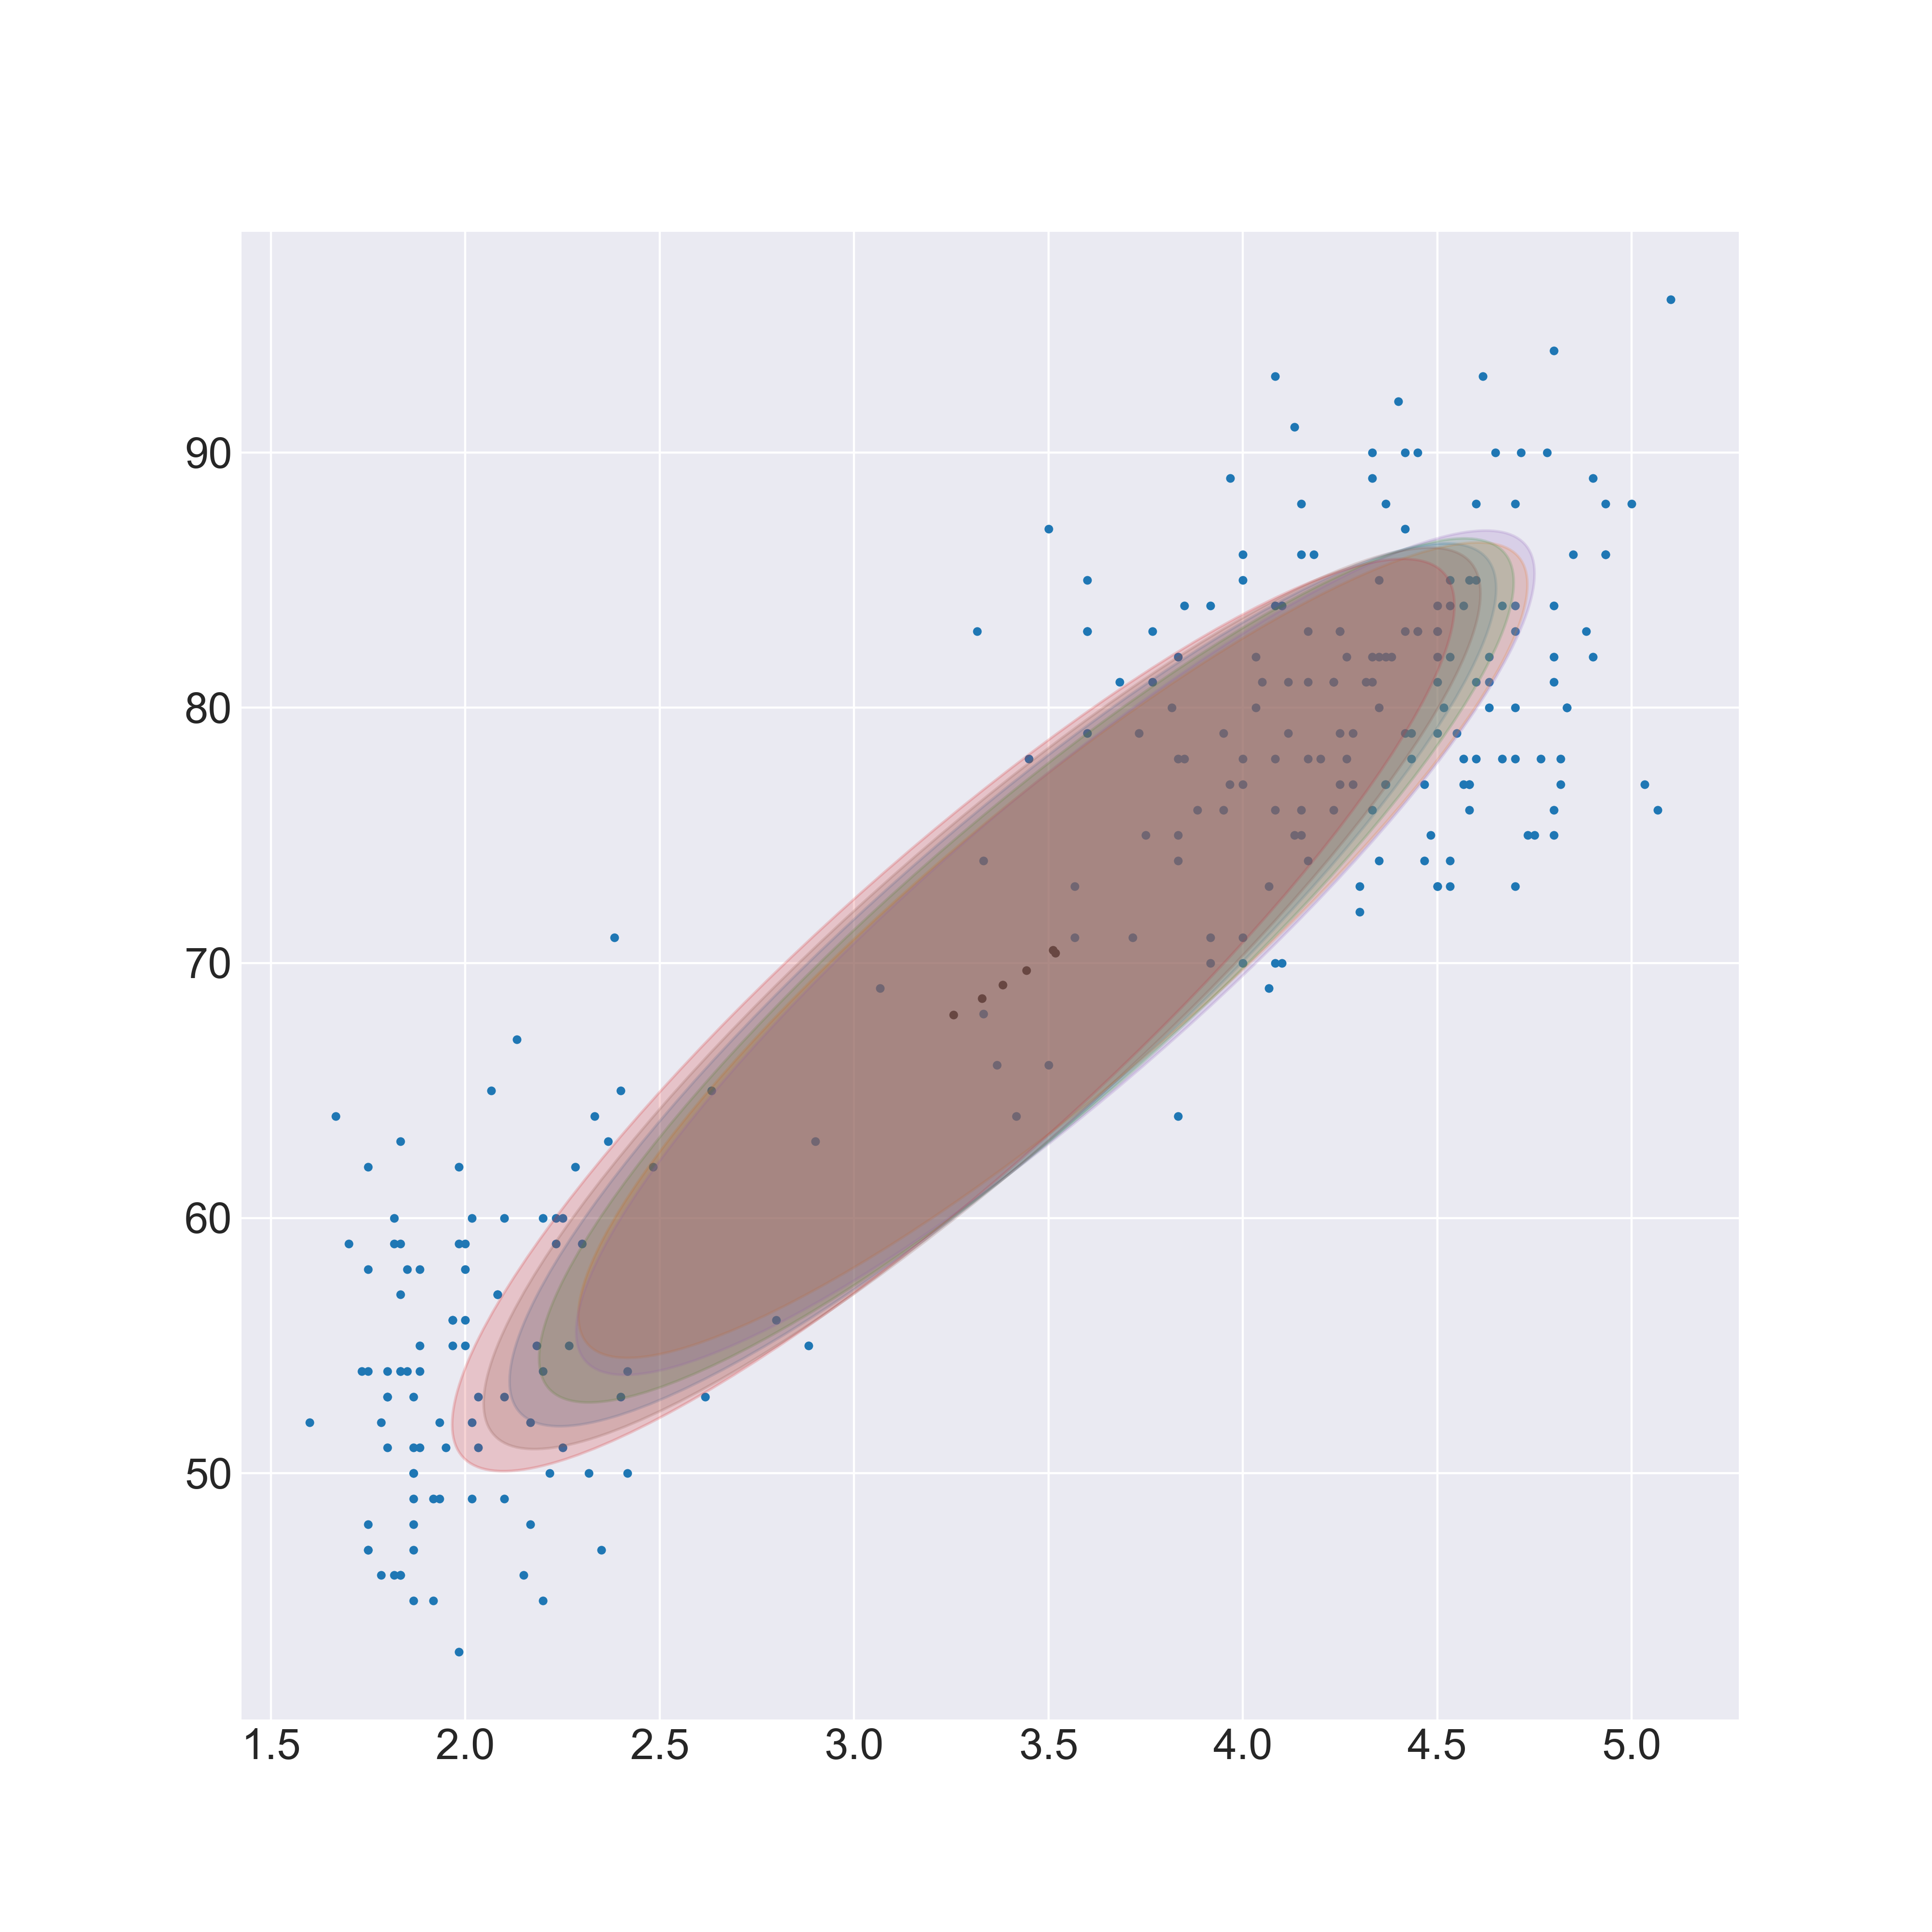
\includegraphics[width=\linewidth]{outputs/old_faithful/iter_10.png}
    \caption{Iteration 10}
  \end{subfigure}
  \begin{subfigure}[b]{0.25\linewidth}
    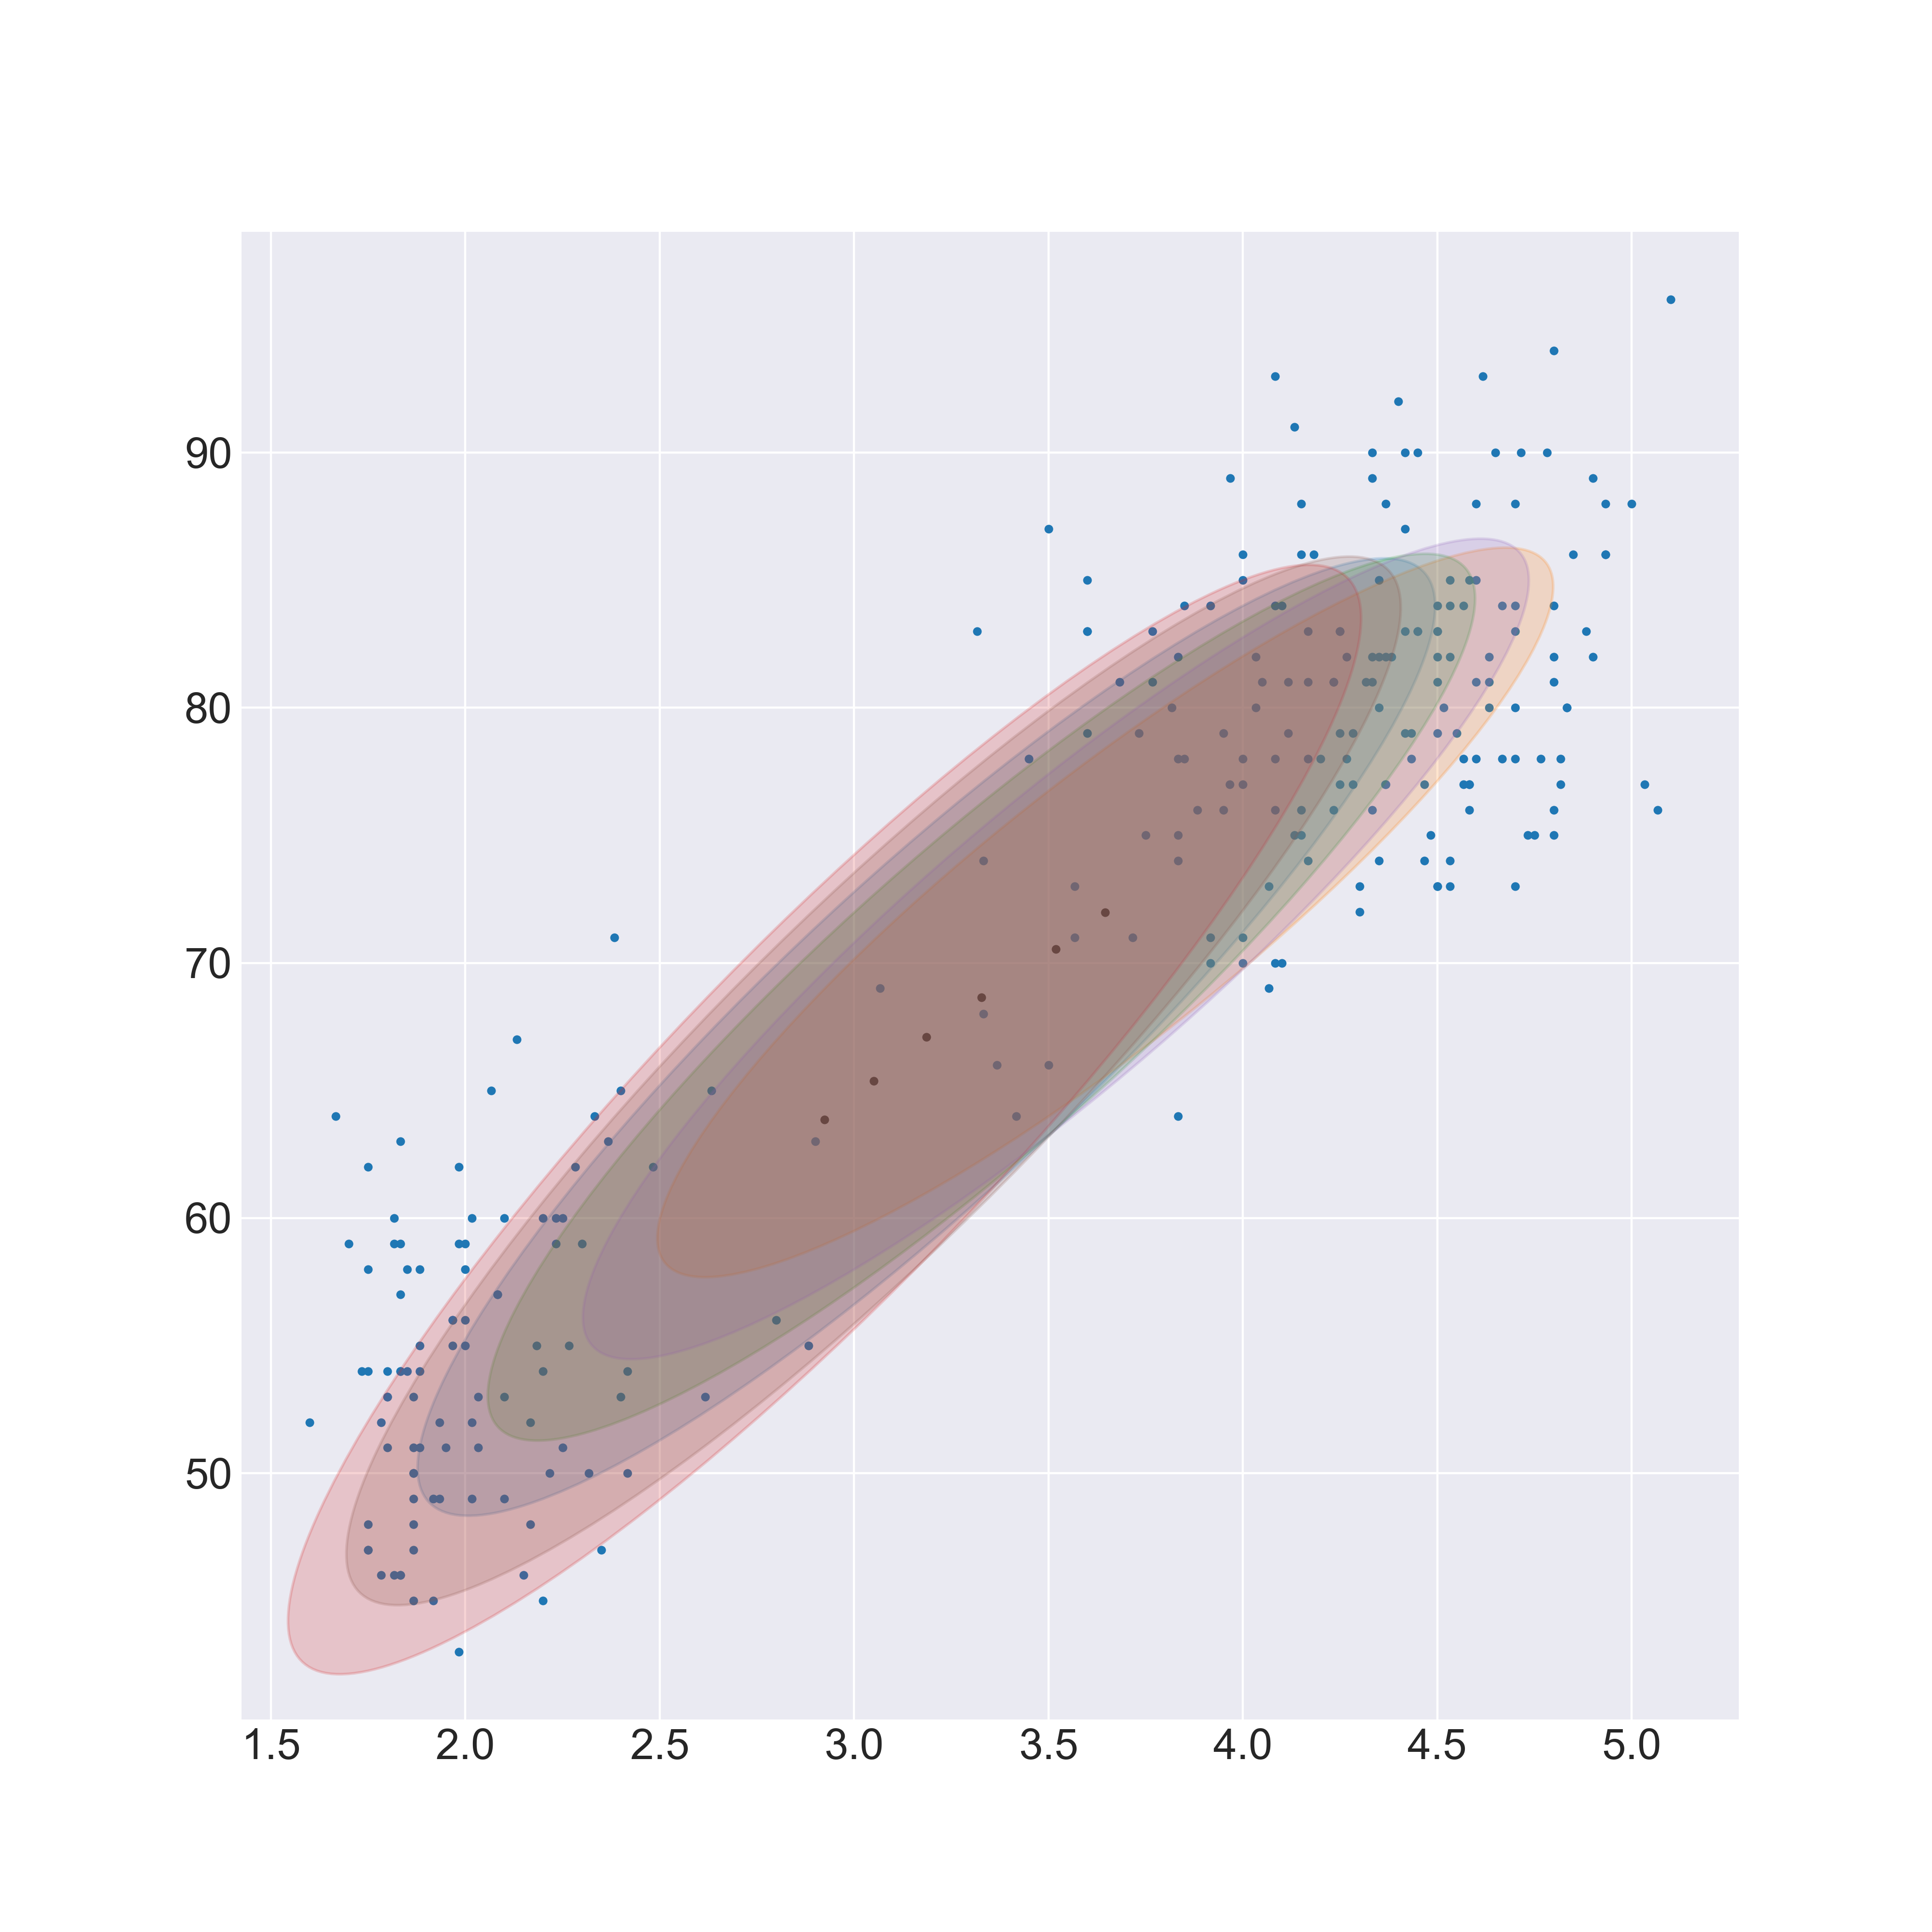
\includegraphics[width=\linewidth]{outputs/old_faithful/iter_20.png}
    \caption{Iteration 20}
  \end{subfigure}
  \begin{subfigure}[b]{0.25\linewidth}
    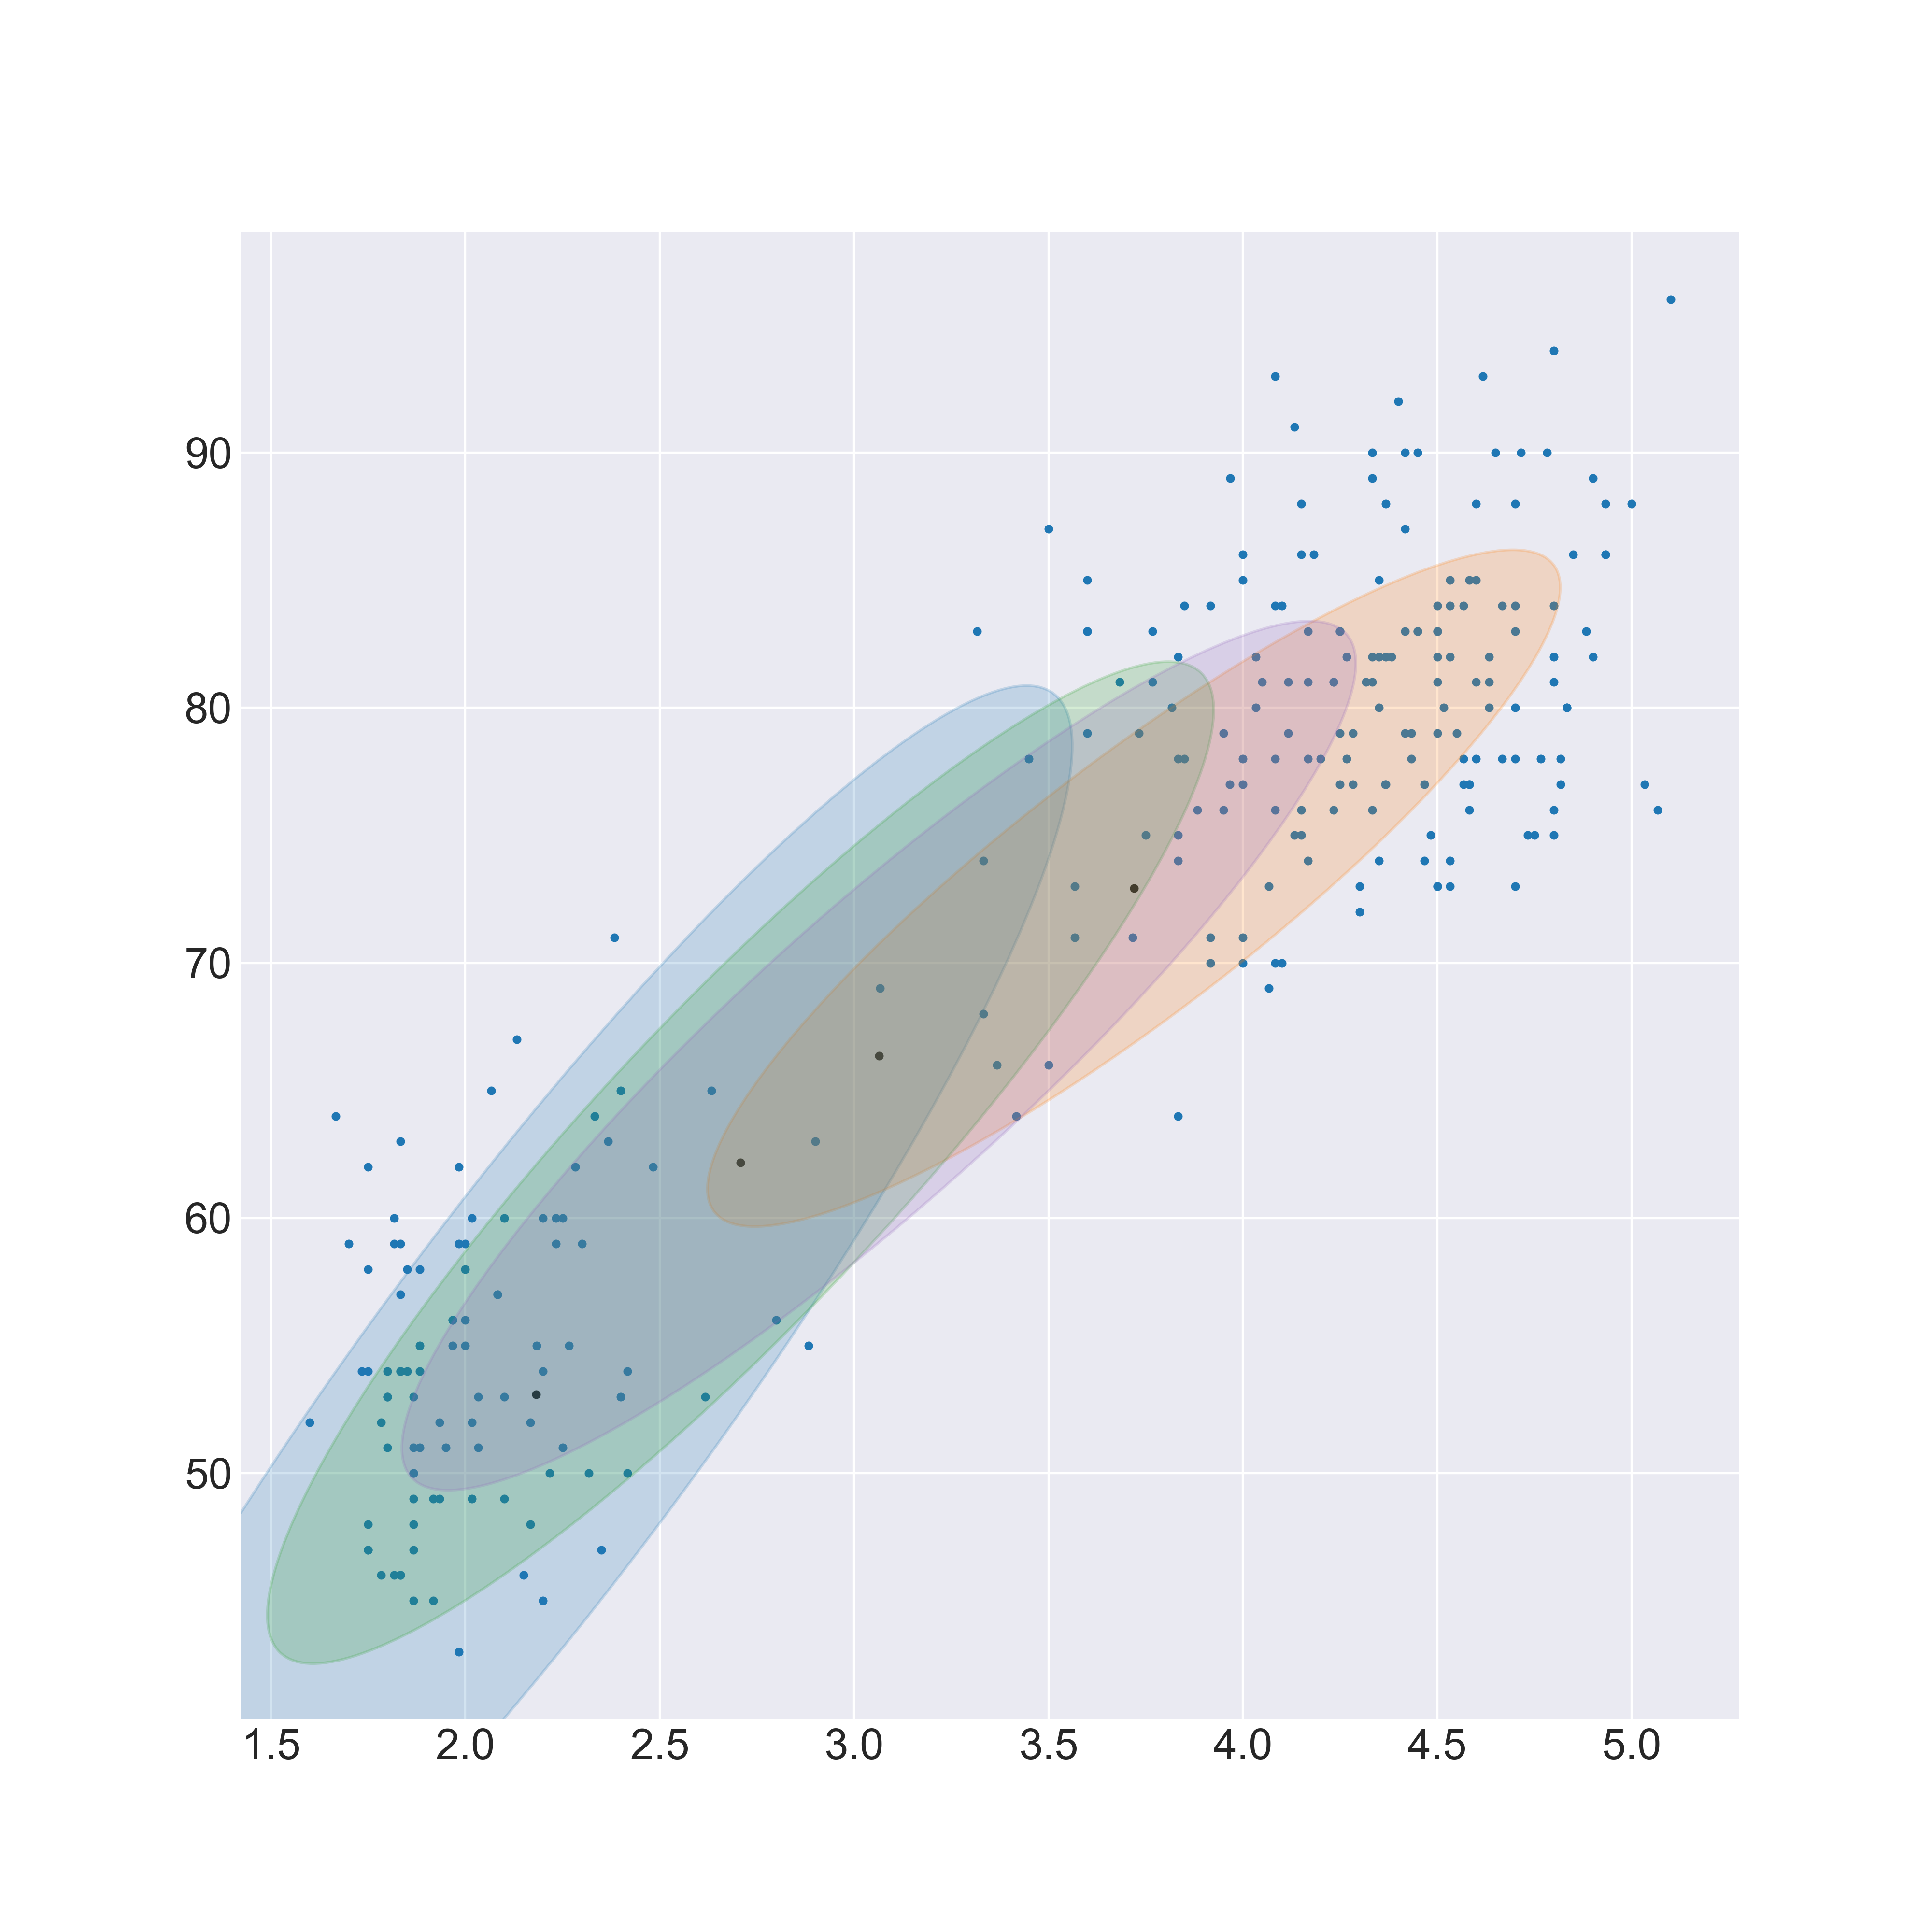
\includegraphics[width=\linewidth]{outputs/old_faithful/iter_30.png}
     \caption{Iteration 30}
  \end{subfigure}
  \begin{subfigure}[b]{0.25\linewidth}
    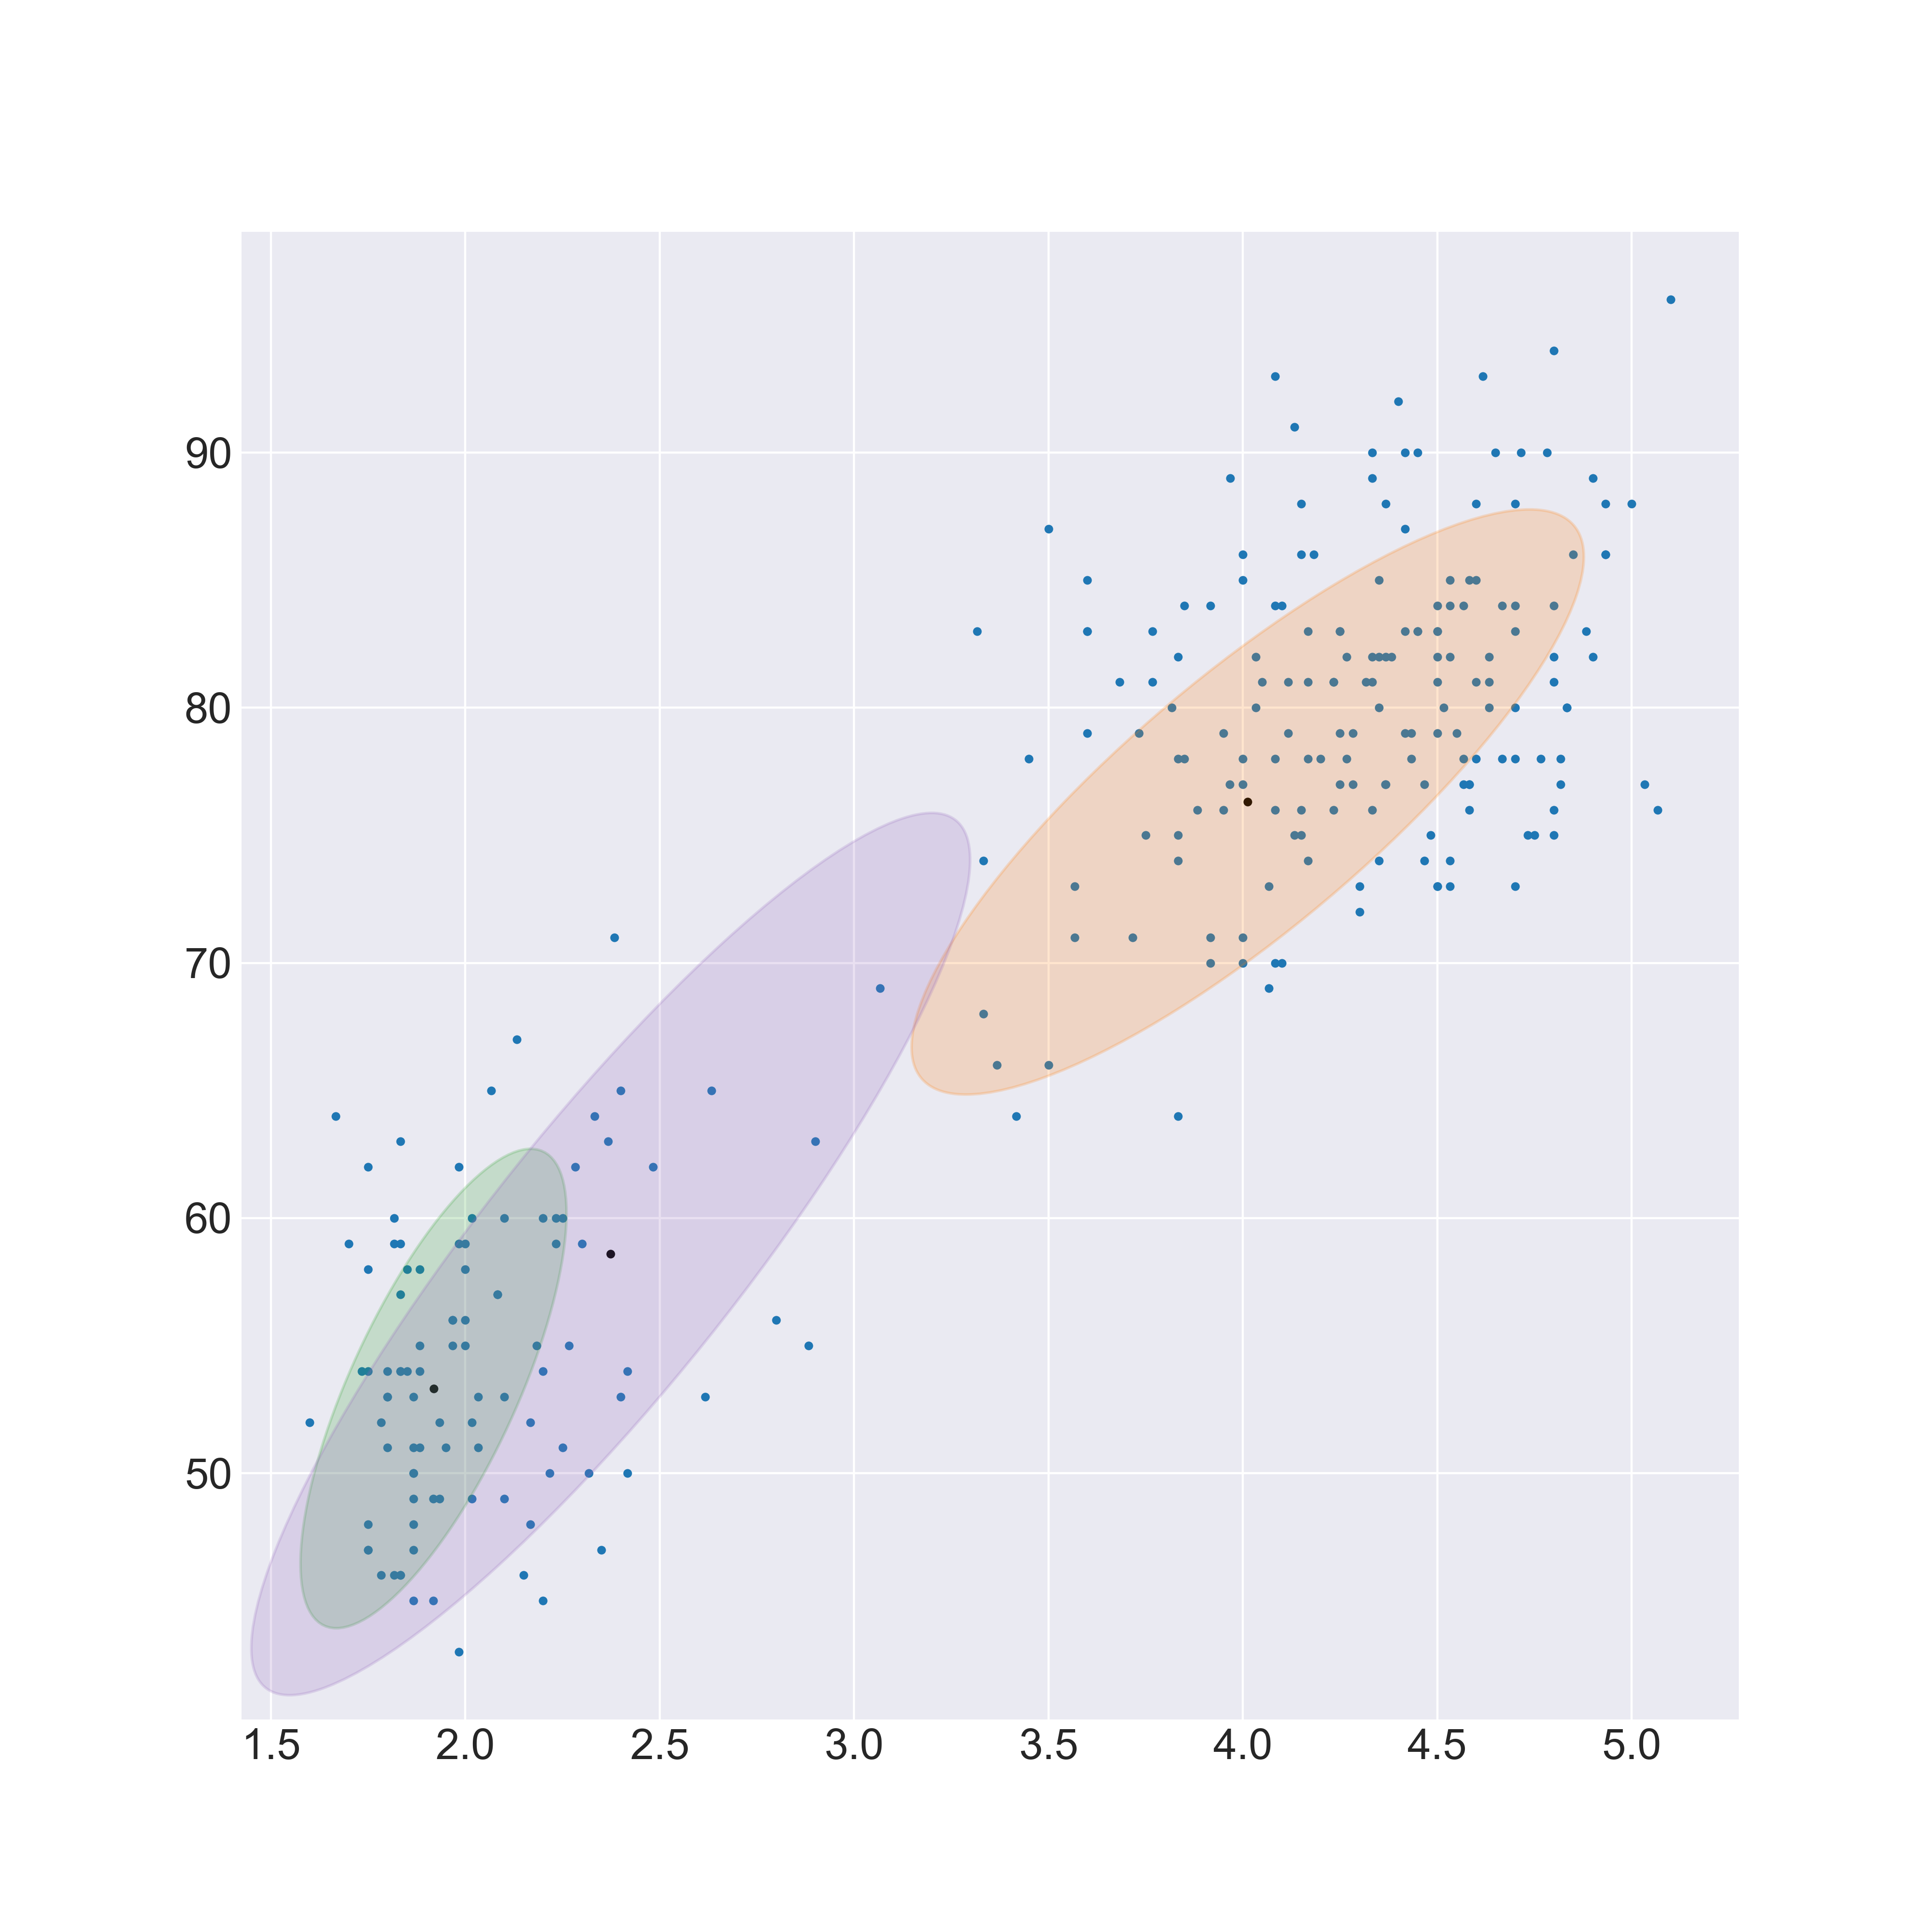
\includegraphics[width=\linewidth]{outputs/old_faithful/iter_40.png}
    \caption{Iteration 40}
  \end{subfigure}
  \begin{subfigure}[b]{0.25\linewidth}
    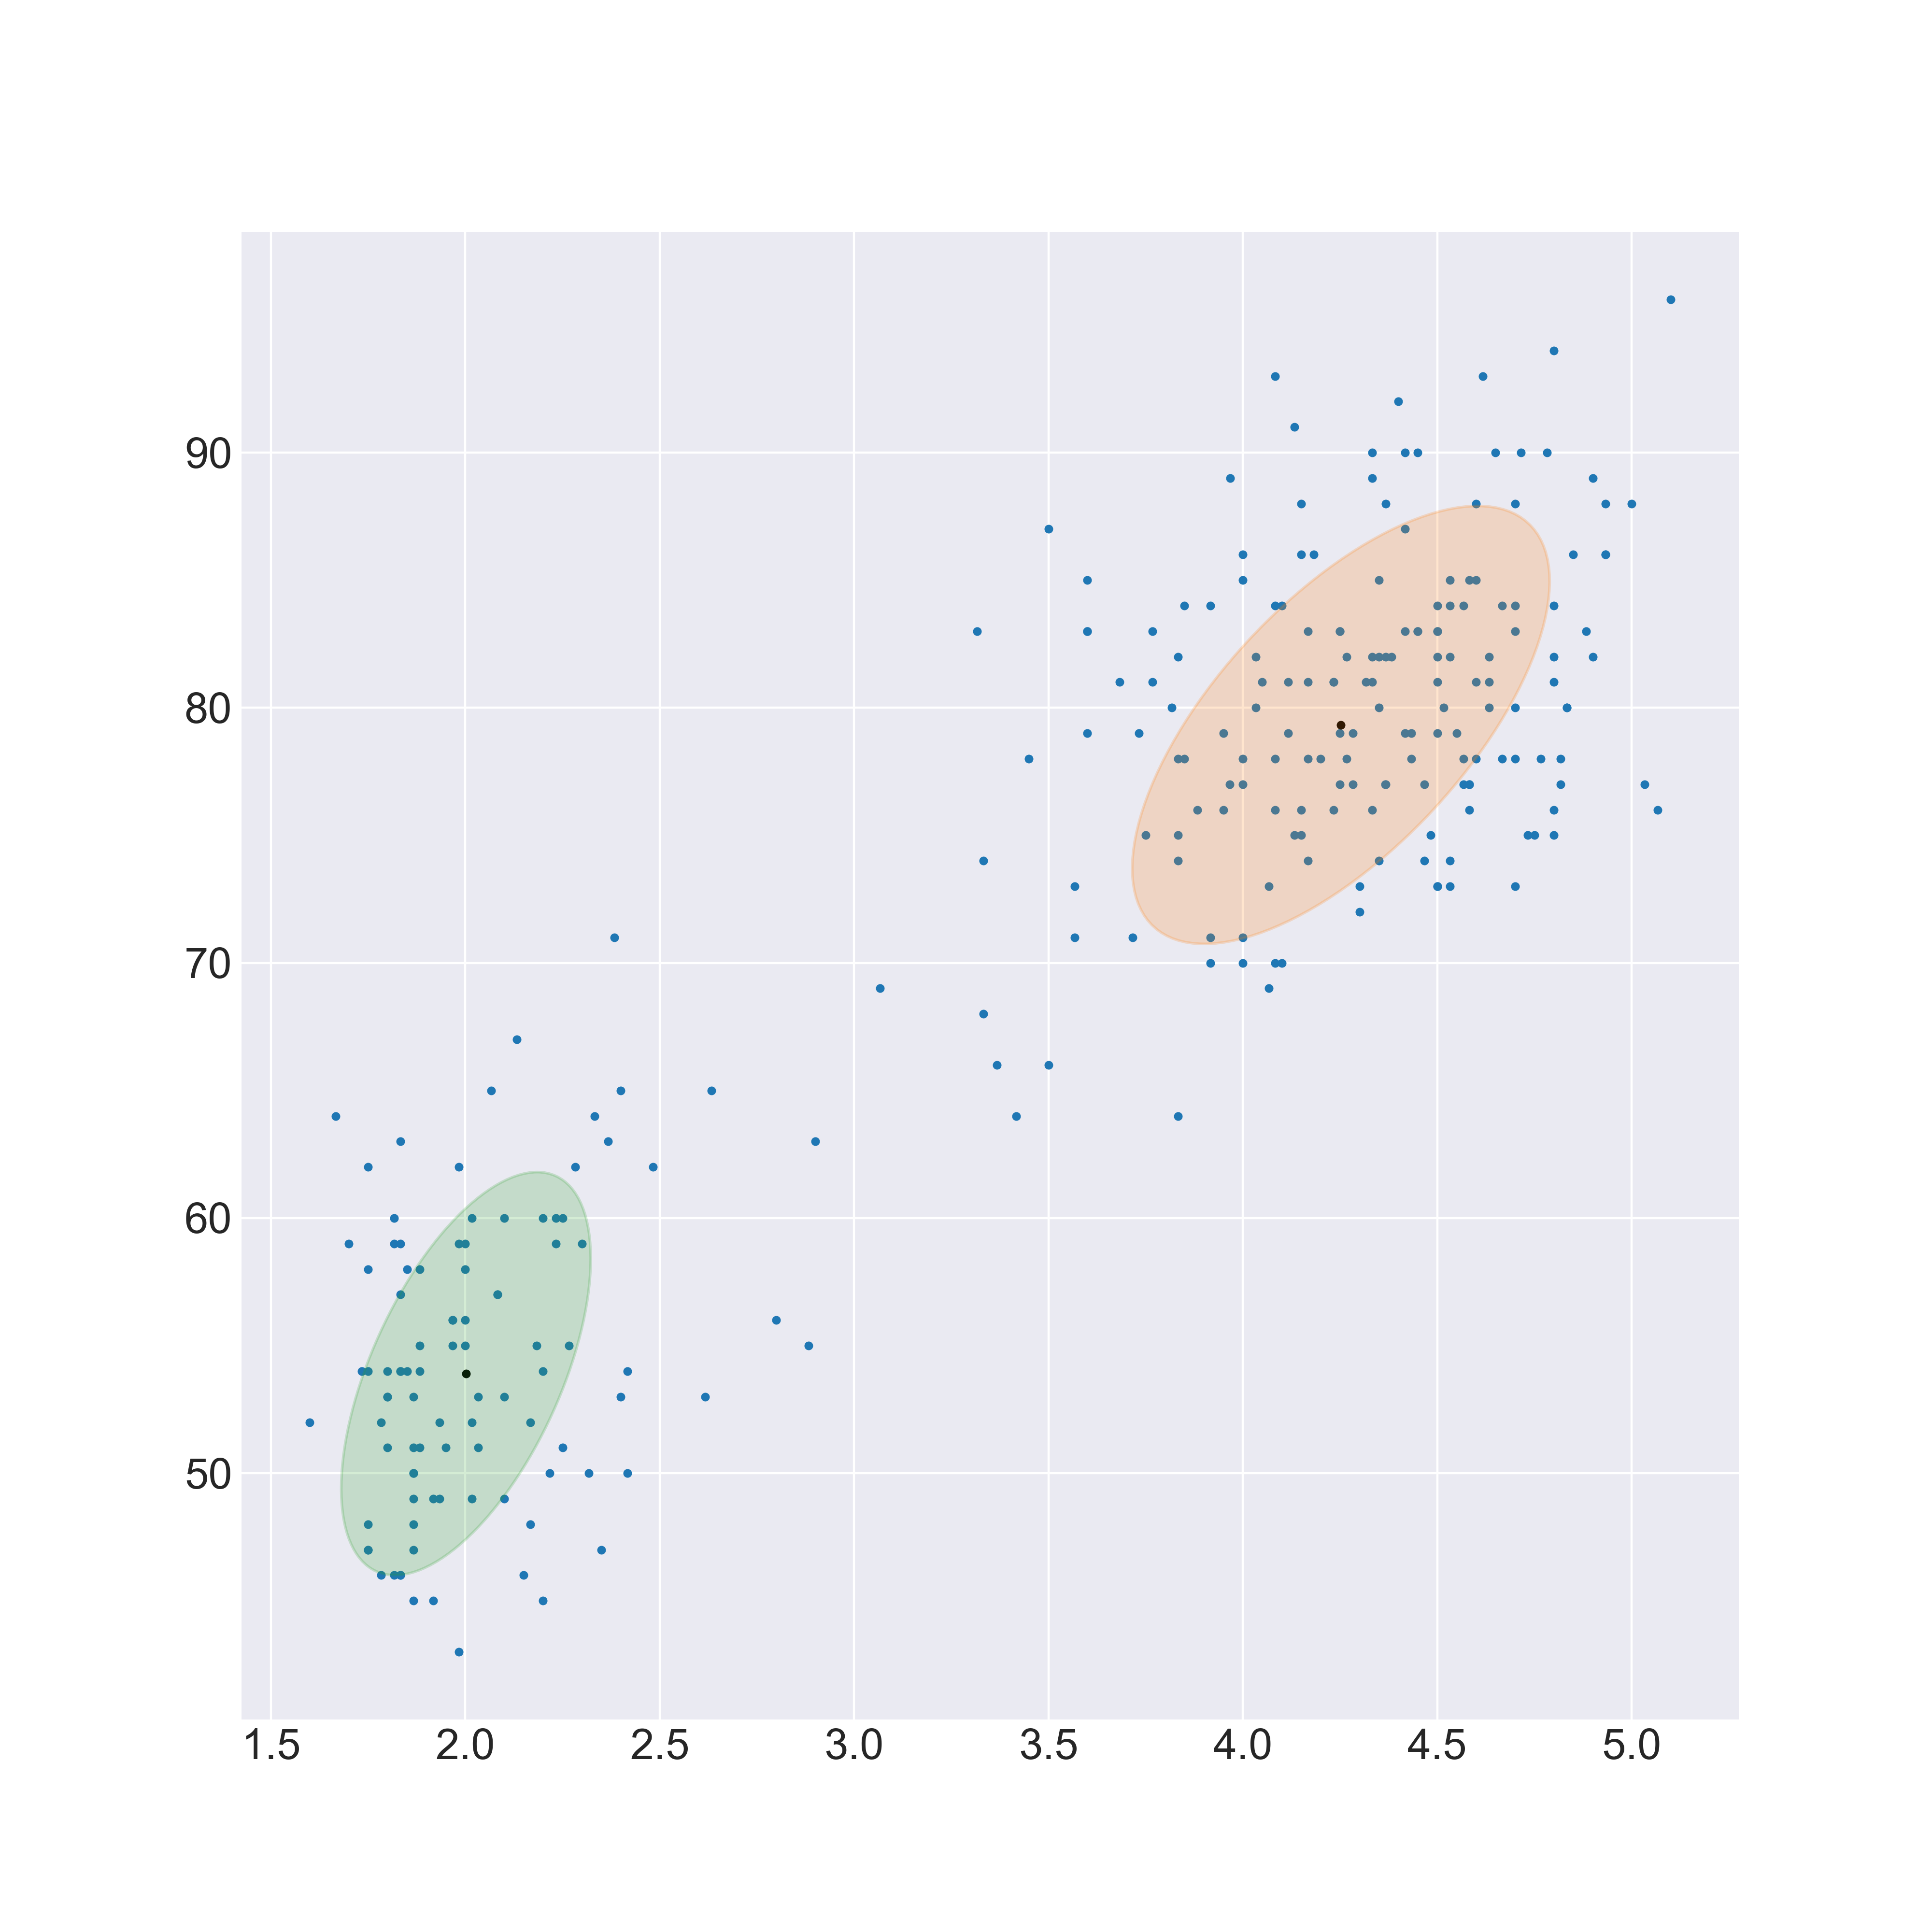
\includegraphics[width=\linewidth]{outputs/old_faithful/final.png}
    \caption{Converged}
  \end{subfigure}
  \caption{Apply CAVI on the old faithful dataset. The ellipses are 1$\sigma$ contours of estimated covariance matrices. Components whose expected mixing coefficient are numerically indistinguishable from zero are not plotted.}
\label{fig:old1}
\end{figure}


\begin{figure}[H]
  \centering
  \begin{subfigure}[b]{0.45\linewidth}
    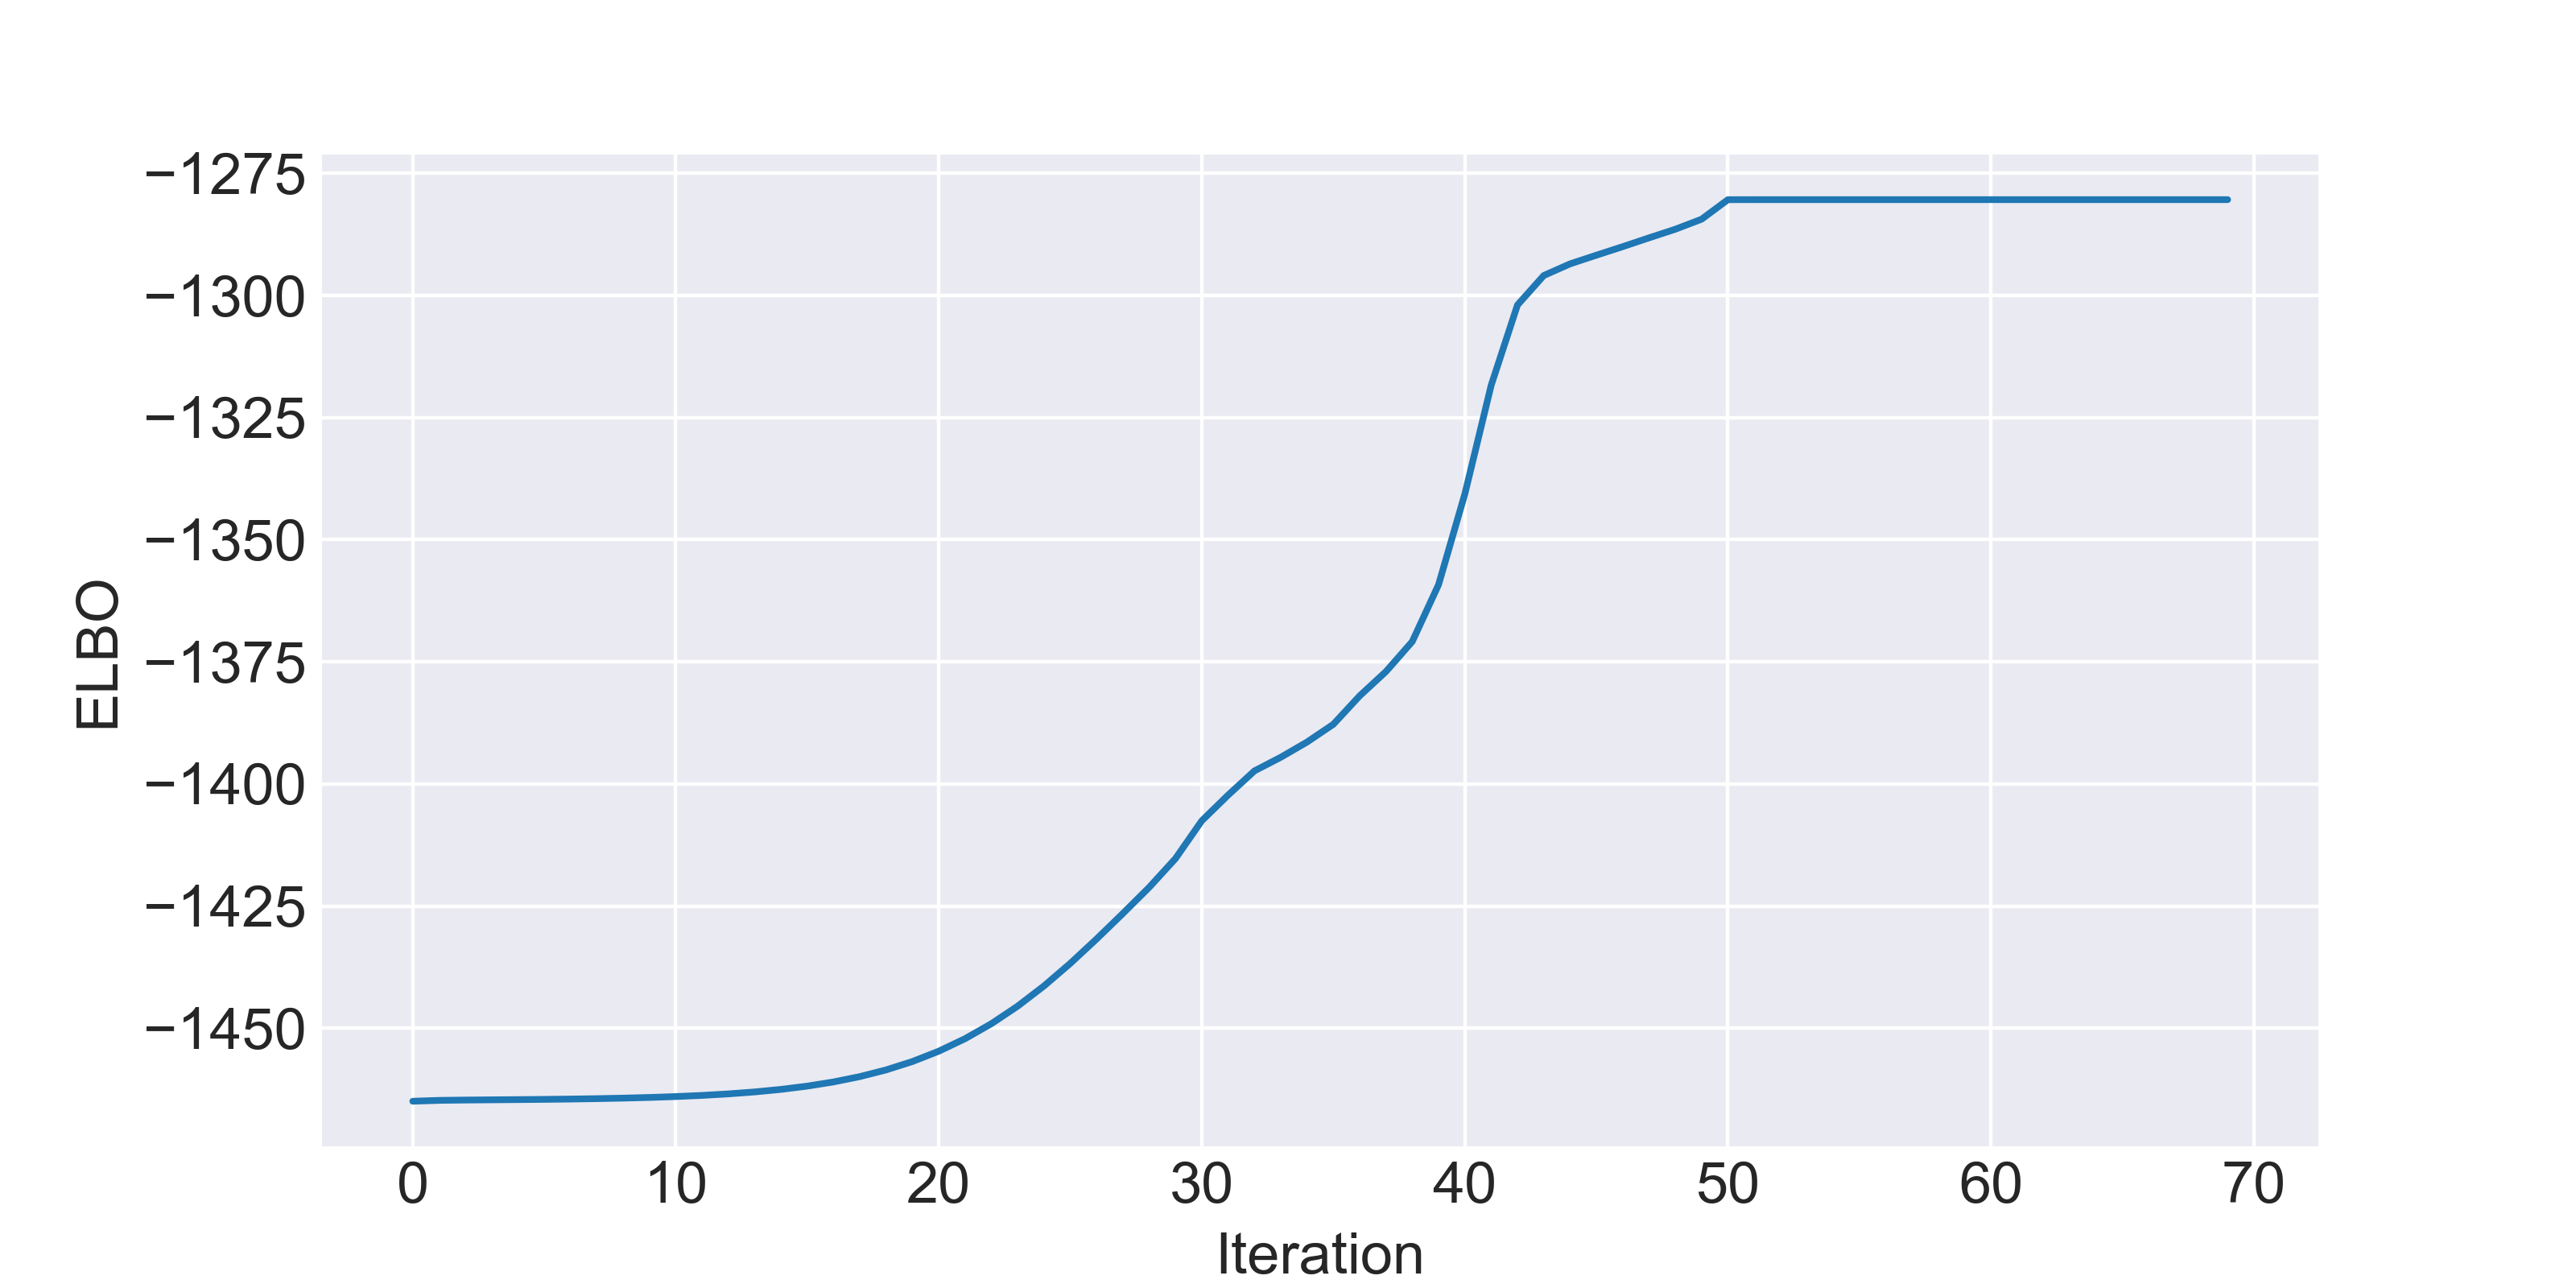
\includegraphics[width=\linewidth]{outputs/old_faithful/elbo.png}
     \caption{ELBO}
  \end{subfigure}
  \begin{subfigure}[b]{0.45\linewidth}
    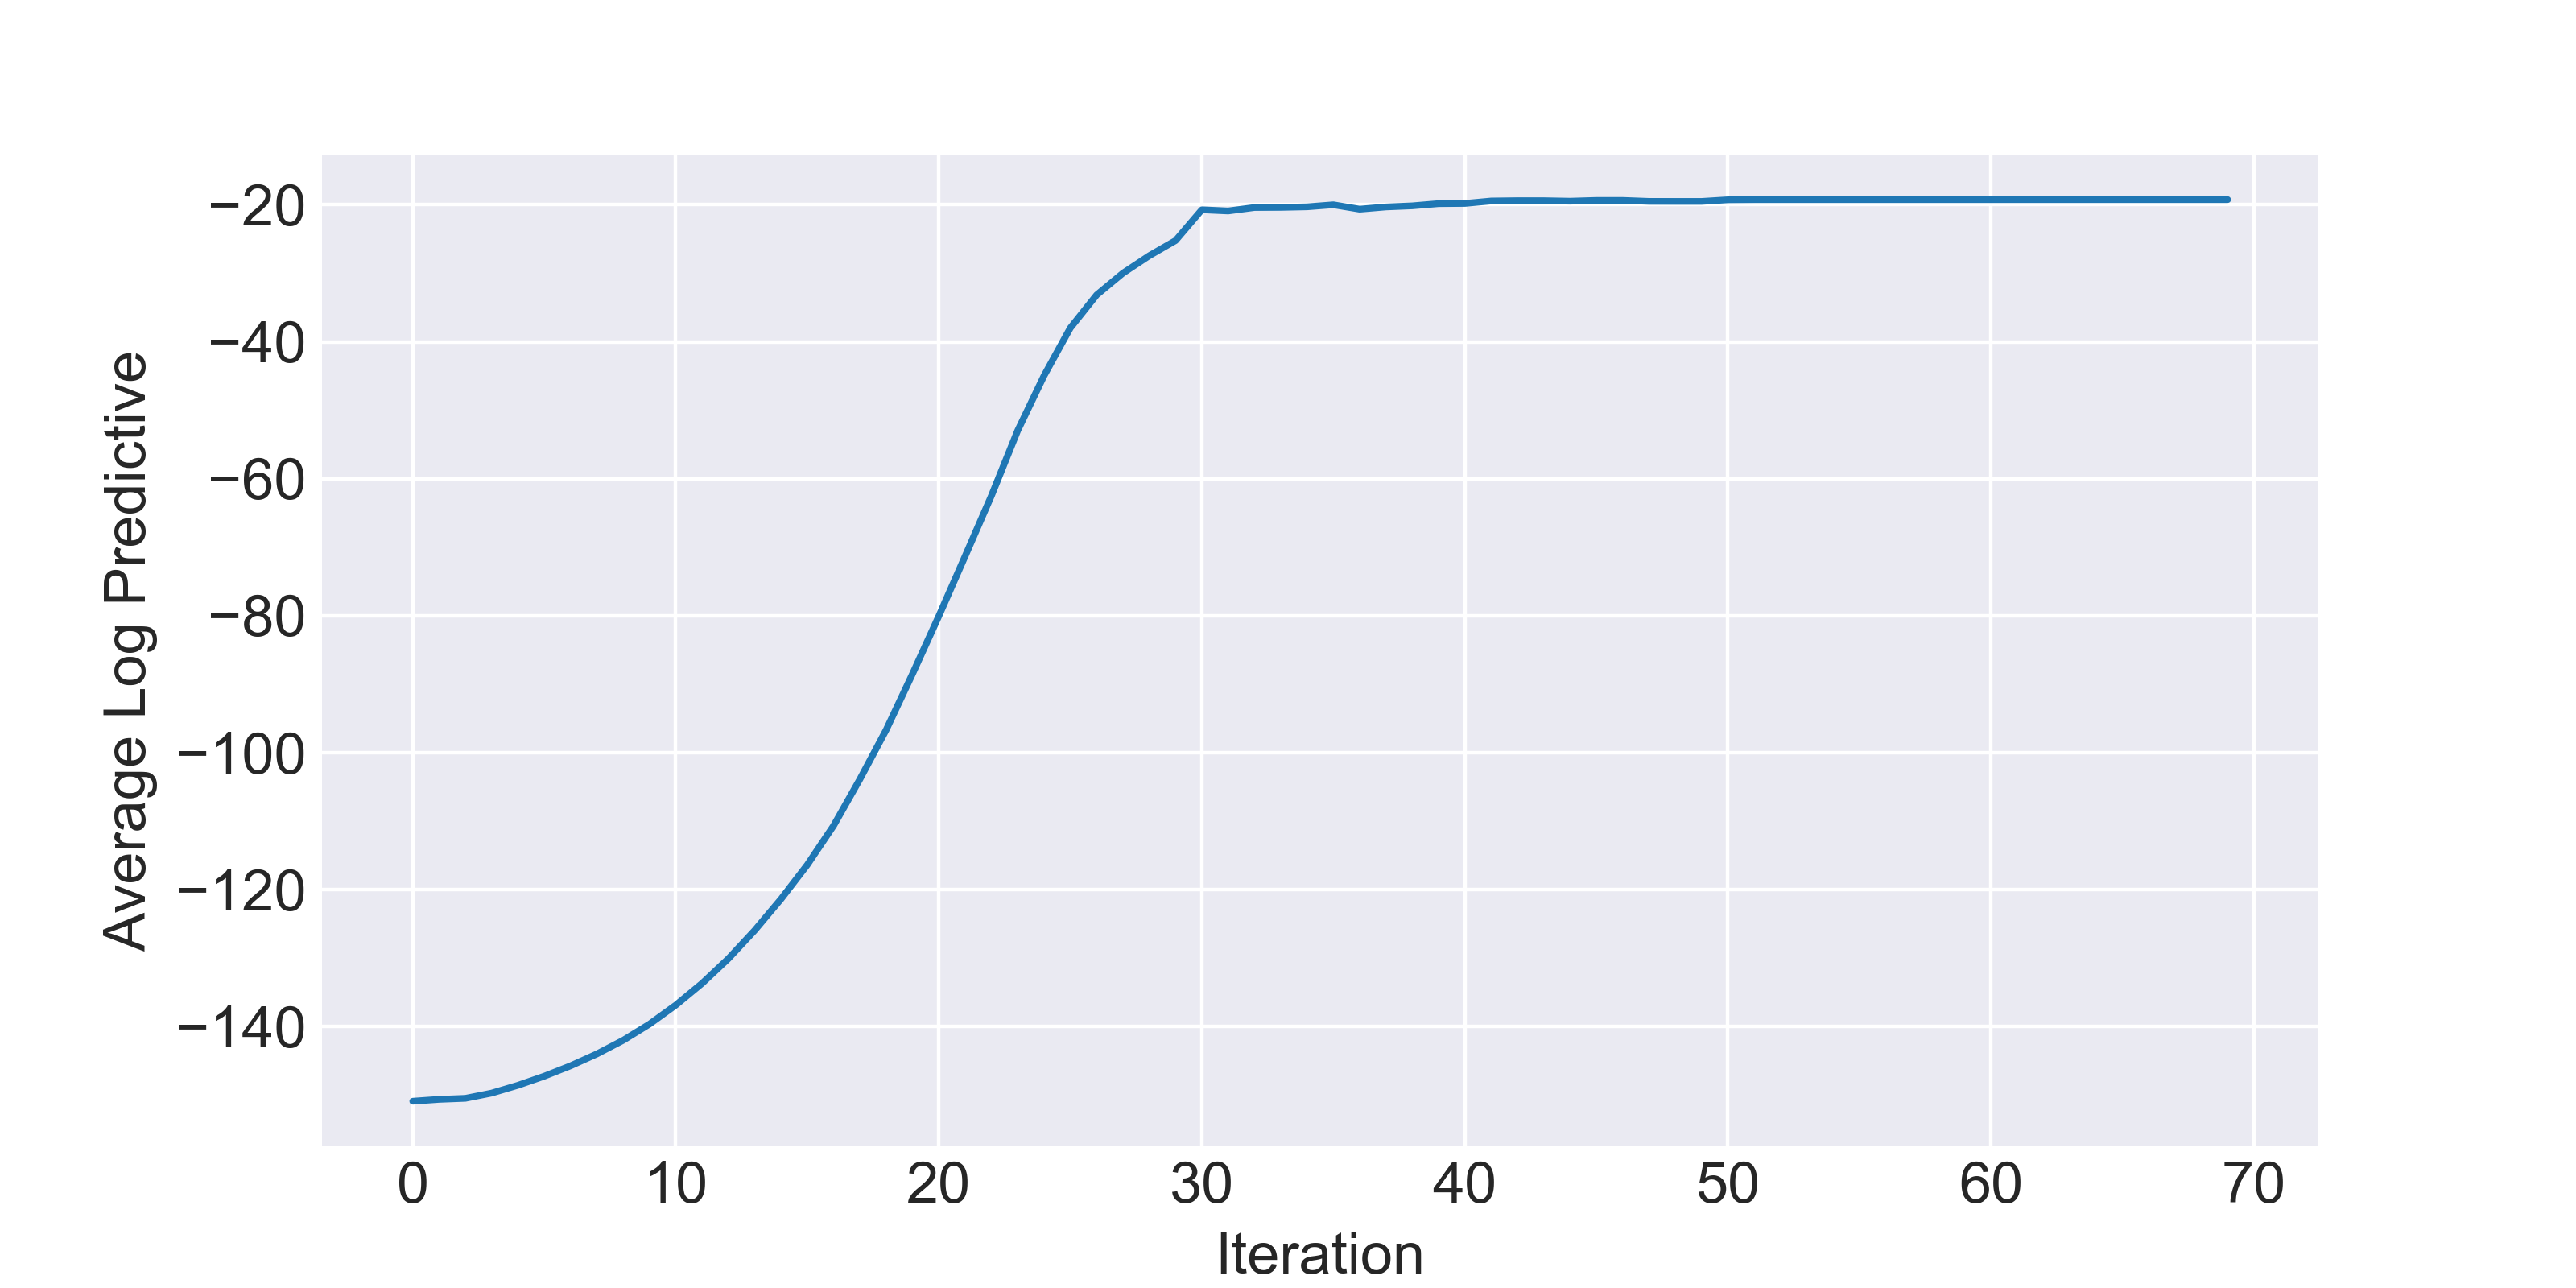
\includegraphics[width=\linewidth]{outputs/old_faithful/pred_density.png}
    \caption{Average Log Predictive}
  \end{subfigure}
  \caption{The figure (a) shows successive improvement on the evidence lower bound while the figure (b) shows the average of the log predictive calculated on the original old faithful dataset, since there is no testing dataset.}
%  \label{fig:coffee3}
\end{figure}

\subsection{Image Grouping}

\subsubsection{Grouping using CAVI}

Consider the task of grouping image according to their color profiles for the imageCLEF dataset \citep{villegas2014overview}. The dataset was initially a database of over 31 million images was created by querying Google, Bing and Yahoo!. Then a subset of 250,000 images was selected from this database by choosing the top images from a ranked list. We randomly select \textbf{5 thousand} images from the imageCLEF collection as our dataset to do the image grouping.

One approach to group image according to their color profiles is to compute the color histogram of the images. Figure \ref{fig:hist1} shows the blue, green and red channel histograms of one images from the imageCLEF data. Each histogram is a vector of length 256, counting the number of pixel in the range of (0 to 255) in each channel. Concatenating the three color histogram gives a 768-dimensional representation of each image, regardless of its original size in pixel-space.

\begin{figure}[H]
  \centering
    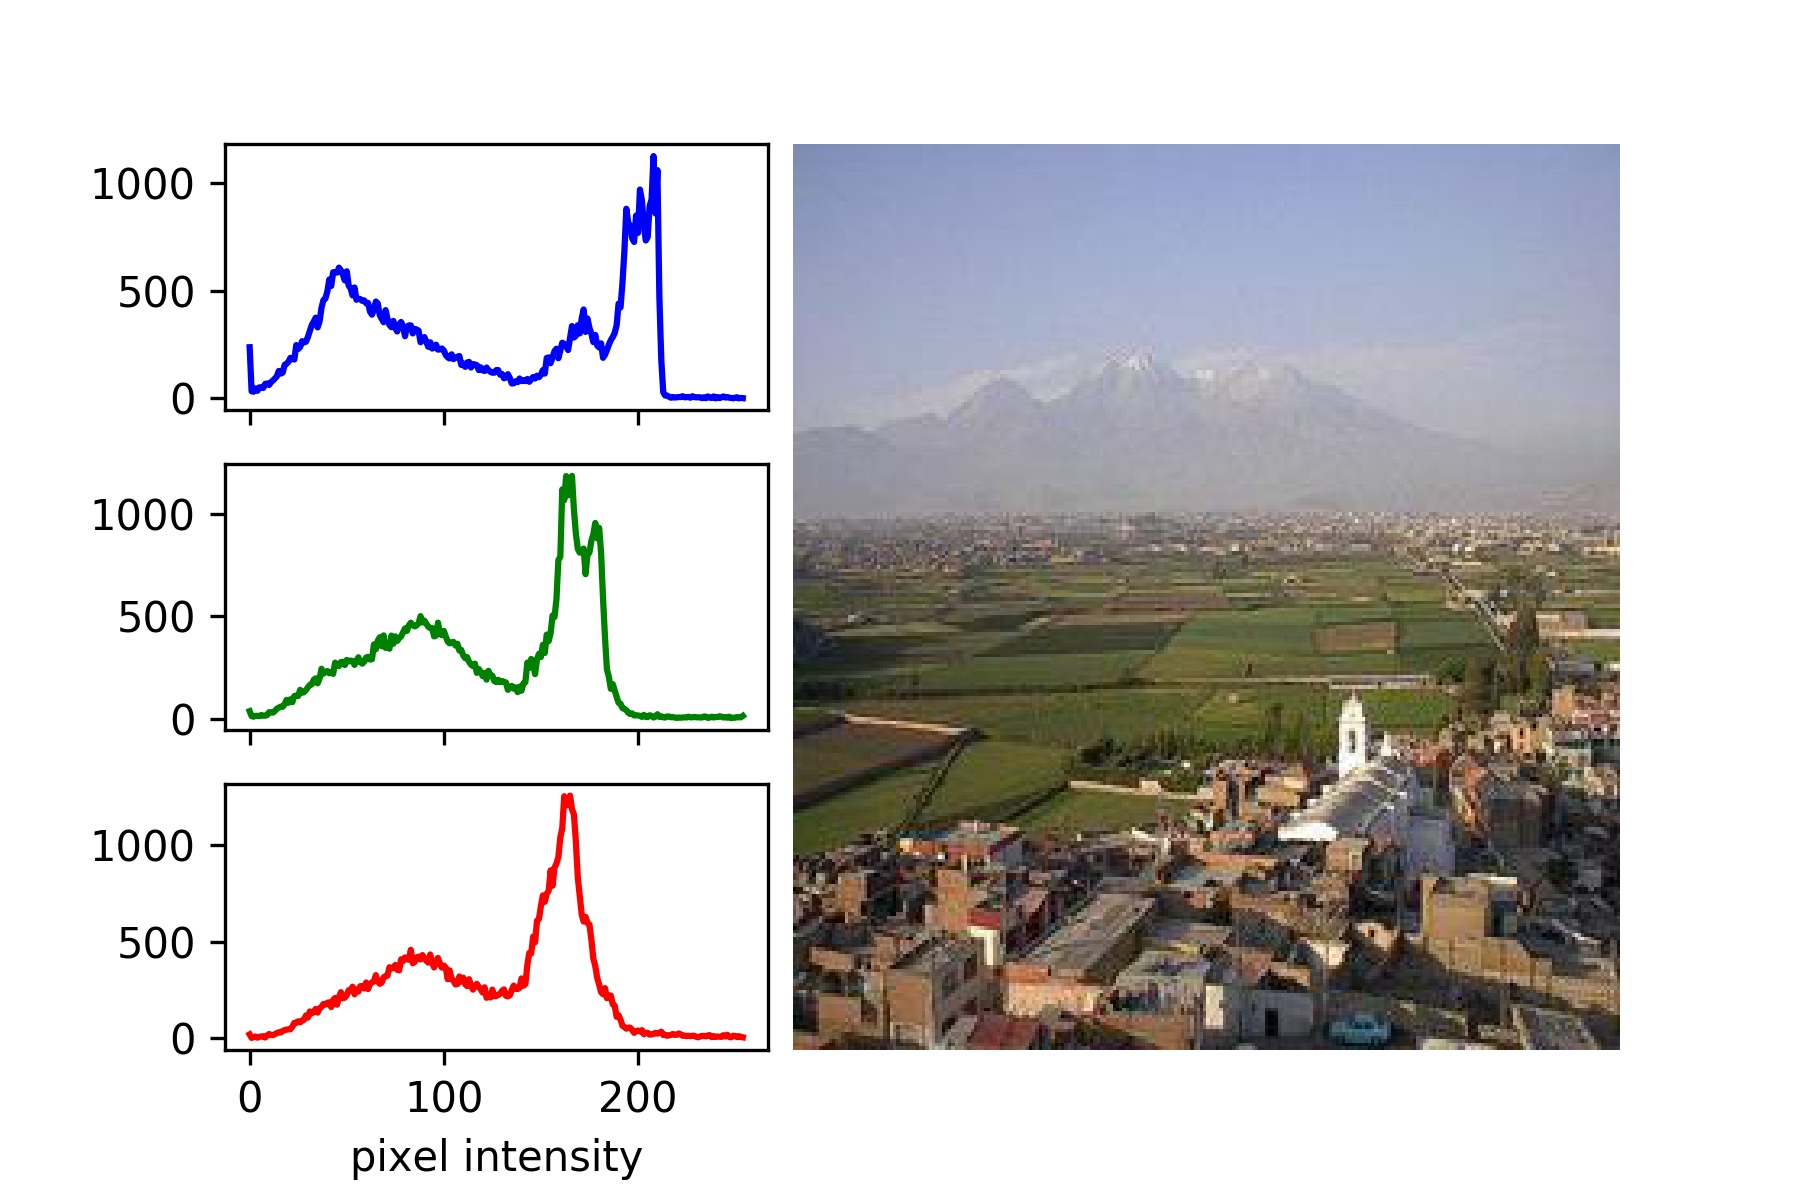
\includegraphics[width=5in, height=2.8in]{outputs/report_figs/hist_demo.jpeg}
  \caption{The left three histograms shows pixel counts on Blue, Green and Red channels for the right picture (from the imageCLEF datasets) respectively. The pixel intensity ranges from 0-255. So we use a 768 dimensional vector to characterize an image.}
\label{fig:hist1}
\end{figure}

We use the CAVI Algorithm \ref{alg:3} to fit a Gaussian mixture models with thirty clusters to the image histograms for the 5000 images. Figure \ref{fig:hist2} shows similarly colored images assigned to three randomly chosen clusters. We could see that the CAVI Algorithm \ref{alg:3} could group the images well according to their color files.

\begin{figure}[H]
  \centering
  \begin{subfigure}[b]{0.36\linewidth}
    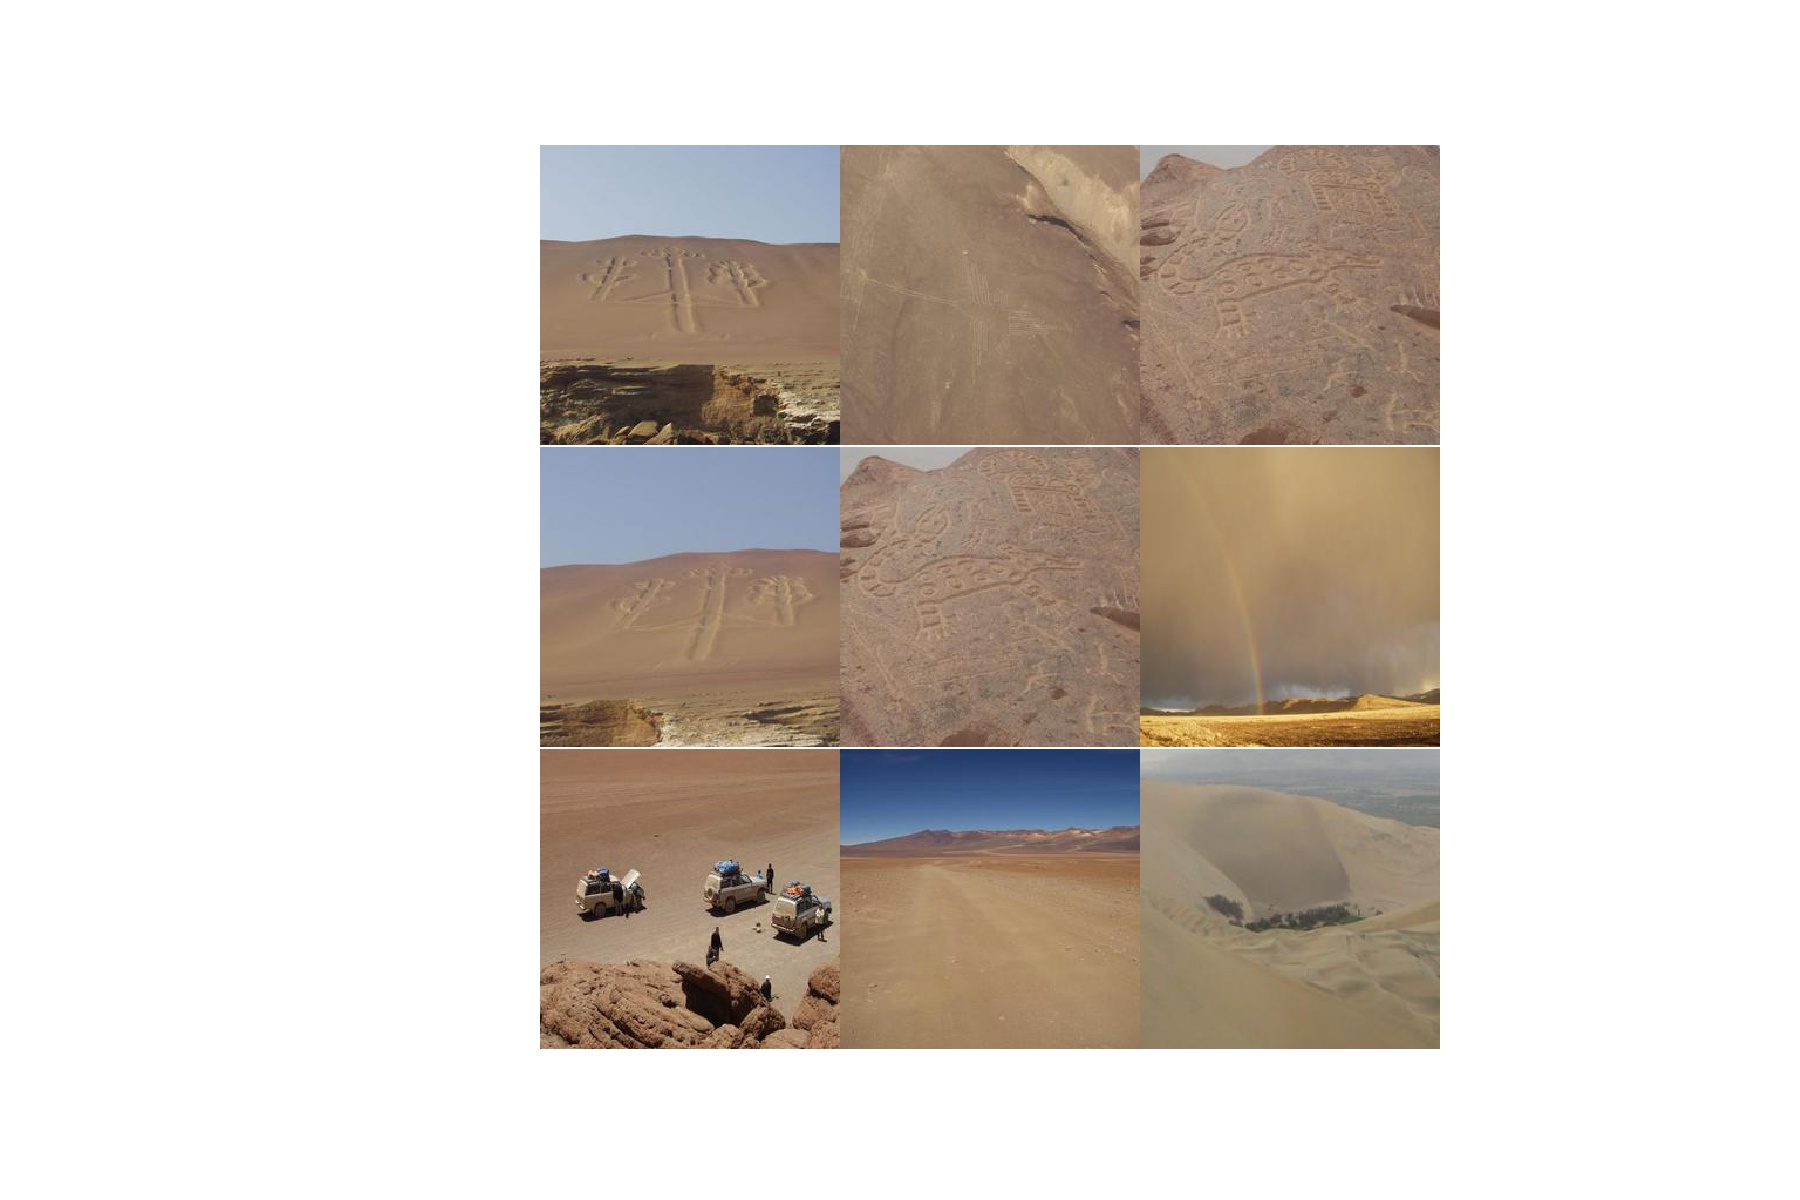
\includegraphics[trim=5.5cm 5.5cm 5.5cm 5.5cm,clip=true,width=\linewidth]{outputs/report_figs/2.jpg}
     \caption{Yellow}
  \end{subfigure}
  \hspace*{-2.8em}
  \begin{subfigure}[b]{0.36\linewidth}
    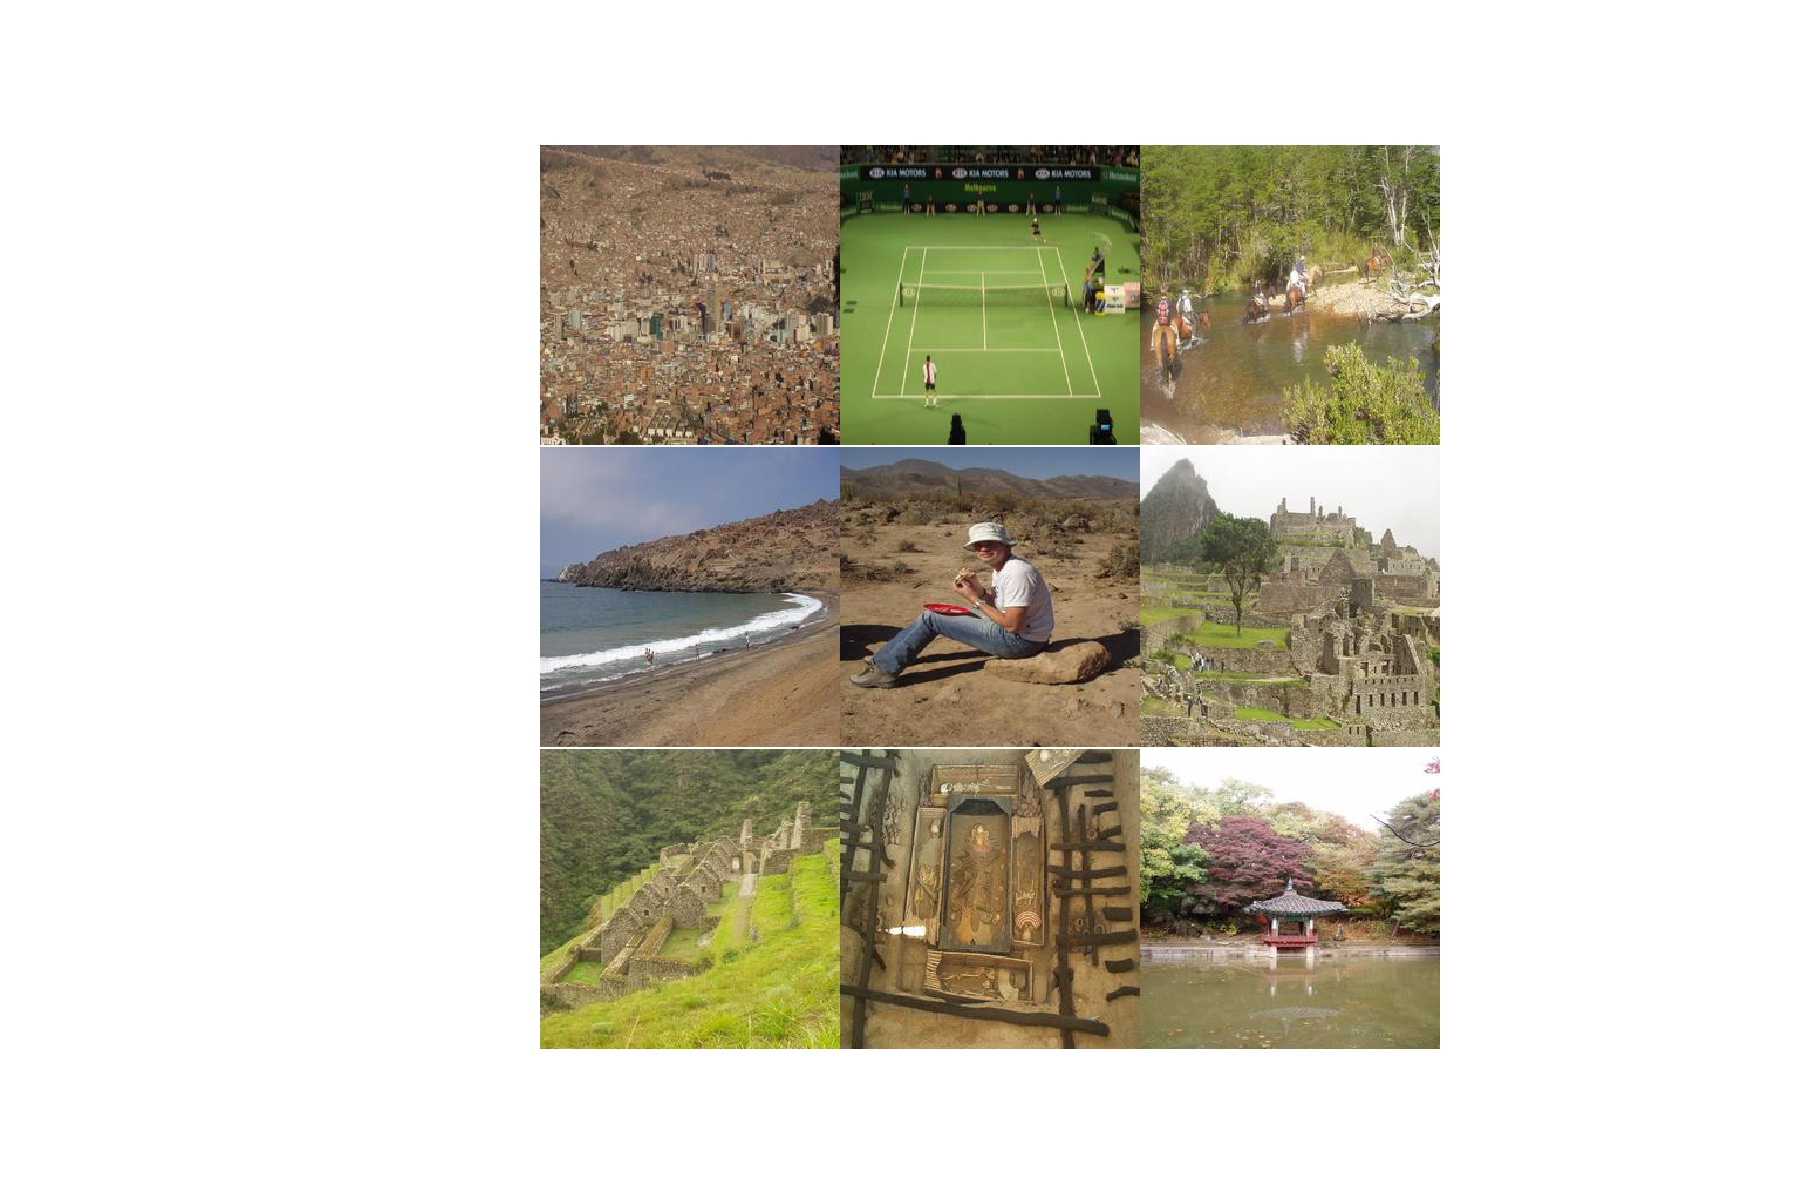
\includegraphics[trim=5.5cm 5.5cm 5.5cm 5.5cm,clip=true,width=\linewidth]{outputs/report_figs/10.jpg}
    \caption{Green}
  \end{subfigure}
  \hspace*{-2.8em}
  \begin{subfigure}[b]{0.36\linewidth}
    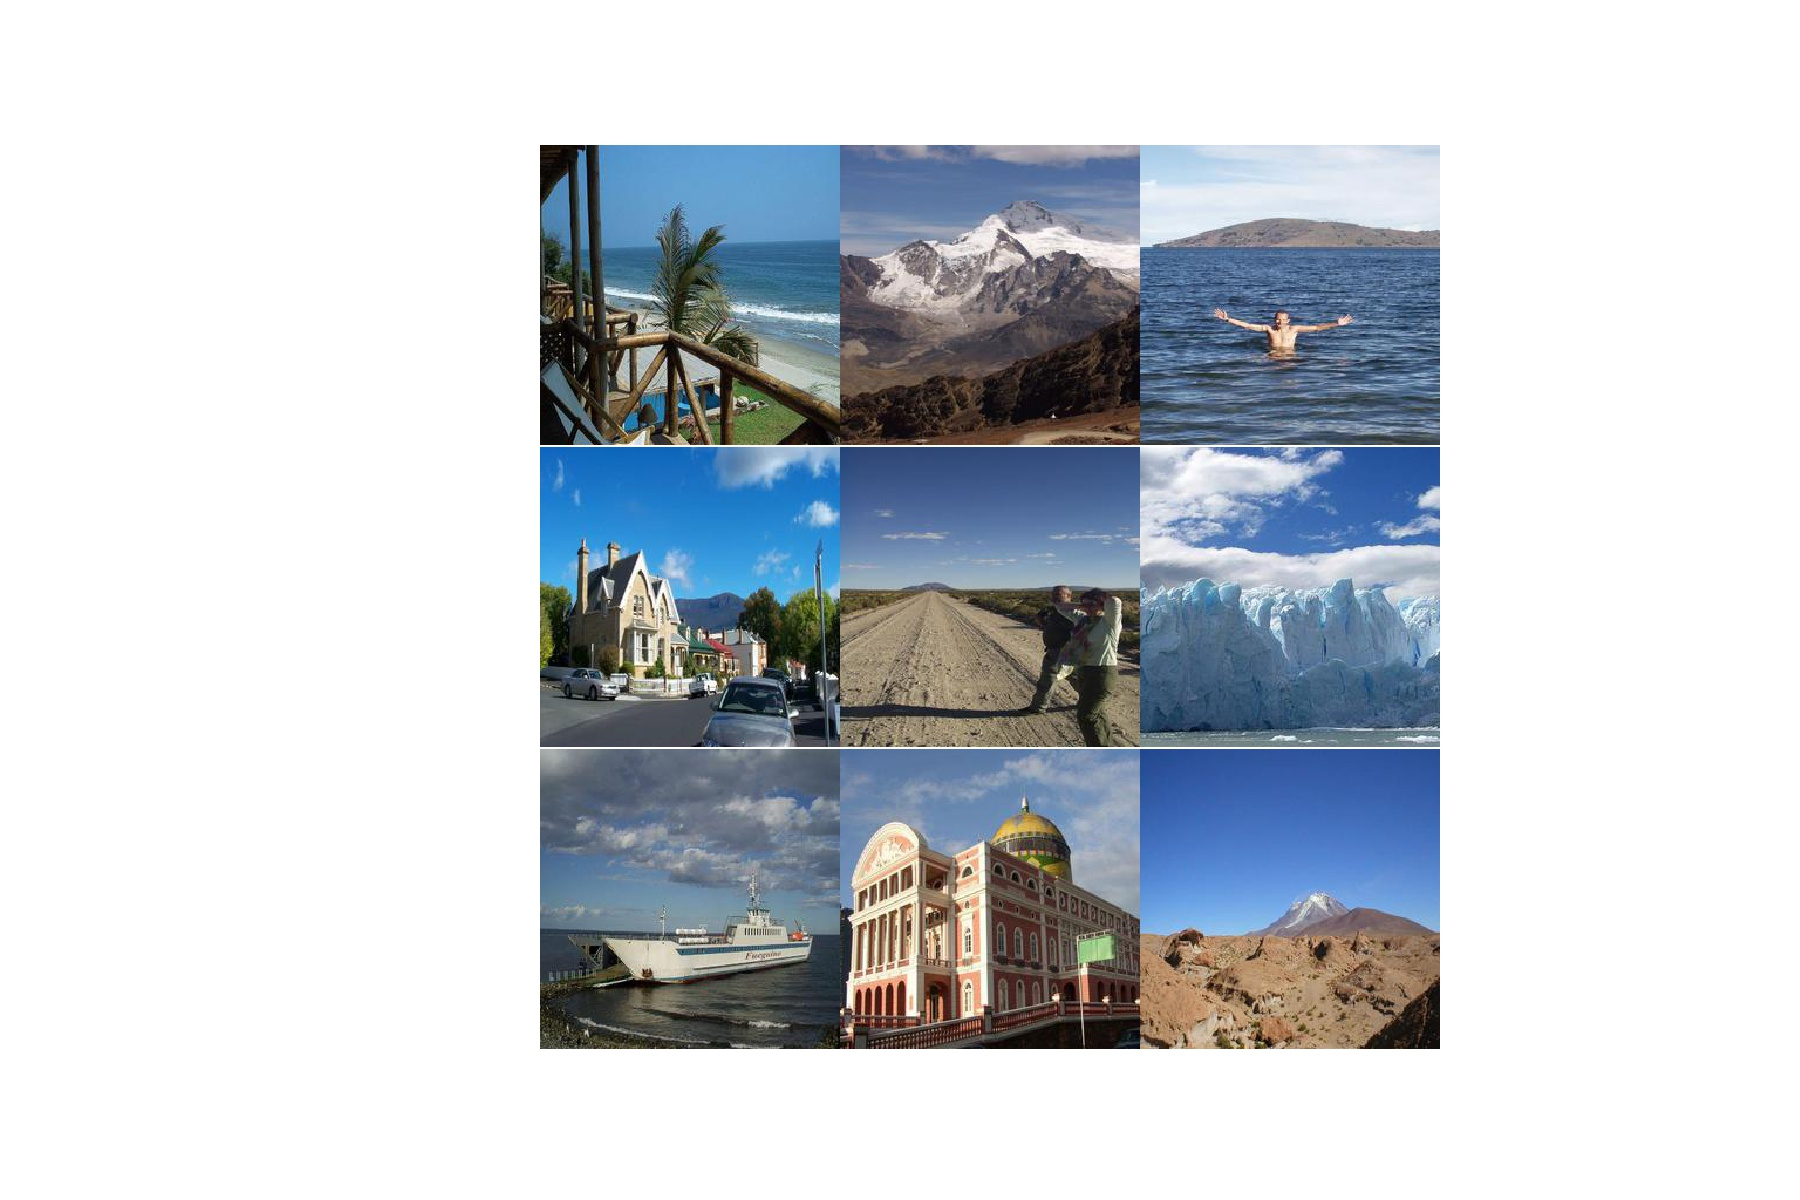
\includegraphics[trim=5.5cm 5.5cm 5.5cm 5.5cm,clip=true,width=\linewidth]{outputs/report_figs/16.jpg}
    \caption{Blue}
  \end{subfigure}
  \caption{Classification results based on the mixture of Gaussians. Three subfigures show nine randomly sampled images from three clusters. We name each cluster by its dominant color.}
\label{fig:hist2}
\end{figure}

\subsubsection{Comparison with MCMC}

For this image histogram clustering problem, we compare the CAVI to an implementation in Stan, the same as in Appendix B in \citep{blei2017variational}, which No-U-Turn sampler(NUTS)\citep{carpenter2017stan} \citep{hoffman2012stan}. Stan is a probabilistic programming language for statistical inference written in C++. Stan implements gradient-based Markov chain Monte Carlo (MCMC) algorithms for Bayesian inference

When using the CAVI to fit a Gaussian mixture models with thirty clusters to the image histograms for the 5000 images, the ELBO converges in less than 1 minute, which means the CAVI could finish the parameter estimation within 1 minute. However, when using the NUTS in Stan, even with a simpler setting, fitting a diagonal covariance Gaussian mixture models with thirty clusters, it takes for more than two hours to run for only 60 iterations, which has been tested to be far from convergence.

Therefore, we could see that variational inference provides a better approach to approximate bayesian inference when dealing with large dataset and complex models.

\section{Discussion and Extension}

The mixture Gaussian model is a special case for conditionally conjugate models with local and global variables. Models like this come up frequently in Bayesian statistics and statistical machine learning, where the global variables are parameters and the local variables are latent variables. A close form of coordinate ascent variational inference(CAVI) algorithm could be derived for this general class of models. 

Modern applications of probability models may analyze massive dataset and the mean-field variational inference could be scaled to big data using stochastic variational inference(SVI) \citep{hoffman2013stochastic}. The CAVI algorithm could not scale to large dataset since it requires iterating through the entire data set at each iteration. As the data size grows, each iteration becomes too computational expensive. Hence instead of using coordinate ascent, a gradient-based optimization which climbs the ELBO by computing and following its gradient at each iteration was proposed. And that's the key idea of stochastic variational inference(SVI). The algorithm of SVI is simple, it repeatedly (a)subsample a data point from the full dataset, (b) use natural gradient-based stochastic optimization method to update the parameters with the subsampled data. This stochastic optimization could give noisy but cheap-to-compute gradients to reach the optimum of the ELBO. In the paper \citep{robbins1951textordfemininea}, they proved results implying this stochastic optimization could successfully use the noisy unbiased gradients under certain condition. And this SVI could enable the modern machine learning to big data \citep{bottou2004large}. 

\bibliographystyle{plainnat}
\bibliography{reference}

\end{document}